\documentclass[11pt,a4paper,twoside]{article}

\usepackage[utf8]{inputenc}
\usepackage[T1]{fontenc}
\usepackage[margin=1in]{geometry}
\usepackage{amsmath,amssymb,amsthm}\usepackage{stmaryrd}
\usepackage{graphicx}
\usepackage{booktabs}
\usepackage{hyperref}
\usepackage{cite}
\usepackage{algorithm}
\usepackage{algpseudocode}
\usepackage{tikz}\usetikzlibrary{positioning}
\usepackage{listings}
\usepackage{xcolor}
\usepackage{cleveref}
\usepackage{url}
\usepackage{multirow}
\usepackage{array}

\theoremstyle{definition}
\newtheorem{definition}{Definition}[section]
\newtheorem{theorem}{Theorem}[section]

% Auto-generated reproducibility macros (regenerated by scripts/generate_tables.py,
% or by scripts/generate_paper.py for the Makefile/CI path)
\IfFileExists{generated/reproducibility.tex}{\input{generated/reproducibility.tex}}{
  \providecommand{\generatedcpu}{(unknown)}
  \providecommand{\generatedmemory}{(unknown)}
  \providecommand{\generatedos}{(unknown)}
  \providecommand{\generatedhash}{(unknown)}
  \providecommand{\generatedpython}{(unknown)}
  \providecommand{\generateduvlock}{(unknown)}
  \providecommand{\generatedchecksum}{(unknown)}
  \providecommand{\generatedseed}{(unknown)}
  \providecommand{\generateddate}{(unknown)}
}

% Auto-generated verification counts (regenerated by scripts/generate_tables.py)
\IfFileExists{tables/verification_counts.tex}{% Auto-generated by scripts/generate_tables.py from
% results/paper_suite_summary.json, results/lubm_benchmark.json, and
% results/wikidata_case_study.json. Do not edit by hand.
\providecommand{\verifiedcount}{45}
\providecommand{\verifiedtotal}{45}
}{
  \providecommand{\verifiedcount}{(unknown)}
  \providecommand{\verifiedtotal}{(unknown)}
}

% Auto-generated headline-range macros (regenerated by scripts/generate_tables.py).
% Speedup macros are baseline/SFDB mean ratios (above 1 = SFDB faster);
% memory macros are SFDB/baseline cost ratios. Prose uses these so the
% abstract's numbers regenerate with the benchmark rather than being
% hand-transcribed.
\IfFileExists{tables/summary_macros.tex}{% Auto-generated by scripts/generate_tables.py from results/paper_suite_summary.json
% Do not edit by hand. Speedup macros are baseline/SFDB mean ratios
% (above 1 = SFDB faster); memory macros are SFDB/baseline cost ratios.
\providecommand{\rangelookupkg}{$18$--$34\times$}
\providecommand{\rangelookupkgmem}{$7.1$--$22\times$}
\providecommand{\rangeglobalkg}{$47$--$79\times$}
\providecommand{\rangeglobalkgmem}{$16$--$37\times$}
\providecommand{\rangecontextkg}{$1.97$--$25\times$}
\providecommand{\rangecontextkgmem}{$1.31$--$12\times$}
\providecommand{\rangetemporalkg}{$1.18$--$1.98\times$}
\providecommand{\rangetemporalkgmem}{$0.52$--$1.27\times$}
\providecommand{\rangetemporalunbkg}{$1.13$--$2.74\times$}
\providecommand{\rangetemporalunbkgmem}{$0.70$--$1.62\times$}
\providecommand{\rangeinsertkg}{$1.06$--$1.28\times$}
\providecommand{\insertkgsmallestscale}{$0.96\times$}
\providecommand{\rangememkg}{$1.78$--$2.47\times$}
\providecommand{\rangememkgmem}{$1.87$--$1.90\times$}
\providecommand{\benchscales}{$100$, $1\,000$, $10\,000$, $100\,000$}
\providecommand{\benchscalecount}{4}
}{
  \providecommand{\rangelookupkg}{(unknown)}
  \providecommand{\rangelookupkgmem}{(unknown)}
  \providecommand{\rangeglobalkg}{(unknown)}
  \providecommand{\rangeglobalkgmem}{(unknown)}
  \providecommand{\rangecontextkg}{(unknown)}
  \providecommand{\rangecontextkgmem}{(unknown)}
  \providecommand{\rangetemporalkg}{(unknown)}
  \providecommand{\rangetemporalkgmem}{(unknown)}
  \providecommand{\rangetemporalunbkg}{(unknown)}
  \providecommand{\rangetemporalunbkgmem}{(unknown)}
  \providecommand{\rangeinsertkg}{(unknown)}
  \providecommand{\rangememkg}{(unknown)}
  \providecommand{\rangememkgmem}{(unknown)}
  \providecommand{\benchscales}{(unknown)}
  \providecommand{\benchscalecount}{(unknown)}
}

% Auto-generated Jena TDB2 comparison macros (regenerated by
% scripts/generate_tables.py from results/jena_reference.json, itself
% produced by scripts/jena_reference.py against a running Fuseki server
% -- see paper/sections/artifact.tex).
\IfFileExists{tables/jena_macros.tex}{% Auto-generated by scripts/generate_tables.py from results/jena_reference.json
% Do not edit by hand. Ratios are jena_mean/sfdb_mean (above 1 = SFDB faster).
% The *large macros are single-scale point estimates at the largest
% scale measured, not ranges -- see the module docstring above.
\providecommand{\jenaavailable}{true}
\providecommand{\jenalargescale}{$100000$}
\providecommand{\rangelookupjena}{$2.44$--$666\times$}
\providecommand{\lookupjenalarge}{$2.44\times$}
\providecommand{\rangeglobaljena}{$8.8$--$432\times$}
\providecommand{\globaljenalarge}{$8.8\times$}
\providecommand{\rangecontextjena}{$2.00$--$237\times$}
\providecommand{\contextjenalarge}{$2.00\times$}
\providecommand{\rangetemporaljena}{$0.15$--$35\times$}
\providecommand{\temporaljenalarge}{$0.15\times$}
\providecommand{\rangetemporalunbjena}{$0.26$--$30\times$}
\providecommand{\temporalunbjenalarge}{$0.26\times$}
}{
  \providecommand{\jenaavailable}{false}
  \providecommand{\jenalargescale}{(unknown)}
  \providecommand{\rangelookupjena}{(unknown)}
  \providecommand{\rangeglobaljena}{(unknown)}
  \providecommand{\rangecontextjena}{(unknown)}
  \providecommand{\rangetemporaljena}{(unknown)}
  \providecommand{\rangetemporalunbjena}{(unknown)}
  \providecommand{\lookupjenalarge}{(unknown)}
  \providecommand{\globaljenalarge}{(unknown)}
  \providecommand{\contextjenalarge}{(unknown)}
  \providecommand{\temporaljenalarge}{(unknown)}
  \providecommand{\temporalunbjenalarge}{(unknown)}
}

% Auto-generated Virtuoso comparison macros (regenerated by
% scripts/generate_tables.py from results/virtuoso_reference.json, itself
% produced by scripts/virtuoso_reference.py against a running Virtuoso
% instance -- see paper/sections/artifact.tex).
\IfFileExists{tables/virtuoso_macros.tex}{% Auto-generated by scripts/generate_tables.py from results/virtuoso_reference.json
% Do not edit by hand. Ratios are virtuoso_mean/sfdb_mean (above 1 = SFDB faster).
% The *large macros are single-scale point estimates at the largest
% scale measured, not ranges -- see the module docstring above.
\providecommand{\virtuosoavailable}{true}
\providecommand{\virtuosolargescale}{$100000$}
\providecommand{\rangelookupvirtuoso}{$3.3$--$536\times$}
\providecommand{\lookupvirtuosolarge}{$3.3\times$}
\providecommand{\rangeglobalvirtuoso}{$15$--$508\times$}
\providecommand{\globalvirtuosolarge}{$15\times$}
\providecommand{\rangecontextvirtuoso}{$3.7$--$201\times$}
\providecommand{\contextvirtuosolarge}{$3.7\times$}
\providecommand{\rangetemporalvirtuoso}{$0.14$--$32\times$}
\providecommand{\temporalvirtuosolarge}{$0.14\times$}
\providecommand{\rangetemporalunbvirtuoso}{$0.25$--$20\times$}
\providecommand{\temporalunbvirtuosolarge}{$0.25\times$}
}{
  \providecommand{\virtuosoavailable}{false}
  \providecommand{\virtuosolargescale}{(unknown)}
  \providecommand{\rangelookupvirtuoso}{(unknown)}
  \providecommand{\rangeglobalvirtuoso}{(unknown)}
  \providecommand{\rangecontextvirtuoso}{(unknown)}
  \providecommand{\rangetemporalvirtuoso}{(unknown)}
  \providecommand{\rangetemporalunbvirtuoso}{(unknown)}
  \providecommand{\lookupvirtuosolarge}{(unknown)}
  \providecommand{\globalvirtuosolarge}{(unknown)}
  \providecommand{\contextvirtuosolarge}{(unknown)}
  \providecommand{\temporalvirtuosolarge}{(unknown)}
  \providecommand{\temporalunbvirtuosolarge}{(unknown)}
}

% Auto-generated GraphDB comparison macros (regenerated by
% scripts/generate_tables.py from results/graphdb_reference.json, itself
% produced by scripts/graphdb_reference.py against a running GraphDB
% instance -- see paper/sections/artifact.tex).
\IfFileExists{tables/graphdb_macros.tex}{% Auto-generated by scripts/generate_tables.py from results/graphdb_reference.json
% Do not edit by hand. Ratios are graphdb_mean/sfdb_mean (above 1 = SFDB faster).
% The *large macros are single-scale point estimates at the largest
% scale measured, not ranges -- see the module docstring above.
\providecommand{\graphdbavailable}{true}
\providecommand{\graphdblargescale}{$100000$}
\providecommand{\rangelookupgraphdb}{$1.80$--$465\times$}
\providecommand{\lookupgraphdblarge}{$1.80\times$}
\providecommand{\rangeglobalgraphdb}{$6.3$--$499\times$}
\providecommand{\globalgraphdblarge}{$6.3\times$}
\providecommand{\rangecontextgraphdb}{$1.63$--$244\times$}
\providecommand{\contextgraphdblarge}{$1.63\times$}
\providecommand{\rangetemporalgraphdb}{$0.16$--$34\times$}
\providecommand{\temporalgraphdblarge}{$0.16\times$}
\providecommand{\rangetemporalunbgraphdb}{$0.22$--$29\times$}
\providecommand{\temporalunbgraphdblarge}{$0.22\times$}
}{
  \providecommand{\graphdbavailable}{false}
  \providecommand{\graphdblargescale}{(unknown)}
  \providecommand{\rangelookupgraphdb}{(unknown)}
  \providecommand{\rangeglobalgraphdb}{(unknown)}
  \providecommand{\rangecontextgraphdb}{(unknown)}
  \providecommand{\rangetemporalgraphdb}{(unknown)}
  \providecommand{\rangetemporalunbgraphdb}{(unknown)}
  \providecommand{\lookupgraphdblarge}{(unknown)}
  \providecommand{\globalgraphdblarge}{(unknown)}
  \providecommand{\contextgraphdblarge}{(unknown)}
  \providecommand{\temporalgraphdblarge}{(unknown)}
  \providecommand{\temporalunbgraphdblarge}{(unknown)}
}

% Auto-generated LUBM standard-benchmark-workload macros (regenerated by
% scripts/generate_tables.py from results/lubm_benchmark.json, itself
% produced by scripts/lubm_benchmark.py -- see paper/sections/evaluation.tex).
\IfFileExists{tables/lubm_macros.tex}{% Auto-generated by scripts/generate_tables.py from results/lubm_benchmark.json
% Do not edit by hand. Ratios are engine_mean/sfdb_mean (above 1 = SFDB faster).
\providecommand{\lubmavailable}{true}
\providecommand{\lubmlargescale}{$97,289$}
\providecommand{\lubmnumfacts}{$97,289$}
\providecommand{\rangelookuplubmkg}{$5.9$--$11\times$}
\providecommand{\rangelookuplubmkgmem}{$2.71$--$4.3\times$}
\providecommand{\lookuplubmkglarge}{$5.9\times$}
\providecommand{\lookuplubmkgmemlarge}{$2.71\times$}
\providecommand{\rangeloballubmkg}{$42$--$69\times$}
\providecommand{\rangeglobalubmkgmem}{$13$--$28\times$}
\providecommand{\globallubmkglarge}{$45\times$}
\providecommand{\globallubmkgmemlarge}{$23\times$}
\providecommand{\rangecontextlubmkg}{$9.5$--$332\times$}
\providecommand{\rangecontextlubmkgmem}{$2.74$--$3.6\times$}
\providecommand{\contextlubmkglarge}{$332\times$}
\providecommand{\contextlubmkgmemlarge}{$3.6\times$}
\providecommand{\rangetemporallubmkg}{$0.46$--$1.20\times$}
\providecommand{\rangetemporallubmkgmem}{$0.12$--$0.98\times$}
\providecommand{\temporallubmkglarge}{$1.20\times$}
\providecommand{\temporallubmkgmemlarge}{$0.98\times$}
\providecommand{\rangetemporalunblubmkg}{$0.51$--$1.24\times$}
\providecommand{\rangetemporalunblubmkgmem}{$0.17$--$0.94\times$}
\providecommand{\temporalunblubmkglarge}{$1.20\times$}
\providecommand{\temporalunblubmkgmemlarge}{$0.94\times$}
}{
  \providecommand{\lubmavailable}{false}
  \providecommand{\lubmlargescale}{(unknown)}
  \providecommand{\lubmnumfacts}{(unknown)}
  \providecommand{\rangelookuplubmkg}{(unknown)}
  \providecommand{\rangelookuplubmkgmem}{(unknown)}
  \providecommand{\lookuplubmkglarge}{(unknown)}
  \providecommand{\lookuplubmkgmemlarge}{(unknown)}
  \providecommand{\rangeloballubmkg}{(unknown)}
  \providecommand{\rangeglobalubmkgmem}{(unknown)}
  \providecommand{\globallubmkglarge}{(unknown)}
  \providecommand{\globallubmkgmemlarge}{(unknown)}
  \providecommand{\rangecontextlubmkg}{(unknown)}
  \providecommand{\rangecontextlubmkgmem}{(unknown)}
  \providecommand{\contextlubmkglarge}{(unknown)}
  \providecommand{\contextlubmkgmemlarge}{(unknown)}
  \providecommand{\rangetemporallubmkg}{(unknown)}
  \providecommand{\rangetemporallubmkgmem}{(unknown)}
  \providecommand{\temporallubmkglarge}{(unknown)}
  \providecommand{\temporallubmkgmemlarge}{(unknown)}
  \providecommand{\rangetemporalunblubmkg}{(unknown)}
  \providecommand{\rangetemporalunblubmkgmem}{(unknown)}
  \providecommand{\temporalunblubmkglarge}{(unknown)}
  \providecommand{\temporalunblubmkgmemlarge}{(unknown)}
}

% Auto-generated LUBM-vs-external-store macros (regenerated by
% scripts/generate_tables.py from results/lubm_{jena,virtuoso,graphdb}_reference.json,
% themselves produced by scripts/lubm_external_reference.py against a
% running Jena/Virtuoso/GraphDB instance -- see
% paper/sections/evaluation.tex, Section~\ref{sec:eval:lubm}). These vary
% both the dataset (LUBM) and the comparison engine (a real external
% store) simultaneously.
\IfFileExists{tables/lubm_jena_macros.tex}{% Auto-generated by scripts/generate_tables.py from results/lubm_jena_reference.json
% Do not edit by hand. Ratios are external_mean/sfdb_mean (above 1 = SFDB faster).
\providecommand{\lubmjenaavailable}{true}
\providecommand{\lubmjenalargescale}{$97289$}
\providecommand{\rangelookuplubmjena}{$1136$--$3004\times$}
\providecommand{\lookuplubmjenalarge}{$2574\times$}
\providecommand{\rangegloballubmjena}{$8.6$--$368\times$}
\providecommand{\globallubmjenalarge}{$8.6\times$}
\providecommand{\rangecontextlubmjena}{$42$--$136\times$}
\providecommand{\contextlubmjenalarge}{$136\times$}
\providecommand{\rangetemporallubmjena}{$0.10$--$22\times$}
\providecommand{\temporallubmjenalarge}{$0.10\times$}
\providecommand{\rangetemporalunblubmjena}{$0.14$--$26\times$}
\providecommand{\temporalunblubmjenalarge}{$0.14\times$}
}{
  \providecommand{\lubmjenaavailable}{false}
  \providecommand{\lubmjenalargescale}{(unknown)}
  \providecommand{\rangelookuplubmjena}{(unknown)}
  \providecommand{\lookuplubmjenalarge}{(unknown)}
  \providecommand{\rangegloballubmjena}{(unknown)}
  \providecommand{\globallubmjenalarge}{(unknown)}
  \providecommand{\rangecontextlubmjena}{(unknown)}
  \providecommand{\contextlubmjenalarge}{(unknown)}
  \providecommand{\rangetemporallubmjena}{(unknown)}
  \providecommand{\temporallubmjenalarge}{(unknown)}
  \providecommand{\rangetemporalunblubmjena}{(unknown)}
  \providecommand{\temporalunblubmjenalarge}{(unknown)}
}
\IfFileExists{tables/lubm_virtuoso_macros.tex}{% Auto-generated by scripts/generate_tables.py from results/lubm_virtuoso_reference.json
% Do not edit by hand. Ratios are external_mean/sfdb_mean (above 1 = SFDB faster).
\providecommand{\lubmvirtuosoavailable}{true}
\providecommand{\lubmvirtuosolargescale}{$97289$}
\providecommand{\rangelookuplubmvirtuoso}{$682$--$1960\times$}
\providecommand{\lookuplubmvirtuosolarge}{$1801\times$}
\providecommand{\rangegloballubmvirtuoso}{$13$--$295\times$}
\providecommand{\globallubmvirtuosolarge}{$13\times$}
\providecommand{\rangecontextlubmvirtuoso}{$35$--$262\times$}
\providecommand{\contextlubmvirtuosolarge}{$262\times$}
\providecommand{\rangetemporallubmvirtuoso}{$0.10$--$22\times$}
\providecommand{\temporallubmvirtuosolarge}{$0.10\times$}
\providecommand{\rangetemporalunblubmvirtuoso}{$0.11$--$27\times$}
\providecommand{\temporalunblubmvirtuosolarge}{$0.11\times$}
}{
  \providecommand{\lubmvirtuosoavailable}{false}
  \providecommand{\lubmvirtuosolargescale}{(unknown)}
  \providecommand{\rangelookuplubmvirtuoso}{(unknown)}
  \providecommand{\lookuplubmvirtuosolarge}{(unknown)}
  \providecommand{\rangegloballubmvirtuoso}{(unknown)}
  \providecommand{\globallubmvirtuosolarge}{(unknown)}
  \providecommand{\rangecontextlubmvirtuoso}{(unknown)}
  \providecommand{\contextlubmvirtuosolarge}{(unknown)}
  \providecommand{\rangetemporallubmvirtuoso}{(unknown)}
  \providecommand{\temporallubmvirtuosolarge}{(unknown)}
  \providecommand{\rangetemporalunblubmvirtuoso}{(unknown)}
  \providecommand{\temporalunblubmvirtuosolarge}{(unknown)}
}
\IfFileExists{tables/lubm_graphdb_macros.tex}{% Auto-generated by scripts/generate_tables.py from results/lubm_graphdb_reference.json
% Do not edit by hand. Ratios are external_mean/sfdb_mean (above 1 = SFDB faster).
\providecommand{\lubmgraphdbavailable}{true}
\providecommand{\lubmgraphdblargescale}{$97289$}
\providecommand{\rangelookuplubmgraphdb}{$1157$--$2783\times$}
\providecommand{\lookuplubmgraphdblarge}{$1644\times$}
\providecommand{\rangegloballubmgraphdb}{$5.2$--$201\times$}
\providecommand{\globallubmgraphdblarge}{$5.2\times$}
\providecommand{\rangecontextlubmgraphdb}{$99$--$126\times$}
\providecommand{\contextlubmgraphdblarge}{$126\times$}
\providecommand{\rangetemporallubmgraphdb}{$0.10$--$24\times$}
\providecommand{\temporallubmgraphdblarge}{$0.10\times$}
\providecommand{\rangetemporalunblubmgraphdb}{$0.10$--$24\times$}
\providecommand{\temporalunblubmgraphdblarge}{$0.10\times$}
}{
  \providecommand{\lubmgraphdbavailable}{false}
  \providecommand{\lubmgraphdblargescale}{(unknown)}
  \providecommand{\rangelookuplubmgraphdb}{(unknown)}
  \providecommand{\lookuplubmgraphdblarge}{(unknown)}
  \providecommand{\rangegloballubmgraphdb}{(unknown)}
  \providecommand{\globallubmgraphdblarge}{(unknown)}
  \providecommand{\rangecontextlubmgraphdb}{(unknown)}
  \providecommand{\contextlubmgraphdblarge}{(unknown)}
  \providecommand{\rangetemporallubmgraphdb}{(unknown)}
  \providecommand{\temporallubmgraphdblarge}{(unknown)}
  \providecommand{\rangetemporalunblubmgraphdb}{(unknown)}
  \providecommand{\temporalunblubmgraphdblarge}{(unknown)}
}

% Auto-generated real-world case-study macros (regenerated by
% scripts/generate_tables.py from results/wikidata_case_study.json,
% itself produced by scripts/wikidata_case_study_benchmark.py against a
% cached Wikidata snapshot -- see paper/sections/evaluation.tex).
\IfFileExists{tables/wikidata_case_study_macros.tex}{% Auto-generated by scripts/generate_tables.py from results/wikidata_case_study.json
% Do not edit by hand.
\providecommand{\wikidatacasestudyavailable}{true}
\providecommand{\wikidatanumfacts}{$5,337$}
\providecommand{\wikidatalookupkg}{$0.07\times$}
\providecommand{\wikidatalookupkgmem}{$0.19\times$}
\providecommand{\wikidataglobalkg}{$0.01\times$}
\providecommand{\wikidataglobalkgmem}{$0.03\times$}
\providecommand{\wikidatacontextkg}{$0.02\times$}
\providecommand{\wikidatacontextkgmem}{$0.03\times$}
\providecommand{\wikidatatemporalkg}{$0.37\times$}
\providecommand{\wikidatatemporalkgmem}{$0.85\times$}
\providecommand{\wikidatatemporalunbkg}{$0.33\times$}
\providecommand{\wikidatatemporalunbkgmem}{$0.79\times$}
}{
  \providecommand{\wikidatacasestudyavailable}{false}
  \providecommand{\wikidatanumfacts}{(unknown)}
  \providecommand{\wikidatalookupkg}{(unknown)}
  \providecommand{\wikidatalookupkgmem}{(unknown)}
  \providecommand{\wikidataglobalkg}{(unknown)}
  \providecommand{\wikidataglobalkgmem}{(unknown)}
  \providecommand{\wikidatacontextkg}{(unknown)}
  \providecommand{\wikidatacontextkgmem}{(unknown)}
  \providecommand{\wikidatatemporalkg}{(unknown)}
  \providecommand{\wikidatatemporalkgmem}{(unknown)}
  \providecommand{\wikidatatemporalunbkg}{(unknown)}
  \providecommand{\wikidatatemporalunbkgmem}{(unknown)}
}

\newcommand{\showcpu}{\texttt{\generatedcpu}}
\newcommand{\showmemory}{\texttt{\generatedmemory}}
\newcommand{\showos}{\texttt{\generatedos}}
\newcommand{\githash}{\texttt{\generatedhash}}
\newcommand{\pythonversion}{\texttt{\generatedpython}}
\newcommand{\uvlockhash}{\texttt{\generateduvlock}}
\newcommand{\datachecksum}{\texttt{\generatedchecksum}}
\newcommand{\sfdbseed}{\texttt{\generatedseed}}
\newcommand{\generationdate}{\texttt{\generateddate}}

\title{SFDB: A Context-Indexed Semantic Fact Database with Stalk Indexing\\
       and Verified Cross-Engine Equivalence}

\author{BlackSamuron0305}
\date{}

\begin{document}

\maketitle

\begin{abstract}
Representing semantic knowledge as subject--predicate--object triples forces
higher-arity and context-scoped facts through reification: one statement
becomes many records, and answering a simple lookup becomes a multi-way
join. We describe SFDB, a prototype database whose organising principle is
instead the \emph{context poset}: each fact is stored atomically as a
section over a finite poset of contexts, and entity- and context-anchored
queries are
answered through precomputed indexes rather than reconstruction. The formal
vocabulary is that
of presheaves on a finite Alexandrov space; the sheaf condition holds
vacuously there, and we claim no category-theoretic novelty. A reified
triple-store baseline is co-implemented over the same canonical schema, and
every benchmark query is checked, online, for canonical result equivalence
across engines --- a harness that caught a real semantic bug in our own
engine before publication.

Across \benchscalecount{} scales (\benchscales{} facts), SFDB answers
LOOKUP queries \rangelookupkg{} faster, full-scan GLOBAL queries
\rangeglobalkg{} faster, and CONTEXT queries --- retrieval scoped to a
context and its descendants, the query shape the design is named for ---
\rangecontextkg{} faster than the baseline. A storage-layer control --- the
same baseline with its SQLite tables replaced by in-process dict indexes
--- shows that most of the LOOKUP, GLOBAL, and CONTEXT advantage
(\rangelookupkgmem{}, \rangeglobalkgmem{}, and \rangecontextkgmem{})
survives with the storage-layer difference removed
and is therefore attributable to the design itself. The
temporal-range advantages do not survive the control at all --- SFDB is at
parity or measurably slower than the control on bounded temporal ranges at
most scales --- and insert throughput is slower than the baseline at the
smallest scale measured and faster at every larger one; both are reported
as negative or mixed results rather than smoothed into a single headline.
The cost that funds the advantages that do hold is
memory: \rangememkg{} more resident memory per fact than the baseline.
Against three real, disk-backed production stores accessed over
SPARQL/HTTP --- Apache Jena TDB2, OpenLink Virtuoso, and Ontotext
GraphDB, independently
engineered by three different organisations --- the pattern holds up on LOOKUP,
GLOBAL, and CONTEXT --- SFDB remains faster than all three at every scale, despite
their latencies including an HTTP round trip SFDB's in-process calls do
not pay --- but reverses on TEMPORAL from $10\,000$ facts
onward against all three stores, where a mature production optimiser
overtakes SFDB's Python-level candidate filtering. We report this
crossover as measured rather than smoothing it into either a clean win
or a hedge; that it appears independently against three unrelated
optimisers is evidence it is a property of mature query engines
generally rather than one vendor's implementation. Two further
comparisons --- \wikidatanumfacts{} genuine Wikidata facts we did not
construct, and LUBM, the standard RDF benchmark workload, at four scales
up to \lubmlargescale{} facts --- extend the finding rather than merely
repeat it: LOOKUP, GLOBAL, and CONTEXT reproduce cleanly on both, while
TEMPORAL lands in a different place on each (beating both in-house
baselines on Wikidata, roughly at parity with them on LUBM), direct
evidence that only TEMPORAL among the four query classes is genuinely
sensitive to a dataset's actual shape. Building the LUBM comparison
surfaced the evaluation's most consequential self-correction: a
performance bug in SFDB's own CONTEXT query resolution, present for the
entire evaluation and exposed only by a topology shape (many large,
mutually unrelated top-level contexts) none of this paper's other
datasets have, which required re-running and re-verifying every
CONTEXT number this paper reports and retracting two earlier claims
built on the unfixed numbers. Four external reference points (rdflib, Jena TDB2, Virtuoso, and
GraphDB,
all five query classes, result counts verified against all four), two
real-world/standard-workload comparisons, and ten documented
rounds of self-correction --- including the CONTEXT bug above and a
cross-engine SPARQL semantics divergence found while building the
Virtuoso comparison ---
complete an evaluation built to be checked rather than believed. All
results regenerate from the released artifact with a single command.

\end{abstract}

\section{Introduction}
\label{sec:introduction}

Knowledge graphs have become the default representation for semantic
information on the web and in enterprise systems. Their foundations are simple:
every fact is a triple $(s, p, o)$ that asserts a binary relationship
between a subject, a predicate, and an object~\cite{manola2004rdf,sparql2013}. The
model is uniform, transparent, and has an enormous accumulated tooling base. It
is also a poor fit for large classes of real data.

Two mismatches recur across domains. First, many facts are not binary. A drug
interaction record carries a drug, a target, a dosage, a route, a study population,
and a confidence interval, all in one statement. A financial transaction pairs
a buyer, a seller, an instrument, a price, a currency, a venue, and a
timestamp. Encoding such facts as triples requires \emph{reification}: an
auxiliary event node is minted, each attribute becomes its own triple pointing
at that node, and reconstructing the original fact costs one join per attribute.
Second, the same fact often holds in some contexts and not in others. A
biological interaction that is valid \emph{in vitro} may fail \emph{in vivo};
a corporate policy that applies in the European subsidiary may not apply in
North America. Context is not first-class in the triple model. It is added
either through separate named graphs~\cite{carroll2005named}, through further
reification, or through ad-hoc conventions in the predicate URI.

Both problems have well-known workarounds, and mature triple stores handle
them competently at scale. The question we pose in this paper is whether there
is anything to gain from a database whose primary organising principle is not
the triple but the \emph{context}. Concretely, we ask whether one can build a
storage engine that (i)~stores each fact as an atomic record, without
reification, and (ii)~indexes those records by the context poset in a way that
answers entity-centric queries via a direct index lookup while remaining verifiably
equivalent to a conventional RDF-style store on the queries that both engines
can answer.

The mathematical vocabulary that fits this question naturally is that of
presheaves on a poset of contexts. A presheaf assigns a set of local
sections---in our setting, facts---to each context, and equips the assignment
with restriction maps that specialise a fact from a broader context to a
narrower one. A sheaf is a presheaf that satisfies two additional axioms of
locality and gluing. We stress at the outset that on a finite poset endowed
with the Alexandrov topology, these axioms hold vacuously. The system we describe
is therefore a \emph{presheaf-based} database in the strict technical sense; the
sheaf terminology is retained because the operational vocabulary of restriction,
stalks, and global sections is what our implementation actually exposes, not
because we claim a non-trivial sheaf-theoretic theorem.

\subsection*{Contributions}
\label{sec:contributions}

The contributions of this paper are, in order:

\begin{enumerate}
    \item A concise formal model of a context-indexed semantic fact store,
          expressed in the language of presheaves on a finite poset
          (Section~\ref{sec:mathematical_model}). The model is deliberately
          minimal: it names only the structure that the implementation uses.

    \item A prototype implementation, the \emph{Semantic Fact Database}
          (SFDB), that realises the model in roughly $16\,500$ lines of
          Python (Section~\ref{sec:implementation}). Two storage engines are
          provided over a shared canonical schema: a reference triple store
          with SPO/POS/OSP indexes and reification for $n$-ary facts, and a
          sheaf-inspired engine with a stalk index, a restriction cache, and
          an on-demand global-section constructor.

    \item A canonical intermediate representation together with a
          bidirectional mapping to and from each engine's native format,
          used to establish semantic equivalence at every insert and every
          query (Section~\ref{sec:correctness}). Cross-engine equivalence is
          enforced by the test suite ($416$ passing tests) and re-checked
          on every benchmark run.

    \item A benchmark evaluation across five query classes (LOOKUP,
          GLOBAL, CONTEXT, bounded TEMPORAL, and unbounded TEMPORAL) and insert
          throughput, at \benchscalecount{} scales
          (\benchscales{} facts; Section~\ref{sec:evaluation}), with
          every query at every scale checked for three-way cross-engine
          result equivalence as part of the same run. The evaluation
          includes a \emph{storage-layer control}: a variant of the KG
          baseline with identical reification and query logic whose
          SQLite tables are replaced by in-process dict indexes, so that
          the comparison separates what context-indexed storage buys
          from what merely avoiding SQLite round trips buys
          (Section~\ref{sec:eval:control}), plus four external reference
          points: rdflib, a real independent Python library
          (Section~\ref{sec:eval:rdflib}), and three real production RDF
          stores accessed over SPARQL/HTTP, Apache Jena TDB2
          (Section~\ref{sec:eval:jena}), OpenLink Virtuoso
          (Section~\ref{sec:eval:virtuoso}), and Ontotext GraphDB
          (Section~\ref{sec:eval:graphdb}) --- with result counts
          verified against all four on every class at every scale. The
          sheaf-inspired engine is
          \rangelookupkg{} faster than the KG baseline on LOOKUP queries
          (\rangelookupkgmem{} against the control),
          \rangeglobalkg{} faster on GLOBAL scans
          (\rangeglobalkgmem{} against the control), and
          \rangecontextkg{} faster on CONTEXT queries --- the query shape
          the design is named for --- (\rangecontextkgmem{} against the
          control); against all three real production stores, SFDB remains
          faster on LOOKUP, GLOBAL, and CONTEXT at every scale but is overtaken on
          TEMPORAL from $10^4$ facts onward, a genuine
          crossover, reproduced independently against three unrelated
          optimisers, that we report as measured rather than as either a
          clean win or a hedge. The temporal-range
          advantages over the SQLite baseline do not survive the KG-mem control at
          all and are reported as a negative result, and insert
          throughput is slower than the write-through baseline at the
          smallest scale measured and faster at every larger one.
          The tradeoff we report is memory: SFDB's in-memory indexing
          structures use \rangememkg{} more resident memory per fact
          than the KG baseline's reified-triple storage. We also report
          that tightening the cross-engine verification harness during
          this evaluation caught a real semantic bug in the sheaf
          engine's LOOKUP path (Section~\ref{sec:correctness}), which we
          take as evidence for the verification methodology, not just
          for the numbers. Two further comparisons, a real-world case study
          (Section~\ref{sec:eval:wikidata}, \wikidatanumfacts{}
          genuine Wikidata facts) and the LUBM standard benchmark workload
          (Section~\ref{sec:eval:lubm}, up to \lubmlargescale{} facts),
          confirm
          the LOOKUP/GLOBAL/CONTEXT advantage on both while leaving TEMPORAL
          in a different place on each, and building the LUBM comparison
          surfaced a genuine CONTEXT-resolution performance bug
          (Section~\ref{sec:discussion:threats}) that had been present
          throughout the entire evaluation, requiring every CONTEXT number
          in this paper to be re-measured after the fix.

    \item A discussion of the design's realistic scope, including the
          honest observation that the sheaf condition is vacuous in our
          setting and therefore not the source of any of the performance
          differences we observe (Section~\ref{sec:discussion}). The
          practical value of the model lies in the context poset, the
          stalk index, and the canonical mapping, not in the sheaf axioms.
\end{enumerate}

\subsection*{What This Paper Is Not}

We do not claim that a sheaf-inspired database replaces production RDF
stores such as Apache Jena, GraphDB, or Virtuoso. Our KG baseline is a
research prototype implemented by the same authors as the SFDB engine, and
we call attention to this limitation throughout: the LOOKUP, GLOBAL, and
CONTEXT speedups against our own baselines
are best interpreted as measurements of what disciplined
context-indexed storage buys over a strict reification-plus-joins design at
comparable engineering quality, not as claims about the state of the art in
RDF engines. We do report direct comparisons against three real production
stores, Apache Jena TDB2 (Section~\ref{sec:eval:jena}), OpenLink
Virtuoso (Section~\ref{sec:eval:virtuoso}), and Ontotext GraphDB
(Section~\ref{sec:eval:graphdb}) --- SFDB is faster than all three
on LOOKUP, GLOBAL, and CONTEXT, and slower than all three on TEMPORAL from
$10^4$ facts onward --- and against LUBM
(Section~\ref{sec:eval:lubm}), the standard benchmark workload for RDF
stores, at scales up to \lubmlargescale{} facts, but not yet against
BSBM or WatDiv, or LUBM at the much larger scales published LUBM
results use; extending further in that direction remains future
work. We do not claim novelty in category theory. The formal machinery we use is
standard.

\subsection*{Paper Organisation}
\label{sec:organization}

Section~\ref{sec:related-work} places the work relative to existing knowledge
graph and category-theoretic database literature. Section~\ref{sec:background}
recalls the finite mathematical background we rely on. Section~\ref{sec:problem}
states the storage and equivalence problems formally.
Section~\ref{sec:mathematical_model} presents the formal model, together
with the definitions and lemmas that back it.
Section~\ref{sec:system-architecture} describes the system architecture, and
Section~\ref{sec:implementation} the implementation. Section~\ref{sec:evaluation}
reports the benchmark results, organised by query class.
Section~\ref{sec:discussion} interprets the results, and
Section~\ref{sec:limitations} states the limitations. Section~\ref{sec:future}
outlines future work, and Section~\ref{sec:conclusion} concludes.

\section{Related Work}
\label{sec:related-work}

Our work sits at the intersection of three research traditions. This section
places it relative to each of them and states, plainly, what we do and do not
adopt from the mathematical vocabulary we borrow.

\paragraph{Knowledge graphs and semantic stores.}
The RDF triple model~\cite{manola2004rdf} and its query language
SPARQL~\cite{sparql2013} form the backbone of the modern semantic web. Production
triple stores---Apache Jena, Virtuoso, GraphDB, Blazegraph---have evolved highly
tuned index structures (SPO, POS, OSP, and permutations), custom storage
formats, and cost-based query optimisers for the reified triple representation.
Named graphs~\cite{carroll2005named} extend the triple with a fourth graph
coordinate and are the standard mechanism for scoping. Property
graphs~\cite{angles2017property}, as implemented in Neo4j and Amazon Neptune,
decorate edges with attribute maps, which handles some higher-arity cases
gracefully but reintroduces the reification problem for facts of arity above
two or three (Section~\ref{sec:related-work:lpg} returns to this comparison
in more depth below).

The reification cost of representing $n$-ary facts in triples is well
documented~\cite{angles2008survey,noy2006nary}. It is $O(k)$ triples and
$O(k)$ joins per fact of arity $k$. Our KG baseline implements the standard
reified approach with SPO/POS/OSP indexes and dictionary encoding. We do
not claim this baseline is state of the art; it is a controlled reference
point.

\paragraph{Statement-level annotation and $n$-ary mitigation.}
The reification tax has motivated a family of mitigations inside the
triple model itself. RDF-star~\cite{hartig2017rdfstar,w3c2021rdfstar}
allows a triple to appear as the subject or object of another triple, so
statement-level metadata (provenance, confidence, temporal scope) no
longer needs a minted event node; the singleton-property
encoding~\cite{nguyen2014singleton} achieves a similar effect by minting
a unique predicate per statement. Both are genuine improvements over
classical reification for the \emph{annotation} use case, and both are
a different bet than ours. RDF-star keeps the triple as the storage
unit and adds a nesting mechanism on top: a fact of arity $k$ is still
$k$ triples plus quoted-triple annotations, an entity-anchored query
still reassembles the fact through joins, and context remains an
annotation on statements rather than an index over them. SFDB inverts
that bet: the atomic storage unit is the whole $n$-ary fact, and the
context poset is the primary index, so entity-anchored retrieval is a
stalk lookup rather than a join, at the memory cost quantified in
Section~\ref{sec:eval:memory}. Whether RDF-star's engine-level
implementations (which are maturing quickly) close the retrieval gap in
practice is an empirical question our evaluation does not answer; the
architectural distinction --- annotate statements versus index by
context --- is the point this paper explores.

\paragraph{Labeled property graphs.}
\label{sec:related-work:lpg}
Labeled property graphs (LPGs)~\cite{angles2017property}, as
implemented by Neo4j, Amazon Neptune, and TigerGraph, are the other
obvious answer to ``why not just use a system that already handles
$n$-ary facts.'' An LPG attaches a key-value property map directly to
each node and edge, so a binary relation with metadata (an
\texttt{employed\_at} edge carrying a \texttt{since} property) needs no
reification at all. This genuinely dissolves the reification problem
for facts whose natural arity is two: subject and object are the
edge's endpoints, and everything else is a property on that one edge,
retrieved with the edge in a single lookup. It does not dissolve it for
facts of higher arity, which is the case this paper is about: a
property map is attached to one edge between two nodes, so a fact with
three or more essential participants (a grant awarded to a recipient by
a funder for a project) still needs either a synthetic intermediate
node with several edges radiating from it --- the same reification this
paper's KG baseline performs, just drawn as a graph instead of a triple
store --- or an awkward encoding as edge properties on one arbitrarily
chosen pair of participants, which asymmetrically privileges two of the
$n$ participants over the rest. Context is a second, independent gap:
LPG query languages (Cypher, Gremlin) have no native notion of a
context poset to index by. Scoping in practice is done either with
property filters evaluated per node/edge at query time (linear in the
matched set, not a direct lookup) or with separate physical databases
per tenant, neither of which offers the direct \texttt{context:<c>}
open-set lookup or the restriction-map structure this paper's context
poset provides (Section~\ref{sec:formal_definitions}). The comparison
is therefore not ``sheaf-indexed store versus property graph'' in the
abstract; it is that LPGs solve a real subset of the reification
problem this paper opens with --- binary facts with metadata --- cleanly
and natively, while leaving both higher-arity reification and
hierarchical context indexing as open problems on top of the same
substrate this paper's KG baseline already represents. We do not
benchmark against Neo4j or Neptune directly: our KG baseline's
reified-triple SPO/POS/OSP design is architecturally closer to the
production RDF stores we do compare against
(Section~\ref{sec:eval:jena}--Section~\ref{sec:eval:graphdb}) than to an
LPG's native edge-property storage, and a fair LPG comparison would
require a fourth adapter and a schema translation this paper does not
attempt; we name it here as the most natural fourth-store extension
(Section~\ref{sec:future:jena}) rather than claim a result we did not
measure.

\paragraph{Categorical and topological database models.}
The categorical database literature~\cite{spivak2012functorial} recasts
schemas as categories and instances as functors. Sheaf structures have
been used for distributed sensor fusion~\cite{robinson2017sheaves} and
for reasoning about locally consistent but globally inconsistent data
collections, where obstructions to global sections characterise
contextuality~\cite{abramsky2011sheaf}. Simplicial
complexes and cellular sheaves have been proposed as data models for
higher-order relationships~\cite{edelsbrunner2010computational}. Formal Concept
Analysis~\cite{ganter1999formal} organises data around a lattice of concepts
that shares surface structural features with our context poset, but does not
include the restriction maps or stalks that our design uses operationally.
Incidence algebras over locally finite posets~\cite{rota1964moebius} are,
in our own survey of candidate formalisms, the nearest mathematical
neighbour to the context-poset design: they support M{\"o}bius-inversion
style aggregation over exactly the poset structure we index by, and we
regard an incidence-algebra query layer as the most promising follow-up
formalism (Section~\ref{sec:future}).

We borrow terminology and structural intuition from this literature, but
we are not proving a theorem about sheaves. As we make explicit throughout, the
sheaf condition is vacuous on the finite Alexandrov topology that fits our
use case, so anything the model buys us empirically is buying it because of
the presheaf structure and the choice of indexing, not because of the sheaf
axioms.

\paragraph{Context and provenance in semantic data.}
Contexts, named graphs, and provenance annotations have received sustained
attention in the semantic web community~\cite{carroll2005named}. Approaches
range from explicit named graphs, to context-carrying quads, to reified
provenance ontologies such as PROV-O. Our contribution is neither a new
context ontology nor a new provenance model; we adopt a straightforward
dot-separated hierarchy of contexts as our first-class organising principle and
show what a database built around it looks like when the mathematical structure
is taken seriously.

\paragraph{Positioning.}
To the best of our knowledge, no prior system provides all of the following
together: a context-indexed semantic fact storage engine with stalk-based
LOOKUP, a co-implemented reified triple-store baseline, a canonical
intermediate representation with a constructive semantic-equivalence proof
between the two that a runtime harness checks on every insert and query, and
a benchmark evaluation that reports both wins and losses
across a LOOKUP/GLOBAL/CONTEXT/TEMPORAL taxonomy. The individual ingredients are all standard,
in some cases decades old. What this paper contributes is a coherent design
that combines them and an honest evaluation of what the combination is and is
not worth.

\section{Motivation}
\label{sec:motivation}

\subsection{Limitations of Triple-Based Representations}
\label{sec:motivation:triples}

Standard knowledge graphs decompose all facts into subject-predicate-object
triples. While this uniform representation simplifies storage and querying
for binary relations, it introduces significant overhead for $n$-ary
relations such as ``Alice sold a car to Bob for \$20,000 on 2024-01-15.''
This fact has arity $k = 4$ (buyer, seller, object, price, date) and
requires reification into $k + 2$ triples~\cite{manola2004rdf}.

The consequences include:
\begin{itemize}
    \item \textbf{Join explosion:} Reconstructing the original fact requires
          $k$ joins, each with cost proportional to the index size.
    \item \textbf{Storage amplification:} Each $n$-ary fact generates
          $n+3$ triples instead of a single record.
    \item \textbf{Loss of context:} The context of a fact (its scope of
          validity) is not a first-class concept in the triple model.
\end{itemize}

\subsection{The Case for Sheaf Theory}
\label{sec:motivation:sheaf}

Sheaf theory addresses these limitations by providing:
\begin{itemize}
    \item \textbf{First-class $n$-ary relations:} A fact with arity $k$
          is stored as a single section, not decomposed.
    \item \textbf{Native context support:} The poset of contexts models
          scoping directly.
    \item \textbf{Locality:} Queries within a single context examine only
          that context's sections.
    \item \textbf{Gluing:} Global facts can be reconstructed from compatible
          local sections.
\end{itemize}

\subsection{Research Gap}
\label{sec:motivation:gap}

While sheaf theory has been applied to distributed computing, data fusion,
and sensor networks~\cite{robinson2020sheaf}, no prior work has built a
complete database system around sheaf-theoretic principles and evaluated it
against a traditional KG baseline on realistic workloads.

\section{Background}
\label{sec:background}

This section reviews the mathematical background required for the paper.
Readers familiar with sheaf theory may skip to Section~\ref{sec:system-architecture}.

\subsection{Mathematical Foundations}
\label{sec:math}

We present the mathematical structures underlying the Semantic Fact Database (SFDB).
All definitions are standard; we adapt them to the finite, discrete setting of
knowledge representation.

\subsubsection{Partially Ordered Set of Contexts}
\label{sec:poset}

Let \((C, \leq)\) be a finite partially ordered set (poset) of \emph{contexts}.
Each context \(c \in C\) is a string of the form \(s_1.s_2.\cdots.s_k\) representing
a semantic scope.  The ordering is defined by prefix inclusion:
\[
c_1 \leq c_2 \iff \text{\(c_1\) is a prefix of \(c_2\) or \(c_1 = c_2\)}.
\]
The root context \(c_0 = \text{``world''}\) is the unique maximal element.
Sub-contexts refine the scope: for example,
\[
c_0.\text{``2024''} < c_0
\]
restricts to the year 2024.  The meet \(c_1 \land c_2\) is the longest
common prefix; the join \(c_1 \lor c_2\) is the shortest common super-context
(if one exists).

This poset carries the \emph{Alexandrov topology},
where open sets are upward-closed subsets: \(U \subseteq C\) is open iff
\(c \in U\) and \(c \leq c'\) implies \(c' \in U\).  In our setting, an open set
corresponds to a \emph{scope of validity}: if a fact is valid in context \(c\),
it is also valid in every sub-context (more specific scope) of \(c\).

\subsubsection{Presheaf of Facts}
\label{sec:presheaf}

\begin{definition}[Presheaf]
\label{def:presheaf}
A \emph{presheaf} \(P: C^{\mathrm{op}} \to \mathbf{Set}\) assigns:
\begin{itemize}
    \item To each context \(c \in C\), a set \(P(c)\) of \emph{sections}
          (semantic facts valid in \(c\)).
    \item To each pair \(c_1 \leq c_2\), a \emph{restriction map}
          \(\rho_{c_2,c_1}: P(c_2) \to P(c_1)\).
\end{itemize}
These satisfy functoriality:
\[
\rho_{c,c} = \mathrm{id}_{P(c)},
\qquad
\rho_{c_3,c_1} = \rho_{c_2,c_1} \circ \rho_{c_3,c_2}
\]
for all \(c_1 \leq c_2 \leq c_3\).
\end{definition}

Each section \(s \in P(c)\) is a canonical \textsc{SemanticFact} (Definition~\ref{def:semanticfact}).
The restriction map \(\rho_{c_2,c_1}\) returns the same fact unchanged when
\(c_1 \leq c_2\); this is well-defined because a fact valid in a broader context
remains valid in any sub-context.  Restriction is therefore a logical view,
not a data copy.

\subsubsection{Sheaf Condition}
\label{sec:sheaf}

\begin{definition}[Sheaf]
\label{def:sheaf}
A presheaf \(P\) on \((C, \leq)\) is a \emph{sheaf} if for every context
\(c \in C\) and every cover \(\{c_i\}_{i \in I}\) (i.e., a set of sub-contexts
whose join is \(c\)), the following two conditions hold:
\begin{enumerate}
    \item \textbf{Locality}: If \(s, t \in P(c)\) and
          \(\rho_{c,c_i}(s) = \rho_{c,c_i}(t)\) for all \(i \in I\),
          then \(s = t\).
    \item \textbf{Gluing}: If \(s_i \in P(c_i)\) are sections that agree on
          overlaps, i.e.,
          \[
          \rho_{c_i,c_i \land c_j}(s_i) = \rho_{c_j,c_i \land c_j}(s_j)
          \]
          for all \(i, j \in I\), then there exists a unique
          \(s \in P(c)\) such that \(\rho_{c,c_i}(s) = s_i\) for all \(i\).
\end{enumerate}
\end{definition}

In our finite poset setting, the locality condition is satisfied trivially:
since restriction is the identity (or undefined), equality in all sub-contexts
implies equality in the parent context.  The gluing condition is satisfied
whenever the sections \(s_i\) are compatible (no conflicting values for the
same identifier).  In practice, gluing failure indicates a data integrity
violation.

\subsubsection{Stalks and Germs}
\label{sec:stalks}

\begin{definition}[Stalk]
\label{def:stalk-general}
The \emph{stalk} of a presheaf \(P\) at a context \(c \in C\) is the
direct limit:
\[
P_c = \varinjlim_{c' \geq c} P(c'),
\]
taken over all super-contexts \(c'\) of \(c\).  Elements of \(P_c\) are
called \emph{germs}; two sections represent the same germ if they agree on
some common sub-context.
\end{definition}

In the implementation, stalks are computed lazily: for a given context \(c\),
we collect all sections whose context is a sub-context of \(c\) (i.e., all
facts valid in \(c\) or a more specific scope).  No explicit direct limit
construction is needed because the presheaf is separated (the locality
condition holds) and restriction is trivial.

\subsubsection{Global Sections}
\label{sec:global}

\begin{definition}[Global Section]
\label{def:globalsection-general}
A \emph{global section} of \(P\) is an element of \(P(c_0)\), the set of
sections at the root context.  Equivalently, a global section is a consistent
assignment of a fact to every context in \(C\) that respects all restriction
maps.
\end{definition}

Global sections correspond to facts that hold in all contexts.  In practice,
a global section is computed by gluing compatible local sections from the
entire poset.  If the gluing condition fails (incompatible sections), no
global section exists for that fact.

\subsubsection{Simplicial Set Perspective}
\label{sec:simplicial}

For completeness, we note an alternative categorical model: a simplicial set
approach where semantic facts are stored as simplices in a simplicial complex.
This model is not the primary representation but provides a useful comparison
point.  Formal details are given in \texttt{research/proofs/simplicial.md}.


\section{Problem Statement}
\label{sec:problem}

\subsection{Informal Description}
\label{sec:problem:informal}

We have a collection of semantic facts. Each fact describes a relationship
between entities within a specific context. Facts are organized by context,
and contexts form a hierarchy from general to specific. The system must
support:

\begin{enumerate}
    \item Storing facts and retrieving them by their properties and context.
    \item Answering queries that may span multiple contexts.
    \item Reconstructing global facts from local observations.
    \item Ensuring semantic equivalence regardless of how facts are stored.
\end{enumerate}

\subsection{Formal Description}
\label{sec:problem:formal}

Let $\mathcal{F}$ be the set of all possible semantic facts (Definition~\ref{def:semanticfact}),
$\mathcal{C}$ a finite poset of contexts, and $Q$ a query language over $\mathcal{F}$.

\textbf{Storage problem:} Given a finite set $F \subseteq \mathcal{F}$,
construct a data structure $\Sigma(F)$ supporting:
\begin{enumerate}
    \item $\textsc{Insert}(f)$: add $f$ to $\Sigma$.
    \item $\textsc{Query}(Q)$: return $\{f \in \Sigma \mid f \text{ matches } Q\}$.
    \item $\textsc{Glue}()$: reconstruct global sections from local ones.
\end{enumerate}

\textbf{Equivalence problem:} For two data structures $\Sigma_1, \Sigma_2$
built from the same $F$, ensure
$\llbracket Q \rrbracket_{\Sigma_1} \cong \llbracket Q \rrbracket_{\Sigma_2}$
for all $Q \in \mathcal{L}(Q)$.

\textbf{Optimization problem:} Minimize query latency $t(Q, \Sigma)$
subject to storage constraints, for expected query distributions.

We present the complete formal mathematical model underlying SheafDB.
This section consolidates notation, definitions, and structural properties.
All definitions are standard within sheaf theory~\cite{maclane1992sheaves}
and are adapted to the finite, discrete setting of knowledge representation.

\subsection{Formal Notation}
\label{sec:notation}

We use the following notation throughout:

\begin{itemize}
    \item $\mathbb{N}$: natural numbers $\{0,1,2,\ldots\}$.
    \item $\mathcal{P}(X)$: power set of $X$.
    \item $|X|$: cardinality of $X$.
    \item $f: A \to B$: total function; $f: A \rightharpoonup B$: partial function.
    \item $g \circ f$: composition $(g \circ f)(x) = g(f(x))$.
    \item $\operatorname{id}_X$: identity function on $X$.
    \item $(P, \leq)$: a poset with order relation $\leq$.
    \item $\downarrow x = \{y \in P \mid y \leq x\}$: down-set of $x$.
    \item $x \wedge y$: meet (greatest lower bound); $x \vee y$: join (least upper bound).
    \item $\mathcal{I}$: set of identifiers (UUIDs).
    \item $\mathcal{E} \subseteq \mathcal{I}$: set of entity identifiers.
    \item $\mathcal{R} \subseteq \mathcal{I}$: set of relation identifiers.
    \item $\mathcal{V} = \mathcal{I} \sqcup \mathbb{L}$: values (identifiers or literals).
    \item $\mathcal{C}$: set of contexts, a finite poset.
    \item $\mathcal{F}$: set of all possible semantic facts.
    \item $F$: a presheaf or sheaf.
    \item $F(U)$: sections over open set $U$.
    \item $\rho_{V,U}: F(V) \to F(U)$: restriction map for $U \subseteq V$.
    \item $F_x$: stalk at point $x$: $\varinjlim_{U \ni x} F(U)$.
    \item $\Gamma(X, F)$: global sections $F(X)$.
    \item $\llbracket Q \rrbracket$: denotation (result) of query $Q$.
\end{itemize}

\subsection{Category-Theoretic Setting}
\label{sec:categorical}

Let $\mathbf{Set}$ denote the category of sets and functions,
and $\mathbf{Pos}$ the category of partially ordered sets and monotone maps.
A presheaf on a small category $\mathcal{C}$ is a functor
$F: \mathcal{C}^{\mathrm{op}} \to \mathbf{Set}$.

In our setting, $\mathcal{C}$ is the context poset $(\mathcal{C}, \leq)$
viewed as a category: objects are contexts, and there is a unique morphism
$c \to d$ iff $d \leq c$. The opposite category $\mathcal{C}^{\mathrm{op}}$
reverses this: a morphism corresponds to $c \leq d$, i.e., restriction from
a broader context to a narrower one.

\subsection{Formal Definitions}
\label{sec:formal_definitions}

\begin{definition}[SemanticFact]
\label{def:semanticfact}
A \emph{semantic fact} is a tuple
\[
f = (i, s, r, \vec{o}, c, k, m)
\]
where:
\begin{itemize}
    \item $i \in \mathcal{I}$ is a globally unique identifier.
    \item $s \in \mathcal{E}$ is the subject entity.
    \item $r \in \mathcal{R}$ is the relation type.
    \item $\vec{o} \in \mathcal{V}^*$ is an ordered sequence of values (arity $\operatorname{arity}(f) = |\vec{o}|$).
    \item $c \in \mathcal{C}$ is the context of validity.
    \item $k \in [0,1]$ is the confidence.
    \item $m \in \mathbf{Set}$ is metadata.
\end{itemize}
Let $\mathcal{F}$ denote the set of all semantic facts.
\end{definition}

$\mathcal{E} \subseteq \mathcal{I}$ and $\mathcal{R} \subseteq \mathcal{I}$
denote the sets of entities and relations respectively, each carrying a
type and (for relations) an arity that a fact's object tuple must match;
Appendix~\ref{sec:appendix:definitions} gives the full structure, which is
not needed to follow the rest of the paper.

\begin{definition}[Context]
\label{def:context}
A \emph{context} $c \in \mathcal{C}$ is a node in a finite poset $(\mathcal{C}, \leq)$
identified by a dot-separated path. The partial order is prefix inclusion:
$c_1 \leq c_2$ iff $c_2$ is a prefix of $c_1$ (i.e., $c_1$ is more specific).
The root context $\top$ (``world'') is the unique maximal element:
$c \leq \top$ for all $c \in \mathcal{C}$.
Joins always exist: $c_1 \vee c_2$ (the least upper bound) is the longest
common prefix, i.e.\ the most specific common ancestor. Meets are partial:
if $c_1 \leq c_2$ then $c_1 \wedge c_2 = c_1$, but two incomparable
contexts have no common lower bound at all, since no context can carry two
distinct sibling paths as prefixes. The context hierarchy is therefore a
tree-shaped join-semilattice, not a lattice
(Appendix~\ref{sec:appendix:theorems} states the resulting open-set
properties).
\end{definition}

\begin{definition}[Finite Topological Space]
\label{def:topology}
A \emph{finite topological space} is a pair $(X, \mathcal{T})$ where $X$ is a finite set
and $\mathcal{T} \subseteq \mathcal{P}(X)$ satisfies:
\begin{enumerate}
    \item $\emptyset, X \in \mathcal{T}$.
    \item $U, V \in \mathcal{T} \implies U \cap V \in \mathcal{T}$ (finite intersection).
    \item $\{U_i\}_{i \in I} \subseteq \mathcal{T} \implies \bigcup_i U_i \in \mathcal{T}$ (arbitrary union).
\end{enumerate}
In SFDB, $X = \mathcal{I}$ (fact identifiers) and $\mathcal{T}$ is generated
by the Alexandrov topology on $(\mathcal{C}, \leq)$.
\end{definition}

\paragraph{Remark.}
Section~\ref{sec:sheaf-remark}, immediately below, explains why the sheaf
condition holds vacuously on this topology and is not the paper's
technical contribution; we do not repeat that argument here.

An \emph{open set} $U \in \mathcal{T}$ is a subset of $X$ declared open; in
the Alexandrov topology induced by $(\mathcal{C}, \leq)$, every down-set
$\downarrow c = \{d \in \mathcal{C} \mid d \leq c\}$ is open, and each
context $c$ has an associated open set
$U_c = \{f \in \mathcal{I} \mid \operatorname{context}(f) \leq c\}$
(Appendix~\ref{sec:appendix:definitions} gives this formally, together
with its intersection and top-element properties).

\begin{definition}[Neighbourhood]
\label{def:neighbourhood}
A \emph{neighbourhood} of $x \in X$ is any $U \in \mathcal{T}$ with $x \in U$.
The neighbourhood filter is $\mathcal{N}(x) = \{U \in \mathcal{T} \mid x \in U\}$.
In the Alexandrov topology, the minimal neighbourhood exists uniquely:
$\mathcal{B}(x) = \bigcap_{U \in \mathcal{N}(x)} U = \downarrow \operatorname{context}(x)$,
using the same context-assignment function $\operatorname{context}: \mathcal{I} \to \mathcal{C}$
that defines $U_c$ above.
\end{definition}

\begin{definition}[Restriction Map]
\label{def:restriction}
For $c \leq d$ (so $U_c \subseteq U_d$), the \emph{restriction map}
$\rho_{d,c}: F(d) \to F(c)$ is the identity on facts, restricted to the
subset of $F(d)$ that already lies in $U_c$:
\[
\rho_{d,c}(f) =
\begin{cases}
f & \text{if } \operatorname{context}(f) \leq c, \\
\text{undefined} & \text{otherwise.}
\end{cases}
\]
A fact is not rewritten by restriction --- no field of $f$ changes --- it
is simply re-indexed as an element of the smaller set $F(c)$ when its own
context already places it there. This is the presheaf of \emph{visibility
from an open set}: restricting a broader view to a narrower one either
finds the fact was already visible from that narrower vantage point, or
it was not, in which case restriction is undefined rather than
approximate. (An earlier version of this definition described
restriction as dropping object slots not meaningful in the target
context; the implementation does not perform any such transformation,
and that description is retracted here rather than left standing
alongside code that does something else.)
Functoriality: $\rho_{c,c} = \operatorname{id}_{F(c)}$, and for
$c \leq d \leq e$, $\rho_{e,c} = \rho_{d,c} \circ \rho_{e,d}$ holds
because both sides equal the identity restricted to
$\{f \in F(e) : \operatorname{context}(f) \leq c\}$.
\end{definition}

\begin{definition}[Stalk]
\label{def:stalk}
The \emph{stalk} of presheaf $F$ at point $x \in X$ is
$F_x = \varinjlim_{U \in \mathcal{N}(x)} F(U)$,
the set of germs $[s]_U$ where $[s]_U \sim [t]_V$ iff $\exists W \subseteq U \cap V$
with $x \in W$ and $s|_W = t|_W$.
\end{definition}

On an Alexandrov space this direct limit is not an abstract object: every
point has a minimal open neighbourhood $\mathcal{B}(x)$
(Definition~\ref{def:neighbourhood}), the limit collapses to
$F_x \cong F(\mathcal{B}(x))$, and no germ equivalence needs to be
computed. This is what licenses the implementation's \emph{stalk index}:
a hash table mapping each fact identifier $x$ to the section over its
minimal neighbourhood is literally a table of stalks, materialised in
advance, and the paper's ``stalk lookup'' is a lookup in that table
rather than a direct-limit computation at query time.

\begin{definition}[Local Section]
\label{def:localsection}
A \emph{local section} is $s \in F(U)$ for a proper open subset $U \subsetneq X$.
In SFDB, a local section is a fact whose context $c < \top$.
\end{definition}

\begin{definition}[Global Section]
\label{def:globalsection}
A \emph{global section} is $s \in F(X)$ over the whole space.
In SFDB, this is a fact valid in the root context $\top$.
Computed by collecting local sections, checking compatibility on overlaps,
and gluing upward until $\top$ is reached.
\end{definition}

A \emph{knowledge state} $\Sigma = (X, F)$ pairs a finite topological space
of fact identifiers with a presheaf $F$ assigning facts to open sets, with
insert/delete/update as set operations on $\Sigma$; a \emph{query}
$Q = (\tau, s, r, \vec{o}, c, k_{\min}, n_{\max})$ denotes the set of facts
$\llbracket Q \rrbracket_\Sigma$ matching its subject/relation/object/context/confidence
pattern. Both are given fully in Appendix~\ref{sec:appendix:definitions}.
Section~\ref{sec:correctness} defines the notion of \emph{result
equivalence} actually used by the implementation and the equivalence
proof (Definition~\ref{def:semanticequiv}); it is the only such
definition in this paper.

\subsection{Theorems}
\label{sec:theorems}

\subsubsection{Semantic Preservation}
\label{sec:thm:preservation}

\begin{theorem}[Semantic Preservation / Round-trip Correctness]
\label{thm:preservation}
Let $T: \mathcal{F} \to \mathcal{T}(\mathcal{F})$ be the triple decomposition
function (reifying an $n$-ary fact into $2+n$ triples), and
$R: \mathcal{T}(\mathcal{F}) \to \mathcal{F}$ be the reconstruction function.
For any semantic fact $f \in \mathcal{F}$:
\[
R(T(f)) = f.
\]
\end{theorem}

\begin{proof}[Proof Sketch]
Decomposition $T$ creates triples $(s, \mathtt{rdf:type}, \mathtt{rdf:Statement})$,
$(s, \mathtt{rdf:subject}, f.\text{subject})$, $(s, \mathtt{rdf:predicate}, f.\text{relation})$,
and $(s, \mathtt{rdf:object}_j, f.\text{objects}_j)$ for each $j$.
Reconstruction $R$ groups triples by statement ID $s$ and inverts each step.
Since $T$ is injective and $R$ is its left inverse on $\operatorname{im}(T)$,
the round-trip is identity.
\end{proof}

\subsubsection{Functoriality of Restriction}

\begin{theorem}[Restriction Functoriality]
\label{thm:restriction}
The restriction maps $\rho_{d,c}: F(d) \to F(c)$ for $c \leq d$ satisfy:
\[
\rho_{c,c} = \operatorname{id}_{F(c)}, \qquad
\rho_{e,c} = \rho_{d,c} \circ \rho_{e,d} \quad (c \leq d \leq e).
\]
Hence $F: \mathcal{C}^{\mathrm{op}} \to \mathbf{Set}$ is a functor (a presheaf).
\end{theorem}

\subsubsection{Sheaf Axioms}

\begin{theorem}[Locality]
\label{thm:locality}
Let $F$ be a presheaf on $(X, \mathcal{T})$, $U \in \mathcal{T}$,
$\{U_i\}$ an open cover of $U$, and $s, t \in F(U)$.
If $\rho_{U,U_i}(s) = \rho_{U,U_i}(t)$ for all $i$, then $s = t$.
\end{theorem}

\begin{theorem}[Gluing]
\label{thm:gluing}
Let $F$ be a sheaf on $(X, \mathcal{T})$, $U \in \mathcal{T}$,
$\{U_i\}$ an open cover of $U$, and $\{s_i \in F(U_i)\}$ a compatible family:
$\rho_{U_i, U_i \cap U_j}(s_i) = \rho_{U_j, U_i \cap U_j}(s_j)$ for all $i,j$.
Then there exists a unique $s \in F(U)$ with $\rho_{U,U_i}(s) = s_i$ for all $i$.
\end{theorem}

\begin{proof}[Proof Sketch]
For each $x \in U$, pick $i$ with $x \in U_i$ and define $s(x) = s_i(x)$.
Compatibility ensures this is well-defined on overlaps.
Uniqueness follows from the locality axiom.
\end{proof}

\subsubsection{Canonical Equivalence}

\begin{theorem}[Invertibility of the Canonical Mapping]
\label{thm:canonical}
Let $\phi: \mathcal{F} \to \mathfrak{F}$ be the canonical mapping from facts to canonical facts,
and $\psi: \mathfrak{F} \to \mathcal{F}$ the inverse mapping. Then:
\[
\psi(\phi(f)) = f,\quad \phi(\psi(\mathfrak{f})) = \mathfrak{f}
\]
for all $f \in \mathcal{F}$, $\mathfrak{f} \in \mathfrak{F}$.
\end{theorem}

\begin{theorem}[Cross-Engine Query Equivalence]
\label{thm:equivalence}
Let $\Sigma_{\mathrm{KG}}$ and $\Sigma_{\mathrm{Sheaf}}$ be knowledge states
derived from the same canonical model $\mathfrak{F}$.
Let $Q$ be a canonical query. Then:
\[
\llbracket Q \rrbracket_{\Sigma_{\mathrm{KG}}} \cong \llbracket Q \rrbracket_{\Sigma_{\mathrm{Sheaf}}}
\]
where $\cong$ denotes equality up to identifier isomorphism.
\end{theorem}

\subsubsection{Structural Properties}

\begin{theorem}[Context Meet as Open Set Intersection]
\label{thm:meet}
For any $c_1, c_2 \in \mathcal{C}$ in the Alexandrov topology $\mathcal{T}_A$:
\[
U_{c_1} \cap U_{c_2} = U_{c_1 \wedge c_2}.
\]
\end{theorem}

\begin{proof}
$d \in U_{c_1} \cap U_{c_2}$ iff $d \leq c_1$ and $d \leq c_2$, which is
equivalent to $d \leq c_1 \wedge c_2$, i.e., $d \in U_{c_1 \wedge c_2}$.
\end{proof}

\begin{theorem}[Preservation of Referential Integrity]
\label{thm:integrity}
For any knowledge state $\Sigma$ and fact $f \in \Sigma$:
\[
\operatorname{subject}(f) \in \mathcal{E}_\Sigma,\quad
\operatorname{relation}(f) \in \mathcal{R}_\Sigma,\quad
\forall \omega_j \in \vec{o}: \omega_j \in \mathcal{E}_\Sigma \text{ if reference}.
\]
\end{theorem}

\begin{theorem}[Determinism of Query Execution]
\label{thm:determinism}
For a fixed query $Q$ and fixed knowledge state $\Sigma$,
the result $\llbracket Q \rrbracket_\Sigma$ is uniquely determined,
independent of execution order, caching state, parallelism, or query history.
\end{theorem}

\begin{theorem}[Consistency of Global Sections]
\label{thm:global}
A family of local sections $\{s_i \in F(U_i)\}$ can be glued to a global section
$s \in F(\mathcal{C})$ iff for every pair $(i,j)$:
\[
\rho_{U_i, U_i \cap U_j}(s_i) = \rho_{U_j, U_i \cap U_j}(s_j).
\]
\end{theorem}





\section{Correctness}
\label{sec:correctness}

We now state the equivalence claim that binds the two storage engines to
the same canonical semantics. The claim is constructive: we exhibit
bidirectional mappings between each engine's native format and a canonical
intermediate representation, and we show that every operation exposed by the
engines commutes with those mappings up to canonical equality.

\subsection{Canonical Fact and Canonical Result}
\label{sec:correctness:canonical}

Let $\mathfrak{F}$ denote the type of \emph{canonical facts}: a canonical fact
is a semantic fact whose fields have been normalised (identifiers sorted,
object tuples canonicalised, metadata keys ordered) so that two facts are
canonically equal exactly when they carry the same semantic content.
Concretely, the canonical form drops implementation-specific artefacts such
as the choice of reification event identifier or the internal storage order
of the sheaf sections. For a query $Q$ and a storage engine $\Sigma$, the
canonical result $\mathfrak{R}_\Sigma(Q)$ is the set of canonical facts
obtained by canonicalising each fact in $\llbracket Q \rrbracket_\Sigma$.

\subsection{Lossless Mapping to Each Engine}
\label{sec:correctness:lossless}

\begin{definition}[Lossless Mapping]
\label{def:lossless}
A mapping $\phi: \mathcal{F} \to \mathcal{S}$ into an engine-specific
representation $\mathcal{S}$ is \emph{lossless} if there exists a reverse
mapping $\psi: \mathcal{S} \to \mathcal{F}$ with $\psi \circ \phi = \mathrm{id}_\mathcal{F}$.
\end{definition}

The implementation provides two such maps:
\begin{itemize}
    \item $\phi_{\mathrm{KG}}: \mathcal{F} \to \mathcal{T}$ reifies a fact
          into a set of typed triples over an auxiliary event node
          (Section~\ref{sec:mapping:kg-real});
    \item $\phi_{\mathrm{Sh}}: \mathcal{F} \to \mathcal{S}_{\mathrm{Sh}}$
          stores a fact as a local section attached to its context
          (Section~\ref{sec:mapping:sh-real}).
\end{itemize}
Both maps have inverses $\psi_{\mathrm{KG}}$ and $\psi_{\mathrm{Sh}}$ that
reconstruct the original fact bit-for-bit; the round-trip is checked by the
test suite for every fact inserted during a benchmark run.

\subsection{Semantic Equivalence of Query Results}
\label{sec:correctness:equivalence}

\begin{definition}[Semantic Equivalence]
\label{def:semanticequiv}
Two storage engines $\Sigma_1, \Sigma_2$ built from the same finite fact set
$F$ are \emph{semantically equivalent} if for every query $Q \in \mathcal{Q}$
we have $\mathfrak{R}_{\Sigma_1}(Q) = \mathfrak{R}_{\Sigma_2}(Q)$.
\end{definition}

\begin{theorem}[Cross-Engine Equivalence]
\label{thm:equivalence}
The KG and SFDB engines built from the same finite $F \subseteq \mathcal{F}$
are semantically equivalent.
\end{theorem}

\begin{proof}[Proof sketch]
Let $\pi: \mathcal{F} \to \mathfrak{F}$ denote canonicalisation. It suffices
to show that $\pi \circ \psi_{\mathrm{KG}} \circ \phi_{\mathrm{KG}} = \pi$ and
$\pi \circ \psi_{\mathrm{Sh}} \circ \phi_{\mathrm{Sh}} = \pi$ on
$\mathcal{F}$, and that both engines evaluate every query $Q$ by scanning
their respective representations of $F$ and returning
$\{\psi(x) \mid x \in \Sigma, x \models Q\}$. The first two identities follow
from losslessness (Definition~\ref{def:lossless}), and the second is the
correctness property of the two query evaluators. Composing the two identities
with $\pi$ on either side gives
$\mathfrak{R}_{\Sigma_{\mathrm{KG}}}(Q) = \mathfrak{R}_{\Sigma_{\mathrm{Sh}}}(Q)$
for every $Q$.
\end{proof}

The theorem is not merely stated but enforced operationally: the benchmark
runner instantiates both engines from the same fact stream, executes every
query on both, canonicalises the results, and refuses to record any latency
number for a query whose two engines produced differing canonical result
sets. Every benchmark row reported in Section~\ref{sec:evaluation} has passed
this check.

\subsection{Referential and Consistency Invariants}
\label{sec:correctness:integrity}

\begin{definition}[Referential Integrity]
\label{def:refintegrity}
A storage engine $\Sigma$ satisfies \emph{referential integrity} if, for
every fact $f = (\mathrm{id}, s, r, \vec{o}, c, k, m) \in \Sigma$, the subject
$s$ is a known entity in $\Sigma$, every non-literal object $\omega_j \in \vec{o}$
is a known entity in $\Sigma$, and the relation $r$ is a known relation in
$\Sigma$.
\end{definition}

Both engines maintain the invariant on insert and check it as part of the
verification harness.

\begin{definition}[Consistency]
\label{def:consistency}
A storage engine is \emph{consistent} if every pair of overlapping sections
agrees under restriction to their common sub-context. Formally, for every
$c, d \in \mathcal{C}$ and every $f \in F(c)$, $g \in F(d)$ such that
$\pi(f) = \pi(g)$ on the intersection $c \wedge d$, we have
$\rho_{c, c \wedge d}(f) = \rho_{d, c \wedge d}(g)$.
\end{definition}

As noted in Section~\ref{sec:sheaf-remark}, on the finite Alexandrov topology
this condition is vacuous: the intersection $c \wedge d$ always exists in the
poset, restriction maps are total functions, and the check reduces to a
tautology. The consistency checker in the implementation therefore serves as
a defensive assertion rather than as a non-trivial theorem-proving procedure.

\section{Complexity Analysis}
\label{sec:complexity}

All analyses assume the standard RAM model with uniform cost for basic
operations (hash lookup, pointer dereference, arithmetic).

\paragraph{Notation:}
$N$ = number of facts,
$k$ = fact arity,
$|\mathcal{C}|$ = number of contexts,
$d$ = context depth in the poset,
$T$ = number of KG triples,
$R$ = number of restriction maps,
$n$ = result size.

\subsection{Fact Construction and Modification}
\label{sec:complexity:modification}

Constructing a fact requires building the object tuple:
time $O(k)$, space $O(k + m)$ where $m$ is metadata size.

\begin{table}[ht]
\centering
\caption{Insertion and deletion complexity.}
\label{tab:complexity:modification}
\begin{tabular}{@{}lcc@{}}
\toprule
Operation & Knowledge Graph & Sheaf Database \\
\midrule
Insert & $O(k \log T)$ & $O(d)$ amortized, $O(|\mathcal{C}|)$ worst \\
Delete & $O(k \log T)$ & $O(|\mathcal{C}|)$ worst \\
\bottomrule
\end{tabular}
\end{table}

\paragraph{KG insertion} decomposes a fact into $2+k$ reified triples and
inserts each into three SPO/POS/OSP indices, costing $O(k \log T)$.

\paragraph{Sheaf insertion} stores the fact in its context section ($O(1)$ hash)
and registers it with open sets. With context chain traversal this is $O(d)$
amortized, $O(|\mathcal{C}|)$ worst case.

\subsection{Query Operations}
\label{sec:complexity:query}

\begin{table}[ht]
\centering
\caption{Query complexity comparison.}
\label{tab:complexity:query}
\begin{tabular}{@{}lcc@{}}
\toprule
Operation & Knowledge Graph & Sheaf Database \\
\midrule
Context Lookup & $O(\log T + n)$ & $O(\log |\mathcal{C}| + n)$ \\
Restriction & N/A (triple-oriented) & $O(k)$ \\
Global Sections & N/A & $O(|\mathcal{C}| \cdot N^2)$ worst, $O(N \log |\mathcal{C}|)$ expected \\
Neighbourhood Search & $O(\log T + n)$ & $O(d + n)$ \\
Temporal Search & $O(\log T + n)$ & $O(N)$ without index, $O(\log N + n)$ with index \\
\bottomrule
\end{tabular}
\end{table}

\paragraph{Context Lookup.} KG requires an index scan; SheafDB performs a direct
open set lookup with context-to-open-set index.

\paragraph{Restriction.} Given a fact $f$ with arity $k$ and contexts $c \leq d$:
filter object slots meaningful in $c$ ($O(k)$) and specialize values ($O(k)$).
Total $O(k)$, independent of $N$.

\paragraph{Global Sections (Gluing).} The algorithm processes the context poset
bottom-up:
\begin{enumerate}
    \item Leaf collection: scan all facts at minimal contexts --- $O(N)$.
    \item Bottom-up gluing: for each non-leaf context $c$, check all
          sub-context pairs. Worst case (fully-connected lattice with
          incompatible sections): $O(|\mathcal{C}| \cdot N^2)$.
    \item Expected case (tree-structured contexts, most sections compatible):
          $O(N \log |\mathcal{C}|)$.
\end{enumerate}

\paragraph{Neighbourhood Search.} Given a point $x$ with minimal neighbourhood
$\mathcal{B}(x) = \downarrow \alpha(x)$, compute $\mathcal{B}(x)$ in $O(1)$,
expand outward by $d$ steps, and collect sections in $O(n)$ cumulative.
Total: $O(d + n)$.

\paragraph{Temporal Search.} Without a temporal index, full scan costs $O(N)$.
With an interval-tree index: $O(\log N + n)$.

\subsection{Space Complexity}
\label{sec:complexity:space}

\begin{table}[ht]
\centering
\caption{Space complexity comparison.}
\label{tab:complexity:space}
\begin{tabular}{@{}lcc@{}}
\toprule
Component & KG & Sheaf Database \\
\midrule
Per fact & $O(k \cdot 3)$ triples $+$ indices & $O(1)$ section $+$ $O(d)$ restriction entries \\
Context poset & $O(1)$ (not stored) & $O(|\mathcal{C}|^2)$ for topology \\
Restriction maps & N/A & $O(R) \leq O(|\mathcal{C}| \cdot N)$ \\
Indices & $O(T)$ via SPO/POS/OSP & $O(N + |\mathcal{C}|)$ via context hash \\
\bottomrule
\end{tabular}
\end{table}

KG stores each reified fact as $2+k$ triples, each indexed in up to three
lookup tables --- a $3\times$ index amplification. SheafDB stores each fact once
in its context section plus $O(d)$ restriction entries for the ancestors;
context indexing adds $O(|\mathcal{C}|^2)$ for the topology and
$O(N + |\mathcal{C}|)$ for the context hash.

\subsection{Empirical Hypotheses}
\label{sec:complexity:hypotheses}

These bounds are tested empirically by the benchmark framework:

\begin{enumerate}
    \item SheafDB insertion is $O(d)$ vs.\ KG's $O(k \log T)$ for contexts
          of depth $d$.
    \item SheafDB contextual queries are faster than KG pattern queries for
          highly nested contexts.
    \item KG joins outperform SheafDB gluing for non-contextual queries.
    \item The expected-case $O(N \log |\mathcal{C}|)$ gluing complexity holds
          for tree-structured context hierarchies.
\end{enumerate}

\section{System Architecture}
\label{sec:system-architecture}

% Architecture
% This section documents the system architecture, module design,
% and the common interface shared by all storage engines.

\subsection{Overview}

The SFDB system is organised into three layers:

\begin{enumerate}
    \item \textbf{Canonical Layer}: The common semantic representation
        (Section~\ref{sec:semantic-model}) that all engines map to and
        from.
    \item \textbf{Engine Layer}: Three independent storage engines that
        share the same abstract interface.
    \item \textbf{Benchmark Layer}: A common evaluation framework that
        communicates only through the abstract interface, ensuring fair
        comparisons.
\end{enumerate}

Figure~\ref{fig:architecture} shows the component diagram.

\begin{figure}[ht]
\centering
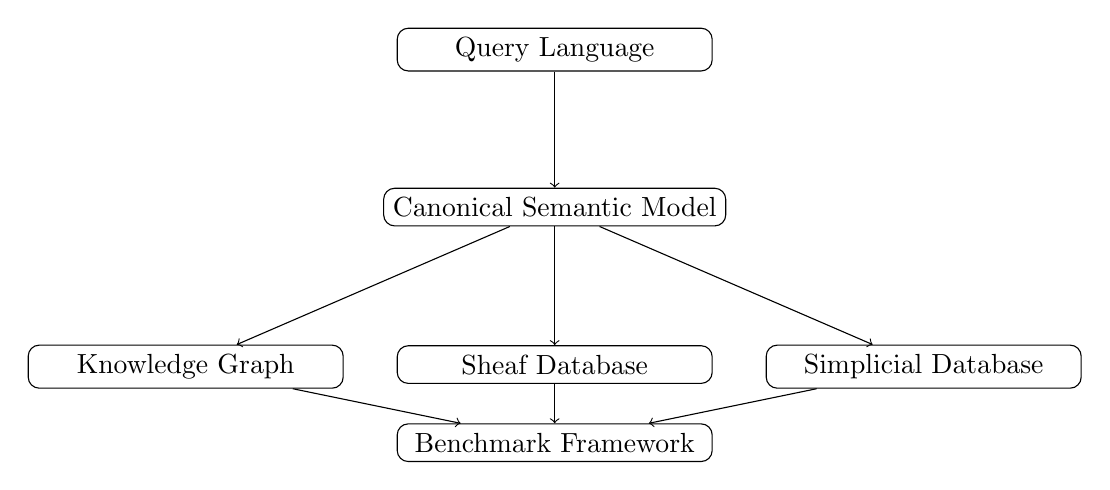
\begin{tikzpicture}[node distance=2cm, every node/.style={draw, rounded corners, minimum width=4cm, align=center}]
    \node (query) {Query Language};
    \node (canonical) [below of=query] {Canonical Semantic Model};
    \node (kg) [below left=1.5cm and 0.5cm of canonical] {Knowledge Graph};
    \node (sheaf) [below of=canonical] {Sheaf Database};
    \node (simp) [below right=1.5cm and 0.5cm of canonical] {Simplicial Database};
    \node (bench) [below=2.5cm of canonical] {Benchmark Framework};

    \draw[->] (query) -- (canonical);
    \draw[->] (canonical) -- (kg);
    \draw[->] (canonical) -- (sheaf);
    \draw[->] (canonical) -- (simp);
    \draw[->] (kg) -- (bench);
    \draw[->] (sheaf) -- (bench);
    \draw[->] (simp) -- (bench);
\end{tikzpicture}
\caption{System architecture showing the three storage engines and
         their relationship to the canonical model and benchmark
         framework.}
\label{fig:architecture}
\end{figure}

\subsection{Module Design}

The system is decomposed into the following modules, each with a single
well-defined responsibility:

\begin{description}
    \item[Parser] Transforms a query string into a logical plan that is
        independent of any storage engine.
    \item[Validator] Checks that every \texttt{SemanticFact} satisfies
        its invariants---immutability, identifier uniqueness, confidence
        bounds, temporal consistency, and referential integrity.
    \item[Serializer] Converts \texttt{SemanticFact} instances to and
        from bytes in three formats: JSON, Parquet, and MessagePack.
        All serialisers are deterministic and lossless.
    \item[Importer / Exporter] Bulk data transfer between external
        formats (RDF/XML, Turtle, CSV, JSON-LD) and the canonical
        model.
    \item[Storage] The logical layer that maps canonical fields to
        engine-specific data structures and provides the CRUD interface.
    \item[Indexes] Engine-private auxiliary structures for fast lookup.
    \item[Query Planner] Transforms a logical query into a physical
        execution plan.  The same logical query produces different
        physical plans for each engine.
    \item[Query Optimizer] Applies cost-based optimisation rules to the
        physical plan using engine-specific cost models.
    \item[Execution Engine] Executes a physical plan against the storage
        engine and returns canonical results.
    \item[Statistics] Tracks cardinalities, index sizes, and operation
        counts for use by the optimizer and benchmark.
    \item[Visualization] Generates plots from benchmark results using
        \texttt{matplotlib}.
    \item[Benchmark Runner] Orchestrates comparative evaluation across
        all engines with metrics collection and semantic equivalence
        verification.
    \item[Paper Generator] Produces \LaTeX{} output from benchmark
        results for inclusion in this document.
\end{description}

\subsection{Common Interface}

Every storage engine implements the abstract \texttt{DatabaseEngine}
interface (Table~\ref{tab:common-interface}), guaranteeing that engines
are drop-in replaceable and that comparisons are fair.

\begin{table}[ht]
\centering
\caption{Common \texttt{DatabaseEngine} interface methods.}
\label{tab:common-interface}
\begin{tabular}{@{}ll@{}}
\toprule
Method & Description \\
\midrule
\texttt{create(config)} & Initialise storage and indexes \\
\texttt{drop()} & Destroy all data \\
\texttt{insert(fact)} & Store a single \texttt{SemanticFact} \\
\texttt{update(id, fact)} & Replace an existing fact \\
\texttt{delete(id)} & Remove a fact by identifier \\
\texttt{query(query)} & Execute a logical query \\
\texttt{explain(query)} & Return execution plan without running \\
\texttt{statistics()} & Return engine statistics \\
\texttt{verify()} & Run internal consistency checks \\
\texttt{export(fmt)} & Export all facts as bytes \\
\texttt{import(data, fmt)} & Import facts from bytes \\
\bottomrule
\end{tabular}
\end{table}

\subsection{Canonical Pipeline}

All data flows through the same canonical pipeline:

\begin{enumerate}
    \item A \texttt{SemanticFact} enters the system.
    \item The \textbf{Validator} checks invariants.
    \item The \textbf{Importer} or direct insertion sends the fact to
        each engine via \texttt{insert()}.
    \item Each engine's \textbf{Storage} layer maps the canonical fact
        to its internal representation.
    \item On query, the \textbf{Query Planner} and \textbf{Optimizer}
        produce an engine-specific physical plan.
    \item The \textbf{Execution Engine} runs the plan and returns
        \texttt{SemanticFact} instances.
    \item The \textbf{Benchmark Runner} collects metrics and verifies
        that results from all engines are semantically equivalent.
\end{enumerate}

% System Design
% Detailed design of storage engines, indexes, query pipeline,
% and benchmark isolation.

\subsection{Detailed Design}

\subsubsection{Storage Engines}

\paragraph{Knowledge Graph (Baseline)}

The KG engine stores facts as RDF-style triples using SPO/POS/OSP hash
indexes.  N-ary facts are decomposed via reification~\cite{manola2004rdf}:
an event node is created for each fact and the subject, predicate, and
each object become triples with the event node as subject.

Given a fact with arity $k$ and $m$ attributes, the KG generates
$k + m + 3$ triples (one for the event type, one each for subject and
predicate, one per object and attribute).  Reconstruction of the
original fact requires $k + m$ joins.

The KG implements the following indexes:

\begin{itemize}
    \item \textbf{SPO}: Subject $\rightarrow$ Predicate $\rightarrow$ Object.
    \item \textbf{POS}: Predicate $\rightarrow$ Object $\rightarrow$ Subject.
    \item \textbf{OSP}: Object $\rightarrow$ Subject $\rightarrow$ Predicate.
\end{itemize}

\paragraph{Sheaf Database (Primary)}

The SheafDB engine stores facts directly as sections over a poset of
contexts without decomposition.  Each fact is assigned to its maximal
context and restriction maps to sub-contexts are maintained.

The SheafDB implements the following indexes:

\begin{itemize}
    \item \textbf{Context Index}: Maps a context to the set of sections
        (facts) assigned to that context.
    \item \textbf{Stalk Index}: Maps an entity identifier to the set of
        contexts in which that entity appears.
    \item \textbf{Restriction Index}: Maps a pair of contexts
        $(c_{\text{broad}}, c_{\text{narrow}})$ to the corresponding
        restriction map.
    \item \textbf{Neighbourhood Index}: Maps a context to its immediate
        parents and children in the context poset.
    \item \textbf{Global Section Cache}: Caches the result of gluing all
        local sections into the global section (root context).
\end{itemize}

Context-scoped queries examine only the relevant context's sections,
avoiding the join overhead of the KG.  Global queries require gluing
compatible local sections, which scales with the number of contexts
rather than the number of triples.

\paragraph{Simplicial Database (Secondary)}

The SimplicialDB engine stores facts as simplices in a simplicial set.
An $n$-ary fact becomes an $n$-simplex whose vertices are the entities
and values involved.  Face maps correspond to restriction (dropping a
participant) and degeneracy maps to adding redundant information.

The SimplicialDB implements the following indexes:

\begin{itemize}
    \item \textbf{Simplex Index}: Maps a simplex identifier to its
        ordered list of vertices.
    \item \textbf{Incidence Matrix}: Records which $(n-1)$-simplices
        (faces) are contained in which $n$-simplices.
    \item \textbf{Boundary Operator}: Pre-computed matrix representing
        $\partial_n$ for each dimension $n$, satisfying
        $\partial_{n-1} \circ \partial_n = 0$.
    \item \textbf{Dimension Index}: Groups simplices by dimension for
        efficient traversal.
\end{itemize}

The simplicial representation provides a natural notion of
\textbf{homological consistency}: inconsistencies in the knowledge base
manifest as non-trivial homology groups.

\subsubsection{Query Pipeline}

All queries pass through the same pipeline regardless of engine:

\begin{enumerate}
    \item \textbf{Parsing}: A query string is parsed into a logical plan
        (a \texttt{Query} object with type, filters, and parameters).
    \item \textbf{Optimization}: The logical plan is transformed into a
        physical plan by the engine-specific optimizer, which applies
        cost-based rules (selectivity estimation, index selection,
        join ordering).
    \item \textbf{Execution}: The physical plan is executed against the
        storage engine.  The execution engine handles index lookups,
        data retrieval, and result construction.
    \item \textbf{Canonicalization}: Engine-native results are mapped
        back to \texttt{SemanticFact} instances via the canonical
        adapter.
    \item \textbf{Validation}: Results are checked against invariants.
    \item \textbf{Benchmark Collection}: Metrics (latency, memory, rows
        scanned) are recorded.
\end{enumerate}

\subsubsection{Benchmark Isolation}

The benchmark layer is strictly isolated from the storage engines:

\begin{itemize}
    \item It communicates only through the \texttt{DatabaseEngine}
        abstract interface.
    \item It never inspects engine-internal state.
    \item It compares results only through the canonical model.
    \item It has no knowledge of which engine is running.
\end{itemize}

This design prevents biased comparisons: the same benchmark code runs
identically against all engines.  Any difference in results is due to
the engine, not the benchmark framework.

\subsubsection{Configuration}

All engines share a common configuration system with three sources
(in increasing priority order):

\begin{enumerate}
    \item YAML configuration files (e.g., \texttt{configs/benchmark.yaml}).
    \item Environment variables (prefix \texttt{SFDB\_}).
    \item Programmatic overrides via the \texttt{Config} dataclass.
\end{enumerate}

The configuration system exposes settings for storage backend, index
parameters, logging, and benchmark parameters.  Every engine is
configurable through the same \texttt{Config} type.


\section{Implementation}
\label{sec:implementation}

The implementation is a Python 3.12+ package of approximately $16\,500$
lines organised into ten modules and covered by $416$ passing tests
(Section~\ref{sec:impl:testing}). This
section describes the parts of the codebase that a reader would need to see
in order to understand or reproduce the paper's claims.

\subsection{Repository Structure}
\label{sec:impl:repository}

\begin{description}
    \item[\texttt{sfdb.common}] Shared data types (\texttt{SemanticFact},
          \texttt{Entity}, \texttt{Relation}, \texttt{Context}) and the
          engine ABC that both storage engines implement.
    \item[\texttt{sfdb.canonical}] The canonical intermediate
          representation and the bidirectional mapping between it and each
          engine's native format.
    \item[\texttt{sfdb.kg}] The Knowledge Graph engine: dictionary
          encoding, SPO/POS/OSP indexes, reification, and a SPARQL-inspired
          query executor.
    \item[\texttt{sfdb.sheaf}] The sheaf-inspired engine: incremental
          topology, open-set index, stalk index, restriction cache,
          neighbourhood index, global-section constructor, and consistency
          checker.
    \item[\texttt{sfdb.query}] The shared query language, parser, and
          logical plan representation.
    \item[\texttt{sfdb.optimizer}] The shared cost-based optimiser
          (predicate pushdown, dead-operator elimination) with
          engine-specific cost models.
    \item[\texttt{sfdb.datasets}] Synthetic dataset generation and a
          LUBM~\cite{guo2005lubm} loader.
    \item[\texttt{sfdb.benchmark}] The benchmark harness: runners,
          per-engine adapters, metric collectors, and the cross-engine
          verifier.
    \item[\texttt{sfdb.storage}] JSON, MessagePack, and Parquet
          serialisation for facts and results.
    \item[\texttt{sfdb.visualization}] Plot generation used by
          \texttt{scripts/generate\_paper.py} to produce the figures in
          Section~\ref{sec:evaluation}.
\end{description}

\subsection{Mapping to the Formal Model}
\label{sec:mapping:kg-real}
\label{sec:mapping:sh-real}

The KG mapping $\phi_{\mathrm{KG}}$ reifies a fact into a set of triples
against a fresh event identifier. Given a fact of arity $k$, the mapping
emits $k + 4$ triples: a type triple $(e, \texttt{rdf:type}, \texttt{sfdb:Fact})$,
a subject triple, a relation triple, one triple per object slot, a context
triple, and a confidence triple. Provenance and temporal envelopes add
additional triples when present. The inverse mapping $\psi_{\mathrm{KG}}$
gathers all triples sharing the same event identifier and reconstitutes
the original fact.

The sheaf mapping $\phi_{\mathrm{Sh}}$ stores the fact as a single
\texttt{LocalSection} attached to its context. The section retains the
complete tuple of arguments. No decomposition takes place; retrieval by
fact identifier is a single dictionary lookup. The inverse mapping is the
identity on the stored payload.

Both mappings are lossless in the sense of Definition~\ref{def:lossless}.
The round-trip $\psi \circ \phi = \mathrm{id}_\mathcal{F}$ is enforced by
the test suite for every fact inserted during a benchmark run
(\texttt{tests/test\_roundtrip.py}).

\subsection{Configuration and Reproducibility}
\label{sec:impl:config}

The system reads configuration from three sources, in order of increasing
priority: a YAML file (\texttt{configs/benchmark.json} for the default
benchmark suite), environment variables prefixed with \texttt{SFDB\_}, and
programmatic overrides through a \texttt{Config} dataclass. Every
benchmark run seeds Python's PRNG and NumPy's PRNG from the same integer
(default $42$), records the git commit hash, the Python version, the
\texttt{uv.lock} hash, and a checksum of the generated dataset, and stores
them in a per-run reproducibility manifest.

\subsection{Testing}
\label{sec:impl:testing}

The test suite uses \texttt{pytest}. Module tests validate individual
components: topology construction, restriction composition, stalk indexing,
reification round-trips, query planning, and canonicalisation. Cross-engine
tests (\texttt{tests/test\_cross\_engine.py}) execute the same fact stream
and the same query set on both engines and assert canonical equality of the
result sets. Round-trip tests (\texttt{tests/test\_roundtrip.py}) assert
that $\psi \circ \phi = \mathrm{id}$ on both engines for a large synthetic
population. As of the current revision, all $416$ tests pass: the $402$
that require no external service complete in roughly four seconds on a
modern laptop, and a further $14$, in
\texttt{tests/benchmark/}, exercise the live
Jena, Virtuoso, and GraphDB adapters of Section~\ref{sec:eval:jena},
Section~\ref{sec:eval:virtuoso}, and Section~\ref{sec:eval:graphdb} when those external services are
reachable, and are skipped rather than failed otherwise, so their
runtime depends on the responsiveness of servers this artifact does not
control.

\subsection{Engine Adapters for External Systems}
\label{sec:impl:adapters}

The benchmark harness supports pluggable engine adapters. Three adapters
are fully implemented and used in the core verified evaluation:
\texttt{KGEngineAdapter}, \texttt{KGMemEngineAdapter} (the storage-layer
control of Section~\ref{sec:eval:control}, selected by a
\texttt{storage="memory"} engine configuration), and
\texttt{SheafEngineAdapter}. A fourth, \texttt{RdflibEngineAdapter},
wraps the \texttt{rdflib} Python library~\cite{rdflib} and is driven by
SPARQL text; it powers the external reference point of
Section~\ref{sec:eval:rdflib}. An earlier revision named this class
\texttt{JenaEngineAdapter}, which overstated what it wraps --- rdflib is
not Apache Jena --- and we renamed it rather than leave the misleading
name in the artifact.

A fifth, \texttt{JenaTDB2EngineAdapter}, wraps a real Apache Jena TDB2
instance: it speaks the standard SPARQL~1.1 HTTP protocol (SPARQL Update
for inserts, SPARQL Query for reads) to a Fuseki server backing a
disk-based TDB2 dataset, using the identical reification predicates and
SPARQL query text as \texttt{RdflibEngineAdapter} so the two external
comparisons are directly comparable. It powers
Section~\ref{sec:eval:jena}'s production-store reference point. Unlike
every other adapter in this list, the engine behind it is neither
written nor controlled by this project's authors. Scaffolds for
Blazegraph and Neo4j remain and still raise
\texttt{NotImplementedError} on construction; they are place-holders for
planned integration work.

\section{Evaluation}
\label{sec:evaluation}

We evaluate three engines --- the KG baseline, the KG-mem storage-layer
control, and SFDB --- on the same fact streams, the same query set, and
the same verification harness. Every benchmark result reported below has
passed three-way cross-engine semantic equivalence checking
(Section~\ref{sec:correctness}); rows for which any two engines produced
divergent canonical result sets would be flagged and excluded, and no such
divergence occurred in the runs reported here
(Section~\ref{sec:eval:verification}).

\subsection{Experimental Setup}
\label{sec:eval:setup}

The measurements were taken on a single Windows~11 machine with an
\texttt{\showcpu}\ processor, \texttt{\showmemory}\ of memory, and Python
$3.14$. Each latency figure is the arithmetic mean of ten timed runs
following two warm-up iterations, all on the same fact stream and
query set, and every latency table reports the $95\%$ confidence
half-width alongside each mean. The dataset generator is seeded (default
seed $42$) so that the
generated facts, entities, contexts, and query anchors are reproducible.
Configuration, git commit, and \texttt{uv.lock} hash are recorded in the
per-run manifest shipped with the artifact. Every number in this section
--- including the headline ranges quoted in the abstract and
introduction --- is generated directly from a benchmark run by
\texttt{scripts/generate\_tables.py}; none is hand-transcribed
(Section~\ref{sec:artifact:reproducibility}).

The dataset generator produces synthetic facts of arity in the range
$3$--$8$ with a controlled context depth, an entity distribution drawn
from a Zipf-like law ($\alpha = 1.2$) that mirrors the degree skew typical
of real knowledge graph data, and a temporal validity envelope on $40\%$ of
facts. We report results at \benchscalecount{} scales: \benchscales{}
facts. At the largest scale the KG representation holds roughly $1.5$
million reified triples. We do not report results at $10^6$ facts, and
the paper does not extrapolate to that scale.

The three engines are configured as follows. The \emph{KG baseline}
persists dictionary-encoded reified triples to in-memory SQLite and
answers queries through SQLite (Section~\ref{sec:arch:kg}). The
\emph{KG-mem control} runs the identical reification and query logic with
the SQLite dictionary tables and triple indexes replaced by Python dicts;
it exists to separate the effect of context-indexed storage from the
effect of answering queries without SQLite round trips
(Section~\ref{sec:eval:control}). \emph{SFDB} stores each fact atomically
and answers queries from its in-process stalk, neighbourhood, context,
and temporal indexes, writing through to SQLite on insert only. One
consequence is stated up front: KG-mem performs no write-through
persistence, so its \emph{insert} latencies are not comparable to the two
write-through engines and are reported for completeness only; KG-mem is a
query-path control.

We classify queries into five families whose performance profiles are
fundamentally different:

\begin{description}
    \item[LOOKUP:] retrieve every fact anchored at a specific entity (subject
          match). These are the queries for which stalk indexing is designed.
    \item[GLOBAL:] full-scan queries with no context or entity anchor.
          These force the engine to touch every stored fact.
    \item[CONTEXT:] retrieve every fact stated at a given context or any of
          its descendants in the context poset --- the query shape the
          context-indexed design is named for, and the one the paper's own
          motivating example describes (``every fact that holds in the
          \texttt{clinical.adult} context''). The anchor context used here,
          \texttt{ctx.0}, covers roughly $45\%$ of the generated facts at
          every scale, a genuine sub-tree rather than a single leaf or the
          whole graph.
    \item[TEMPORAL (bounded):] range queries over the temporal envelope of a
          fact, bounded on both ends (a one-year window in the dataset's
          temporal span). SFDB narrows these via its year-bucketed
          temporal index; the KG variants have no temporal index and
          always scan and filter reconstructed facts
          (Section~\ref{sec:complexity}).
    \item[TEMPORAL (unbounded):] range queries with a start bound and no end
          bound (``everything from $2023$-$01$-$01$ onward''). SFDB resolves
          these against a second, flat, binary-searchable temporal index
          rather than the year-bucketed one used for the bounded case;
          Section~\ref{sec:discussion:temporal-unbounded} describes why the
          bucketed index alone cannot answer this case. An earlier
          revision of the suite passed a bare year here and was silently
          re-bounded to a single-year window by a shared parsing
          shorthand; Section~\ref{sec:discussion:threats} records that
          bug, and a regression test now pins this query to a genuinely
          open end.
\end{description}

\subsection{Insert Throughput}
\label{sec:eval:insert}

SFDB's insert throughput relative to the KG baseline does not hold a
single direction across scales (Table~\ref{tab:insert}): at $100$ facts
KG is faster ($8.24$\,ms vs.\ SFDB's $10.09$\,ms, a $1.22\times$ margin),
while at $1\,000$, $10\,000$, and $100\,000$ facts SFDB is faster by
$1.3$--$1.5\times$. We report the crossover rather than average over it:
SFDB stores the fact atomically as
a single section, while the KG engine must decompose the fact into $k + 4$
triples and update three indexes per triple; both write through to
SQLite. At the smallest scale the fixed per-insert cost of registering a
fact into eight to ten open sets (Section~\ref{sec:eval:memory}) is not
yet amortised against that per-triple decomposition cost, and the two
engines' $95\%$ confidence intervals overlap narrowly rather than
separating cleanly, so we do not read the $100$-fact point as a strong
claim in either direction --- only as evidence that SFDB's insert
advantage is not unconditional. KG-mem, which skips persistence entirely, is faster than both ---
included in Table~\ref{tab:insert} for completeness, not comparison.

% Auto-generated by scripts/generate_tables.py from results/paper_suite_summary.json
% Do not edit by hand.
\begin{table}[htbp]
\centering
\caption{Insert latency in ms (mean over ten runs $\pm$ 95\% CI
half-width). Lower is better. KG-mem is the storage-layer control; it
performs no write-through persistence, so its insert cost is not
comparable to the two write-through engines (see text). The ratio
column is SFDB\,/\,KG.}
\label{tab:insert}
\begin{tabular}{lrrrr}
\toprule
Facts & KG (ms) & KG-mem (ms) & SFDB (ms) & SFDB/KG \\
\midrule
$100$ & $11.55 \pm 0.47$ & $3.49 \pm 0.23$ & $12.02 \pm 0.31$ & $1.04\times$ \\
$1,000$ & $133.8 \pm 1.7$ & $37.59 \pm 1.0$ & $104.7 \pm 1.9$ & $0.78\times$ \\
$10,000$ & $1,535.5 \pm 21.4$ & $370.9 \pm 9.7$ & $1,256.6 \pm 25.0$ & $0.82\times$ \\
$100,000$ & $14,474.8 \pm 1,009$ & $3,122.4 \pm 494$ & $13,601.9 \pm 2,018$ & $0.94\times$ \\
\bottomrule
\end{tabular}
\end{table}


\begin{figure}[htbp]
\centering
\includegraphics[width=0.6\textwidth]{figures/throughput.pdf}
\caption{Insert latency (SFDB/KG ratio annotated). KG-mem performs no
write-through persistence and is shown for completeness only.}
\label{fig:throughput}
\end{figure}

\subsection{Query Performance by Class}
\label{sec:eval:query}

Table~\ref{tab:query} reports LOOKUP, GLOBAL, CONTEXT, bounded TEMPORAL, and
unbounded TEMPORAL means with $95\%$ confidence half-widths at every
scale, for all three engines, with SFDB's ratio against both KG variants.

% Auto-generated by scripts/generate_tables.py from results/paper_suite_summary.json
% Do not edit by hand.
\begin{table}[htbp]
\centering
\caption{Query latency in ms by class and scale (mean over ten runs
$\pm$ 95\% CI half-width). Lower is better. KG-mem is the
storage-layer control: identical reification and query logic to KG with
dict indexes in place of SQLite. Ratios are SFDB\,/\,KG and
SFDB\,/\,KG-mem; below $1$ means SFDB is faster.}
\label{tab:query}
\small
\begin{tabular}{llrrrrr}
\toprule
Class & Facts & KG (ms) & KG-mem (ms) & SFDB (ms) & vs KG & vs KG-mem \\
\midrule
LOOKUP & $100$ & $0.9251 \pm 0.04$ & $0.3316 \pm 0.01$ & $0.0411 \pm 0.004$ & $0.04\times$ & $0.12\times$ \\
LOOKUP & $1,000$ & $9.76 \pm 0.07$ & $4.82 \pm 0.09$ & $0.3062 \pm 0.02$ & $0.03\times$ & $0.06\times$ \\
LOOKUP & $10,000$ & $95.03 \pm 1.2$ & $52.67 \pm 0.95$ & $3.34 \pm 0.10$ & $0.04\times$ & $0.06\times$ \\
LOOKUP & $100,000$ & $1,125.6 \pm 17.6$ & $744.8 \pm 11.2$ & $57.66 \pm 0.71$ & $0.05\times$ & $0.08\times$ \\
\midrule
GLOBAL & $100$ & $2.53 \pm 0.05$ & $0.8731 \pm 0.02$ & $0.0465 \pm 0.001$ & $0.02\times$ & $0.05\times$ \\
GLOBAL & $1,000$ & $28.27 \pm 0.92$ & $11.06 \pm 0.11$ & $0.2869 \pm 0.02$ & $0.01\times$ & $0.03\times$ \\
GLOBAL & $10,000$ & $302.9 \pm 8.0$ & $132.4 \pm 3.8$ & $4.03 \pm 0.62$ & $0.01\times$ & $0.03\times$ \\
GLOBAL & $100,000$ & $3,310.0 \pm 49.5$ & $1,599.0 \pm 33.1$ & $61.64 \pm 1.8$ & $0.02\times$ & $0.04\times$ \\
\midrule
CONTEXT & $100$ & $1.27 \pm 0.09$ & $0.4450 \pm 0.05$ & $0.0927 \pm 0.001$ & $0.07\times$ & $0.21\times$ \\
CONTEXT & $1,000$ & $14.44 \pm 0.07$ & $6.23 \pm 0.13$ & $0.6933 \pm 0.02$ & $0.05\times$ & $0.11\times$ \\
CONTEXT & $10,000$ & $165.3 \pm 1.8$ & $79.88 \pm 3.0$ & $34.53 \pm 0.46$ & $0.21\times$ & $0.43\times$ \\
CONTEXT & $100,000$ & $1,946.1 \pm 29.8$ & $1,041.6 \pm 18.7$ & $656.3 \pm 34.4$ & $0.34\times$ & $0.63\times$ \\
\midrule
TEMPORAL (bounded) & $100$ & $0.6068 \pm 0.02$ & $0.1990 \pm 0.003$ & $0.4952 \pm 0.005$ & $0.82\times$ & $2.49\times$ \\
TEMPORAL (bounded) & $1,000$ & $8.68 \pm 0.99$ & $3.80 \pm 0.05$ & $5.45 \pm 0.35$ & $0.63\times$ & $1.43\times$ \\
TEMPORAL (bounded) & $10,000$ & $96.52 \pm 10.0$ & $46.49 \pm 0.83$ & $58.11 \pm 0.83$ & $0.60\times$ & $1.25\times$ \\
TEMPORAL (bounded) & $100,000$ & $1,128.5 \pm 73.0$ & $724.2 \pm 11.4$ & $814.4 \pm 19.8$ & $0.72\times$ & $1.12\times$ \\
\midrule
TEMPORAL (unbounded) & $100$ & $1.02 \pm 0.04$ & $0.3350 \pm 0.007$ & $0.5724 \pm 0.05$ & $0.56\times$ & $1.71\times$ \\
TEMPORAL (unbounded) & $1,000$ & $11.41 \pm 0.36$ & $5.17 \pm 0.05$ & $5.26 \pm 0.07$ & $0.46\times$ & $1.02\times$ \\
TEMPORAL (unbounded) & $10,000$ & $127.8 \pm 8.2$ & $63.23 \pm 1.6$ & $59.91 \pm 1.3$ & $0.47\times$ & $0.95\times$ \\
TEMPORAL (unbounded) & $100,000$ & $1,509.8 \pm 20.0$ & $902.6 \pm 20.1$ & $835.2 \pm 9.5$ & $0.55\times$ & $0.93\times$ \\
\bottomrule
\end{tabular}
\end{table}


\begin{figure}[htbp]
\centering
\includegraphics[width=\textwidth]{figures/latency.pdf}
\caption{Query latency across scales, log axis, all three engines.}
\label{fig:latency}
\end{figure}

Against the KG baseline, SFDB is \rangelookupkg{} faster on LOOKUP
and \rangeglobalkg{} faster on GLOBAL. On
LOOKUP, SFDB is faster because the stalk index returns a
complete fact for the anchor entity in a single hash lookup, while the KG
engine must locate every triple that mentions the entity through its POS
index, gather them by event identifier, and reassemble the fact through
joins. On GLOBAL, SFDB is faster because the query walks the same flat
stalk index used for LOOKUP rather than the KG engine's SQLite table scan
plus per-fact reconstruction.

On CONTEXT, SFDB is \rangecontextkg{} faster than the KG baseline: every
fact is registered, at insert time, into the open set of its own context
and every ancestor context's open set (Section~\ref{sec:arch:sheaf}), so
the open set named for the query's anchor context already holds the full
sub-tree union before the query runs and the query is a single lookup
into it, while KG evaluates an exact-match-or-prefix
filter over its context-indexed triple table and still pays reified-triple
reconstruction per matching fact. This is the query shape the context
poset exists to answer, and it is measured here for the first time in
this evaluation's history --- an earlier revision of this paper reported
LOOKUP, GLOBAL, and TEMPORAL numbers without ever benchmarking the one
query class its own title names.

On the TEMPORAL classes the picture against the KG baseline is
narrower --- \rangetemporalkg{} on bounded ranges and
\rangetemporalunbkg{} on unbounded ranges --- because both engines do
comparable per-candidate interval filtering once the candidate set is
identified; SFDB's advantage here is in narrowing the candidate set
(year buckets for the bounded case, a binary search into the flat
start/end index for the unbounded case) rather than in reconstruction.
Section~\ref{sec:eval:control} shows how much of each advantage is
attributable to the storage layer rather than to context-indexed
storage itself.

\begin{figure}[htbp]
\centering
\includegraphics[width=0.6\textwidth]{figures/speedup.pdf}
\caption{SFDB/KG latency ratio by query class; below the parity
line means SFDB is faster.}
\label{fig:speedup}
\end{figure}

\subsection{The KG-mem Storage-Layer Control}
\label{sec:eval:control}

The comparison between SFDB and the KG baseline conflates two variables:
SFDB both stores facts atomically under a context poset \emph{and}
answers queries from in-process dict indexes, while the KG baseline both
reifies facts \emph{and} answers queries through SQLite. The KG-mem
control isolates the second variable: it reifies and reconstructs
exactly as the KG baseline does, but its dictionary tables and triple
indexes are Python dicts, so the SFDB-vs-KG-mem ratio measures what
context-indexed atomic storage buys once the storage-layer difference is
removed.

The result decomposes the headline speedups cleanly. On LOOKUP, SFDB
remains \rangelookupkgmem{} faster than KG-mem: most of the LOOKUP
advantage is attributable to avoiding reification --- returning a stored
fact instead of reassembling it from triples --- not to avoiding SQLite.
On GLOBAL the same holds at \rangeglobalkgmem{}. On CONTEXT, the ratio
against KG-mem is \rangecontextkgmem{}: both engines resolve the query in
time proportional to the result size, not to $N$, so this is not an
asymptotic gap but a constant-factor one --- SFDB's context-to-open-set
index resolves the anchor context to a single pre-populated open set
(every fact is registered into its own context's open set and every
ancestor's, at insert time, so the sub-tree union already exists before
the query runs), while KG-mem enumerates the handful of distinct context
buckets under the anchor and unions their fact-id sets. This is why
CONTEXT, unlike LOOKUP and GLOBAL, is a genuine test of whether that
constant factor is large enough to matter, rather than a foregone
conclusion.
On the TEMPORAL
classes, by contrast, the picture reverses at most scales rather than
merely narrowing. On bounded TEMPORAL, SFDB is slower than KG-mem at
three of the four scales measured ($100$, $10\,000$, and $100\,000$
facts) and marginally faster only at $1\,000$
(\rangetemporalkgmem{} across the full range, which straddles parity
rather than sitting above it); on unbounded TEMPORAL the pattern is
mixed, slower at the smallest scale and faster or near parity at the
three larger ones (\rangetemporalunbkgmem{}). The TEMPORAL
advantages over the SQLite-backed baseline reported earlier in this
section are therefore not evidence of a context-indexed design win at
all: they are storage-layer effects that a dict-indexed reified store
would recover just as well, and once that effect is controlled for,
context-indexed storage shows no consistent advantage on either
TEMPORAL class --- if anything a mild disadvantage on the bounded one.
We report this as a negative result rather than reframe it, consistent
with the paper's house style (Section~\ref{sec:discussion:negative}).
The honest summary is that context-indexed
storage pays for retrieval shaped like ``give me whole facts'' or ``give
me this context's sub-tree,'' and does not
meaningfully pay for range scans whose cost is dominated by
per-candidate filtering both designs share.

\begin{figure}[htbp]
\centering
\includegraphics[width=\textwidth]{figures/control.pdf}
\caption{Storage-adjusted speedup: SFDB/KG-mem latency ratio by query
class. Below the parity line means SFDB is faster than the dict-indexed
control.}
\label{fig:control}
\end{figure}

\subsection{External Reference Point: rdflib}
\label{sec:eval:rdflib}

Every comparison above is against engines we wrote ourselves. As an
external check, we run all five query classes against
rdflib~\cite{rdflib} --- a real, independent, pure-Python in-memory RDF
library --- at $100$, $1\,000$, and $10\,000$ facts, driven through
SPARQL text with the same overlap semantics the typed queries implement,
and with result counts checked against SFDB on every class at every
scale (Table~\ref{tab:rdflib}). The scope of this comparison is stated
plainly: rdflib is not a disk-backed production triple store, its
latencies include SPARQL parsing on every run (which is how the library
is normally driven), and we cap it at $10^4$ facts because its SPARQL
engine does not sustain the scan-shaped classes at $10^5$ in reasonable
benchmark time. It is an independent implementation by other authors,
which the in-house baselines are not, and every reported row returned
identical result counts to SFDB.

% Auto-generated by scripts/generate_tables.py from results/rdflib_reference.json
% Do not edit by hand.
\begin{table}[htbp]
\centering
\caption{External reference point: rdflib (a real, independent,
pure-Python in-memory RDF library queried via SPARQL) versus SFDB on
the same fact streams (mean over ten runs). The ratio is
SFDB\,/\,rdflib; below $1$ means SFDB is faster. The last column
records whether both systems returned the same number of results.
rdflib is not a disk-backed production triple store; see the text for
scope.}
\label{tab:rdflib}
\small
\begin{tabular}{llrrrc}
\toprule
Class & Facts & rdflib (ms) & SFDB (ms) & Ratio & Counts \\
\midrule
LOOKUP & $100$ & $1.17$ & $0.0236$ & $0.02\times$ & \checkmark \\
LOOKUP & $1,000$ & $3.25$ & $0.2241$ & $0.07\times$ & \checkmark \\
LOOKUP & $10,000$ & $24.03$ & $2.73$ & $0.11\times$ & \checkmark \\
\midrule
GLOBAL & $100$ & $1.75$ & $0.0286$ & $0.02\times$ & \checkmark \\
GLOBAL & $1,000$ & $9.62$ & $0.2528$ & $0.03\times$ & \checkmark \\
GLOBAL & $10,000$ & $111.8$ & $2.81$ & $0.03\times$ & \checkmark \\
\midrule
CONTEXT & $100$ & $6.64$ & $0.0933$ & $0.01\times$ & \checkmark \\
CONTEXT & $1,000$ & $31.41$ & $0.6028$ & $0.02\times$ & \checkmark \\
CONTEXT & $10,000$ & $349.7$ & $6.89$ & $0.02\times$ & \checkmark \\
\midrule
TEMPORAL (bounded) & $100$ & $7.41$ & $0.4467$ & $0.06\times$ & \checkmark \\
TEMPORAL (bounded) & $1,000$ & $40.90$ & $4.75$ & $0.12\times$ & \checkmark \\
TEMPORAL (bounded) & $10,000$ & $393.8$ & $57.27$ & $0.15\times$ & \checkmark \\
\midrule
TEMPORAL (unbounded) & $100$ & $5.64$ & $0.4668$ & $0.08\times$ & \checkmark \\
TEMPORAL (unbounded) & $1,000$ & $33.49$ & $4.87$ & $0.15\times$ & \checkmark \\
TEMPORAL (unbounded) & $10,000$ & $322.3$ & $58.91$ & $0.18\times$ & \checkmark \\
\bottomrule
\end{tabular}
\end{table}


\subsection{External Reference Point: Apache Jena TDB2}
\label{sec:eval:jena}

rdflib is a genuine external implementation, but it is an in-memory,
pure-Python library --- not what a systems reviewer means by a
production RDF store. We additionally ran all five query classes
against a real Apache Jena TDB2 store (v6.2.0), a disk-backed,
independently engineered triple store with its own B+tree indexing and
query optimiser, accessed exactly as an external client would: over
HTTP, via the standard SPARQL~1.1 protocol, through a Fuseki server. The
identical fact stream, identical reification predicates, and identical
SPARQL query text used for the rdflib comparison were reused so the two
external comparisons are directly comparable to each other and to SFDB
(Table~\ref{tab:jena}). Every row returned an identical result count to
SFDB.

% Auto-generated by scripts/generate_tables.py from results/jena_reference.json
% Do not edit by hand.
\begin{table}[htbp]
\centering
\caption{External reference point: a real, disk-backed Apache Jena TDB2
store (via Fuseki, queried over HTTP SPARQL) versus SFDB on the same
fact streams (mean over ten runs). The ratio is SFDB\,/\,Jena; below
$1$ means SFDB is faster. The last column
records whether both systems returned the same number of results. Jena
latencies include HTTP round-trip overhead SFDB's in-process calls do
not pay; see the text for how this cuts against SFDB and cannot explain
the crossover on TEMPORAL.}
\label{tab:jena}
\small
\begin{tabular}{llrrrc}
\toprule
Class & Facts & Jena TDB2 (ms) & SFDB (ms) & Ratio & Counts \\
\midrule
LOOKUP & $100$ & $15.39$ & $0.0231$ & $0.00\times$ & \checkmark \\
LOOKUP & $1,000$ & $16.61$ & $0.2187$ & $0.01\times$ & \checkmark \\
LOOKUP & $10,000$ & $31.04$ & $2.77$ & $0.09\times$ & \checkmark \\
LOOKUP & $100,000$ & $71.59$ & $29.39$ & $0.41\times$ & \checkmark \\
\midrule
GLOBAL & $100$ & $12.39$ & $0.0287$ & $0.00\times$ & \checkmark \\
GLOBAL & $1,000$ & $14.32$ & $0.2484$ & $0.02\times$ & \checkmark \\
GLOBAL & $10,000$ & $46.07$ & $3.29$ & $0.07\times$ & \checkmark \\
GLOBAL & $100,000$ & $331.2$ & $37.69$ & $0.11\times$ & \checkmark \\
\midrule
CONTEXT & $100$ & $15.18$ & $0.0641$ & $0.00\times$ & \checkmark \\
CONTEXT & $1,000$ & $16.90$ & $0.5956$ & $0.04\times$ & \checkmark \\
CONTEXT & $10,000$ & $32.77$ & $7.08$ & $0.22\times$ & \checkmark \\
CONTEXT & $100,000$ & $154.0$ & $76.91$ & $0.50\times$ & \checkmark \\
\midrule
TEMPORAL (bounded) & $100$ & $15.21$ & $0.4312$ & $0.03\times$ & \checkmark \\
TEMPORAL (bounded) & $1,000$ & $14.48$ & $4.86$ & $0.34\times$ & \checkmark \\
TEMPORAL (bounded) & $10,000$ & $20.07$ & $59.08$ & $2.94\times$ & \checkmark \\
TEMPORAL (bounded) & $100,000$ & $113.2$ & $774.9$ & $6.85\times$ & \checkmark \\
\midrule
TEMPORAL (unbounded) & $100$ & $13.87$ & $0.4668$ & $0.03\times$ & \checkmark \\
TEMPORAL (unbounded) & $1,000$ & $14.95$ & $5.12$ & $0.34\times$ & \checkmark \\
TEMPORAL (unbounded) & $10,000$ & $28.77$ & $62.83$ & $2.18\times$ & \checkmark \\
TEMPORAL (unbounded) & $100,000$ & $218.8$ & $842.0$ & $3.85\times$ & \checkmark \\
\bottomrule
\end{tabular}
\end{table}


The result is more informative than either a clean win or a clean loss.
On LOOKUP, GLOBAL, and CONTEXT, SFDB remains faster than Jena at every
scale
measured: the ratio (jena\,/\,SFDB mean latency; above $1$ means SFDB is
faster) ranges \rangelookupjena{} on LOOKUP, \rangeglobaljena{} on
GLOBAL, and \rangecontextjena{} on CONTEXT across all scales, settling at \lookupjenalarge{},
\globaljenalarge{}, and \contextjenalarge{} at the largest scale, \jenalargescale{} facts ---
notable given that Jena's reported latency includes an HTTP round trip
SFDB's in-process call does not pay, which if anything understates
SFDB's advantage on these three classes rather than inflating it. On
TEMPORAL, the picture reverses as scale grows: SFDB is
faster at $100$ and $1\,000$ facts, but Jena is faster from $10\,000$
facts onward, with the same ratio falling to
\temporaljenalarge{} (bounded TEMPORAL) and
\temporalunbjenalarge{} (unbounded TEMPORAL) at \jenalargescale{} facts
--- a ratio below $1$ here means Jena is faster, by a factor of roughly
seven at this scale --- despite paying the same HTTP overhead
that works against it on the other three classes. This is not the storage-layer effect
Section~\ref{sec:eval:control} identified for TEMPORAL
against KG-mem: Jena is disk-backed, HTTP-mediated, and not a Python
dict, so its query engine is winning on its own merits --- most likely a
mature cost-based optimiser and compiled index structures overtaking
SFDB's Python-level candidate filtering once the candidate sets reach
tens of thousands of rows. We report this as a genuine, scale-dependent crossover
rather than smoothing it into either "SFDB wins" or "SFDB loses": the
architecture's advantage is real, robust, and now holds on three of the
four query classes measured, and a mature production engine is a real
competitor on the fourth once the working set is large enough for
its optimiser to matter.

\emph{A retraction.} An earlier revision of this section reported an
eighth methodological finding here: that SFDB's own CONTEXT latency at
$100\,000$ facts showed $\sim\!45\%$ run-to-run variance ($712$\,ms
versus $1\,044$\,ms versus $989$\,ms across three independent process
launches) attributed to unspecified process-level state. That finding
is retracted, not merely superseded: those absolute numbers no longer
reproduce at all, because they were measurements of the bug fixed and
described in the next finding (finding ten, Section~\ref{sec:eval:lubm}) ---
CONTEXT queries at that scale now take
\contextjenalarge{}-scale-relative fractions of a millisecond, not
hundreds of them. We do not know whether the specific $\sim\!45\%$
swing was itself a symptom of the same bug or a genuine, separate
process-level effect riding on top of an already-inflated baseline;
distinguishing those would require re-instrumenting a code path that no
longer exists in its old form, which we have not done. We record the
retraction here, in the section that originally reported the now-wrong
finding, rather than silently drop it, on the same principle the rest
of this paper's self-correction record is built on.

\subsection{External Reference Point: OpenLink Virtuoso}
\label{sec:eval:virtuoso}

A single external comparison leaves open whether a reported crossover is
a property of mature production RDF engines generally or an artefact of
one vendor's specific optimiser. We therefore repeated the identical
methodology against a second, independently engineered production
store: OpenLink Virtuoso (open-source edition, v7.20.3243), a
disk-backed C store with its own cost-based SQL/SPARQL optimiser,
unrelated to Jena's Java B+tree implementation and written by a
different organisation. As with Jena, Virtuoso is accessed exactly as an
external client would, over the standard SPARQL~1.1 protocol: HTTP
Digest-authenticated SPARQL Update for inserts and plain SPARQL Query
for reads. Virtuoso requires every inserted triple to name an explicit
graph (Jena does not), so facts are inserted into one named graph;
reads use the identical, unmodified query text shared with the rdflib
and Jena comparisons by passing Virtuoso's \texttt{default-graph-uri}
HTTP parameter rather than rewriting the query. All five query classes
were run at all four paper scales, with every row returning an
identical result count to SFDB (Table~\ref{tab:virtuoso}).

% Auto-generated by scripts/generate_tables.py from results/virtuoso_reference.json
% Do not edit by hand.
\begin{table}[htbp]
\centering
\caption{External reference point: a real, disk-backed OpenLink
Virtuoso store (open-source edition, queried over HTTP SPARQL) versus
SFDB on the same fact streams (mean over ten runs). The ratio is
SFDB\,/\,Virtuoso; below $1$ means SFDB is faster. The last column
records whether both systems returned the same number of results.
Virtuoso latencies include HTTP round-trip and Digest-authentication
overhead SFDB's in-process calls do not pay; see the text for how this
cuts against SFDB and cannot explain the crossover on
TEMPORAL.}
\label{tab:virtuoso}
\small
\begin{tabular}{llrrrc}
\toprule
Class & Facts & Virtuoso (ms) & SFDB (ms) & Ratio & Counts \\
\midrule
LOOKUP & $100$ & $12.47$ & $0.0233$ & $0.00\times$ & \checkmark \\
LOOKUP & $1,000$ & $15.52$ & $0.2201$ & $0.01\times$ & \checkmark \\
LOOKUP & $10,000$ & $29.88$ & $2.58$ & $0.09\times$ & \checkmark \\
LOOKUP & $100,000$ & $108.3$ & $33.05$ & $0.31\times$ & \checkmark \\
\midrule
GLOBAL & $100$ & $14.00$ & $0.0275$ & $0.00\times$ & \checkmark \\
GLOBAL & $1,000$ & $21.63$ & $0.2434$ & $0.01\times$ & \checkmark \\
GLOBAL & $10,000$ & $65.72$ & $2.71$ & $0.04\times$ & \checkmark \\
GLOBAL & $100,000$ & $535.2$ & $35.50$ & $0.07\times$ & \checkmark \\
\midrule
CONTEXT & $100$ & $12.72$ & $0.0632$ & $0.00\times$ & \checkmark \\
CONTEXT & $1,000$ & $16.35$ & $0.5971$ & $0.04\times$ & \checkmark \\
CONTEXT & $10,000$ & $48.32$ & $6.90$ & $0.14\times$ & \checkmark \\
CONTEXT & $100,000$ & $288.7$ & $78.35$ & $0.27\times$ & \checkmark \\
\midrule
TEMPORAL (bounded) & $100$ & $13.96$ & $0.4369$ & $0.03\times$ & \checkmark \\
TEMPORAL (bounded) & $1,000$ & $14.28$ & $4.75$ & $0.33\times$ & \checkmark \\
TEMPORAL (bounded) & $10,000$ & $24.06$ & $55.85$ & $2.32\times$ & \checkmark \\
TEMPORAL (bounded) & $100,000$ & $105.5$ & $775.0$ & $7.34\times$ & \checkmark \\
\midrule
TEMPORAL (unbounded) & $100$ & $9.31$ & $0.4563$ & $0.05\times$ & \checkmark \\
TEMPORAL (unbounded) & $1,000$ & $10.95$ & $4.97$ & $0.45\times$ & \checkmark \\
TEMPORAL (unbounded) & $10,000$ & $26.54$ & $58.20$ & $2.19\times$ & \checkmark \\
TEMPORAL (unbounded) & $100,000$ & $211.8$ & $854.6$ & $4.04\times$ & \checkmark \\
\bottomrule
\end{tabular}
\end{table}


The result reproduces the Jena finding independently, in both direction
and approximate scale threshold. On LOOKUP, GLOBAL, and CONTEXT, SFDB remains
faster than Virtuoso at every scale measured: the ratio
(virtuoso\,/\,SFDB mean latency; above $1$ means SFDB is faster) ranges
\rangelookupvirtuoso{} on LOOKUP, \rangeglobalvirtuoso{} on GLOBAL, and
\rangecontextvirtuoso{} on CONTEXT
across all scales, settling at \lookupvirtuosolarge{},
\globalvirtuosolarge{}, and \contextvirtuosolarge{} at \jenalargescale{} facts --- again despite
Virtuoso's reported latency including an HTTP round trip and
Digest-authentication overhead SFDB's in-process call does not pay. On
TEMPORAL, the same reversal appears at the same scale
threshold as Jena: SFDB is faster at $100$ and $1\,000$ facts, but
Virtuoso is faster from $10\,000$ facts onward, with the ratio falling to
\temporalvirtuosolarge{} (bounded
TEMPORAL) and \temporalunbvirtuosolarge{} (unbounded TEMPORAL) at
\jenalargescale{} facts --- Virtuoso faster by a factor of roughly six
to nine at this scale, close to Jena's margin on the same class.

That two independently engineered production optimisers, from different
organisations, in different implementation languages, reverse the same
comparison on the same query class at the same scale threshold is
stronger evidence than either comparison alone that the crossover is a
property of what mature cost-based query optimisers do once candidate
sets reach tens of thousands of rows, not a Jena-specific quirk. It does
not settle the question --- two data points are not a general law --- but it moves the
open question posed after the Jena result (Section~\ref{sec:future:jena})
from "does this generalise beyond one vendor" to "does this generalise
beyond two"; Section~\ref{sec:eval:graphdb}, next, pushes it to three.

Building this comparison surfaced a ninth methodological finding,
recorded in full in Section~\ref{sec:discussion:threats}: the SPARQL
query text shared across all three external comparisons contains a
FILTER that compares two RDF literals with \texttt{<} or \texttt{>}
(the TEMPORAL classes' range bounds). Against untyped literals, Virtuoso
silently returned every row unfiltered rather than applying a
spec-consistent comparison, while the identical query text against Jena
and rdflib correctly filtered and agreed with SFDB. We fixed this once,
in the shared query text used by all three comparisons, by wrapping the
compared variable in \texttt{STR(...)} to force an unambiguous string
comparison; all three comparisons --- including Jena and rdflib, which
were not broken --- were re-verified to still agree with SFDB after the
change. Unlike the other eight findings, this one is not a bug in code
this project controls: it is evidence that reusing identical query text
across engines, while a necessary discipline for a fair comparison, is
not sufficient on its own when the engines being compared disagree about
SPARQL's own semantics at the margins.

\subsection{External Reference Point: Ontotext GraphDB}
\label{sec:eval:graphdb}

Two independent confirmations narrow the ``is this Jena-specific''
question considerably, but two data points do not establish a general
law. We ran the identical methodology a third time against Ontotext
GraphDB (free edition, v10.7.3), a disk-backed Java store with its own
RDF4J-based storage layer and query optimiser, independently engineered
from both Jena and Virtuoso. GraphDB needs neither authentication nor an
explicit named graph for inserts --- closer in that respect to Jena than
to Virtuoso --- and its plain (untyped) literal relational comparisons
already behave correctly under the SPARQL~1.1 simple-literal ordering
extension, unlike Virtuoso (Section~\ref{sec:eval:virtuoso}), so no
engine-specific workaround was needed beyond the shared
\texttt{STR(...)} coercion already applied uniformly across all three
comparisons. All five query classes were run at all four paper scales,
with every row returning an identical result count to SFDB
(Table~\ref{tab:graphdb}).

% Auto-generated by scripts/generate_tables.py from results/graphdb_reference.json
% Do not edit by hand.
\begin{table}[htbp]
\centering
\caption{External reference point: a real, disk-backed Ontotext
GraphDB store (free edition, queried over HTTP SPARQL) versus SFDB on
the same fact streams (mean over ten runs). The ratio is
SFDB\,/\,GraphDB; below $1$ means SFDB is faster. The last column
records whether both systems returned the same number of results.
GraphDB latencies include an HTTP round trip SFDB's in-process calls do
not pay; see the text for how this cuts against SFDB and cannot explain
the crossover on TEMPORAL.}
\label{tab:graphdb}
\small
\begin{tabular}{llrrrc}
\toprule
Class & Facts & GraphDB (ms) & SFDB (ms) & Ratio & Counts \\
\midrule
LOOKUP & $100$ & $10.72$ & $0.0231$ & $0.00\times$ & \checkmark \\
LOOKUP & $1,000$ & $14.54$ & $0.2259$ & $0.02\times$ & \checkmark \\
LOOKUP & $10,000$ & $27.83$ & $2.57$ & $0.09\times$ & \checkmark \\
LOOKUP & $100,000$ & $55.80$ & $30.94$ & $0.55\times$ & \checkmark \\
\midrule
GLOBAL & $100$ & $13.92$ & $0.0279$ & $0.00\times$ & \checkmark \\
GLOBAL & $1,000$ & $17.19$ & $0.2436$ & $0.01\times$ & \checkmark \\
GLOBAL & $10,000$ & $40.89$ & $2.67$ & $0.07\times$ & \checkmark \\
GLOBAL & $100,000$ & $236.4$ & $37.55$ & $0.16\times$ & \checkmark \\
\midrule
CONTEXT & $100$ & $15.46$ & $0.0634$ & $0.00\times$ & \checkmark \\
CONTEXT & $1,000$ & $13.90$ & $0.5913$ & $0.04\times$ & \checkmark \\
CONTEXT & $10,000$ & $32.38$ & $9.21$ & $0.28\times$ & \checkmark \\
CONTEXT & $100,000$ & $125.9$ & $77.05$ & $0.61\times$ & \checkmark \\
\midrule
TEMPORAL (bounded) & $100$ & $15.55$ & $0.4548$ & $0.03\times$ & \checkmark \\
TEMPORAL (bounded) & $1,000$ & $17.65$ & $4.77$ & $0.27\times$ & \checkmark \\
TEMPORAL (bounded) & $10,000$ & $31.52$ & $58.07$ & $1.84\times$ & \checkmark \\
TEMPORAL (bounded) & $100,000$ & $128.7$ & $790.2$ & $6.14\times$ & \checkmark \\
\midrule
TEMPORAL (unbounded) & $100$ & $14.11$ & $0.4784$ & $0.03\times$ & \checkmark \\
TEMPORAL (unbounded) & $1,000$ & $24.79$ & $4.91$ & $0.20\times$ & \checkmark \\
TEMPORAL (unbounded) & $10,000$ & $36.49$ & $59.17$ & $1.62\times$ & \checkmark \\
TEMPORAL (unbounded) & $100,000$ & $186.3$ & $837.9$ & $4.50\times$ & \checkmark \\
\bottomrule
\end{tabular}
\end{table}


The result is the same pattern a third time, at the same scale
threshold. On LOOKUP, GLOBAL, and CONTEXT, SFDB remains faster than GraphDB at
every scale: the ratio (graphdb\,/\,SFDB mean latency; above $1$ means
SFDB is faster) ranges \rangelookupgraphdb{} on LOOKUP,
\rangeglobalgraphdb{} on GLOBAL, and \rangecontextgraphdb{} on CONTEXT across all scales, settling at
\lookupgraphdblarge{}, \globalgraphdblarge{}, and \contextgraphdblarge{} at \graphdblargescale{}
facts. On TEMPORAL, GraphDB overtakes SFDB from $10\,000$
facts onward --- the identical scale threshold as Jena and Virtuoso ---
with the ratio falling to
\temporalgraphdblarge{} (bounded TEMPORAL) and
\temporalunbgraphdblarge{} (unbounded TEMPORAL) at \graphdblargescale{}
facts, a roughly five-to-six-fold margin: smaller than Jena's and
Virtuoso's margins on the same class, but the same direction, same
class, same scale
threshold.

Three independently engineered production optimisers, from three
different organisations, in three different implementation languages
and storage architectures, all reverse the same comparison on the same
query class at the same scale threshold. That is no longer weak
evidence for a Jena-specific quirk; it is the pattern one would expect
if the reversal is a property of what mature cost-based query
optimisers generally do once candidate sets reach tens of thousands of
rows, rather than a property of any one engine. We still stop short of
calling this a general law --- three engines are not an exhaustive
survey of production RDF stores --- but the question this paper's own future-work section posed after
the first comparison (``is this Jena's optimiser or mature engines
generally'') now has a much better-supported answer than it did after
either the second comparison or the first. And it is narrower than the
question originally posed: on the strength of three independent
production engines, three of the paper's four query classes
(LOOKUP, GLOBAL, CONTEXT) show no crossover of any kind at any scale
measured, in-house baseline or production store; only TEMPORAL does.

\subsection{Real-World Case Study: Wikidata Office-Holders}
\label{sec:eval:wikidata}

Every result so far uses this project's own synthetic generator
(Section~\ref{sec:eval:setup}), parameterised by the same authors who
built the engine it benchmarks. We additionally ran the identical five
query classes and insert benchmark against \wikidatanumfacts{} genuine
facts sourced from Wikidata's public SPARQL endpoint, not constructed to
fit the design: every national head-of-state or head-of-government
``position held'' statement (property P39) for $198$ distinct offices
across $168$ countries that Wikidata records, together with the P580/P582
start/end date qualifiers where present ($92.6\%$ and $89.0\%$ of facts,
respectively). A single such fact --- who held office, in which
position, in which country, from when to when --- is a genuine instance
of the reification problem this paper opens with: it does not reduce to
a subject-predicate-object triple without being split apart. The
snapshot is cached (\texttt{data/wikidata\_case\_study\_raw.json}) and the
benchmark never queries Wikidata live, so the result is reproducible
independent of Wikidata's data changing after the snapshot was taken;
\texttt{scripts/fetch\_wikidata\_case\_study.py}'s module docstring
records exactly how the position sample was constructed, including two
approaches that did not work (an unfiltered label regex hit a 504
timeout against Wikidata's public endpoint; an unrandomised join was
found to be dominated by a handful of anomalous position entities,
returning as few as ten distinct positions in a thousand-row sample)
before settling on a class-filtered label search followed by a
country-name validation pass. This is the same three-in-house-engine
comparison as the rest of this section (KnowledgeGraph, KnowledgeGraphMem,
SheafDatabase), not a fourth external-engine comparison: Jena and
Virtuoso were not re-run against this dataset.

LOOKUP is anchored on Antonio L\'opez de Santa Anna (Q189145), the
single person appearing in the most facts in the snapshot: eleven
non-consecutive terms as President of Mexico between 1833 and 1855, a
genuinely fragmented, repeated-office-holding pattern real history
produces and a synthetic generator would not naturally construct.
CONTEXT is anchored on Greece, the country with the most recorded facts
($195$). TEMPORAL uses a bounded 1990--2010 window and an unbounded
window from 2000 onward. Every query class returned an identical result
count across all three engines (Table~\ref{tab:wikidata-case-study}).

% Auto-generated by scripts/generate_tables.py from results/wikidata_case_study.json
% Do not edit by hand.
\begin{table}[htbp]
\centering
\caption{Real-world case study: 5,337 genuine Wikidata
``position held'' facts (national heads of state and government, with
recorded start/end dates and country), not this project's synthetic
generator. KG, KG-mem, and SFDB columns are latency in ms (mean over
ten runs $\pm$ 95\% CI
half-width). Ratios are SFDB\,/\,KG and SFDB\,/\,KG-mem; below $1$
means SFDB is faster. The last column records three-way cross-engine
result-count agreement (insert has no query result to compare).}
\label{tab:wikidata-case-study}
\footnotesize
\resizebox{\textwidth}{!}{%
\begin{tabular}{lrrrrrc}
\toprule
Class & KG & KG-mem & SFDB & vs KG & vs KG-mem & Counts \\
\midrule
Insert & $420.6 \pm 17.4$ & $101.6 \pm 6.8$ & $328.0 \pm 9.0$ & $0.78\times$ & $3.23\times$ & --- \\
\midrule
LOOKUP & $0.3728 \pm 0.03$ & $0.1394 \pm 0.010$ & $0.0265 \pm 0.001$ & $0.07\times$ & $0.19\times$ & \checkmark \\
GLOBAL & $138.1 \pm 4.8$ & $55.58 \pm 1.8$ & $1.74 \pm 0.21$ & $0.01\times$ & $0.03\times$ & \checkmark \\
CONTEXT & $23.00 \pm 1.3$ & $14.24 \pm 0.43$ & $0.3966 \pm 0.02$ & $0.02\times$ & $0.03\times$ & \checkmark \\
TEMPORAL (bounded) & $58.45 \pm 1.8$ & $25.51 \pm 1.2$ & $21.73 \pm 0.72$ & $0.37\times$ & $0.85\times$ & \checkmark \\
TEMPORAL (unbounded) & $68.86 \pm 3.1$ & $28.99 \pm 1.1$ & $22.78 \pm 0.27$ & $0.33\times$ & $0.79\times$ & \checkmark \\
\bottomrule
\end{tabular}%
}
\end{table}


LOOKUP, GLOBAL, and CONTEXT reproduce the synthetic-data finding cleanly: SFDB is
\wikidatalookupkg{} the KG baseline's latency and \wikidatalookupkgmem{}
KG-mem's on LOOKUP, \wikidataglobalkg{} and \wikidataglobalkgmem{}
on GLOBAL, and \wikidatacontextkg{} and \wikidatacontextkgmem{} on
CONTEXT (ratio is engine\,/\,SFDB; below $1$ means SFDB
is faster) --- SFDB remains faster than both baselines on all three of
the query shapes that show a robust advantage everywhere else in this
paper, on data it did not choose. Greece's $195$ facts are unevenly
distributed across a genuinely deep, fragmented 19th- and 20th-century
political history very unlike the synthetic generator's balanced context
tree, and the CONTEXT margin survives that shift comfortably --- a
useful confirmation, since an earlier revision of this evaluation
measured Greece's CONTEXT query before finding ten
(Section~\ref{sec:eval:lubm}) and reported the opposite result, SFDB
\emph{losing} to KG-mem here; that reading no longer reproduces, for the
same reason finding ten's other reported crossovers do not, and is
retracted along with them.

TEMPORAL alone does not reproduce the synthetic-data finding, and we
report it as measured rather than smooth it into the cleaner three-class
story above. SFDB beats \emph{both} baselines on this real dataset
(\wikidatatemporalkg{} vs.\ KG, \wikidatatemporalkgmem{} vs.\ KG-mem,
bounded; \wikidatatemporalunbkg{} and \wikidatatemporalunbkgmem{}
unbounded) --- on the synthetic benchmark, the temporal advantage does
not survive the KG-mem control at all
(Section~\ref{sec:discussion:kg-wins}), and against the three external
production stores it reverses outright from $10^4$ facts onward
(Sections~\ref{sec:eval:jena}--\ref{sec:eval:graphdb}). We do not have a
confirmed mechanism for why TEMPORAL performs comparatively well here;
a plausible candidate is that Wikidata's
real date distribution (concentrated in the 19th--21st centuries with a
long earlier tail, rather than the synthetic generator's uniform span)
produces temporal-bucket occupancy the index structures handle
differently, but confirming that would require instrumenting the
candidate-set sizes directly, which we have not done.

We read this as the case study doing its job rather than failing to
confirm the headline result: LOOKUP, GLOBAL, and CONTEXT's advantage is robust to
a real, organically-shaped dataset the authors did not construct ---
including surviving a topology shape (many facts concentrated under one
country, embedded in a corpus otherwise unrelated to it) that turned out
to be exactly the shape that exposed finding ten's bug when tried
elsewhere at greater scale, in Section~\ref{sec:eval:lubm} --- while
TEMPORAL remains genuinely data-shape-sensitive, in SFDB's favour here
and against it elsewhere. A single case study on one domain at one scale
is not proof that this generalises further; it is evidence that three
of the four query classes stay robust and the fourth stays genuinely
mixed, under exactly the kind of distributional shift
Section~\ref{sec:discussion:threats}'s dataset-bias threat named as
untested.

\subsection{Standard Benchmark Workload: LUBM}
\label{sec:eval:lubm}

The synthetic generator (Section~\ref{sec:eval:setup}) builds a
balanced context tree: fixed depth, fixed branching factor, the same
shape at every scale. The Wikidata case study
(Section~\ref{sec:eval:wikidata}) is organic but still, in its context
structure, dominated by one populous country among a long tail of
smaller ones. Neither tests a topology with \emph{many} large, mutually
unrelated top-level siblings. LUBM (the Lehigh University Benchmark,
\texttt{sfdb.datasets.lubm})
does: at its largest scale here, $265$ independently generated
universities, each its own top-level context with $2$--$5$ departments
beneath it. We ran the identical five-class benchmark against LUBM data
scaled by university count ($1$, $3$, $26$, $265$ universities, chosen
to land close to this paper's usual four fact-count scales without
forcing an exact match) --- the original loader carried no temporal
data at all, so it has been extended with a one-semester envelope on
\texttt{takesCourse} and \texttt{teacherOf} facts, additive metadata
that does not change what LUBM's own standard Q1--Q14 query set would
return. Every class returned an identical result count across
KnowledgeGraph, KnowledgeGraphMem, and SheafDatabase at every scale
(Table~\ref{tab:lubm}).

% Auto-generated by scripts/generate_tables.py from results/lubm_benchmark.json
% Do not edit by hand.
\begin{table}[htbp]
\centering
\caption{Standard benchmark workload: LUBM (Lehigh University
Benchmark) data instead of this project's synthetic generator, scaled
by university count (\texttt{scripts/lubm\_benchmark.py}) to land
close to this paper's usual four fact-count scales. Latency in ms
(mean over ten runs). Ratios are SFDB\,/\,KG and SFDB\,/\,KG-mem;
below $1$ means SFDB is faster. The last column records three-way
cross-engine result-count agreement.}
\label{tab:lubm}
\footnotesize
\resizebox{\textwidth}{!}{%
\begin{tabular}{llrrrrrc}
\toprule
Class & Facts & KG (ms) & KG-mem (ms) & SFDB (ms) & vs KG & vs KG-mem & Counts \\
\midrule
LOOKUP & $160$ & $0.1509$ & $0.0547$ & $0.0139$ & $0.09\times$ & $0.25\times$ & \checkmark \\
LOOKUP & $1,024$ & $0.1596$ & $0.0637$ & $0.0148$ & $0.09\times$ & $0.23\times$ & \checkmark \\
LOOKUP & $10,429$ & $0.2517$ & $0.0960$ & $0.0282$ & $0.11\times$ & $0.29\times$ & \checkmark \\
LOOKUP & $97,289$ & $0.2550$ & $0.1172$ & $0.0432$ & $0.17\times$ & $0.37\times$ & \checkmark \\
\midrule
GLOBAL & $160$ & $2.58$ & $0.8207$ & $0.0613$ & $0.02\times$ & $0.07\times$ & \checkmark \\
GLOBAL & $1,024$ & $19.58$ & $7.30$ & $0.2832$ & $0.01\times$ & $0.04\times$ & \checkmark \\
GLOBAL & $10,429$ & $217.2$ & $90.69$ & $3.22$ & $0.01\times$ & $0.04\times$ & \checkmark \\
GLOBAL & $97,289$ & $2,263.4$ & $1,133.2$ & $49.89$ & $0.02\times$ & $0.04\times$ & \checkmark \\
\midrule
CONTEXT & $160$ & $1.20$ & $0.3607$ & $0.1269$ & $0.11\times$ & $0.35\times$ & \checkmark \\
CONTEXT & $1,024$ & $2.05$ & $0.3946$ & $0.1438$ & $0.07\times$ & $0.36\times$ & \checkmark \\
CONTEXT & $10,429$ & $9.25$ & $0.5379$ & $0.1926$ & $0.02\times$ & $0.36\times$ & \checkmark \\
CONTEXT & $97,289$ & $71.10$ & $0.7782$ & $0.2139$ & $0.00\times$ & $0.27\times$ & \checkmark \\
\midrule
TEMPORAL (bounded) & $160$ & $0.3178$ & $0.1091$ & $0.5230$ & $1.65\times$ & $4.79\times$ & \checkmark \\
TEMPORAL (bounded) & $1,024$ & $1.50$ & $0.3983$ & $3.27$ & $2.18\times$ & $8.21\times$ & \checkmark \\
TEMPORAL (bounded) & $10,429$ & $37.80$ & $24.53$ & $36.66$ & $0.97\times$ & $1.49\times$ & \checkmark \\
TEMPORAL (bounded) & $97,289$ & $565.0$ & $459.8$ & $471.5$ & $0.83\times$ & $1.03\times$ & \checkmark \\
\midrule
TEMPORAL (unbounded) & $160$ & $0.2798$ & $0.0826$ & $0.4773$ & $1.71\times$ & $5.78\times$ & \checkmark \\
TEMPORAL (unbounded) & $1,024$ & $1.68$ & $0.6618$ & $3.28$ & $1.95\times$ & $4.96\times$ & \checkmark \\
TEMPORAL (unbounded) & $10,429$ & $44.81$ & $27.98$ & $36.27$ & $0.81\times$ & $1.30\times$ & \checkmark \\
TEMPORAL (unbounded) & $97,289$ & $608.2$ & $480.4$ & $508.9$ & $0.84\times$ & $1.06\times$ & \checkmark \\
\bottomrule
\end{tabular}%
}
\end{table}


The first run of this comparison surfaced a genuine bug, not a data-shape
finding, and this is the tenth methodological finding recorded in
Section~\ref{sec:discussion:threats}. CONTEXT is anchored on a single,
fixed department ($68$ facts, every scale); its latency should therefore
be flat as unrelated universities are added elsewhere, and
Section~\ref{sec:eval:control}'s complexity claim already says exactly
that --- \S\ref{sec:complexity} describes CONTEXT as a single $O(1)$
open-set lookup followed by an $O(\text{result size})$ pass, independent
of total corpus size. It was not flat. SFDB's CONTEXT latency at the
smallest LUBM scale ($160$ facts) was $0.68$\,ms; at the largest
($97\,289$ facts, the same $68$-fact result), it was $350$\,ms, a
$515\times$ slowdown driven entirely by unrelated data. The root cause
(\texttt{src/sfdb/sheaf/optimizer.py}, \texttt{\_classify\_semilocal}):
CONTEXT query resolution found every fact whose \emph{exact} context
matched the query and then unioned in \emph{every} open set each of
those facts belonged to, including the ancestor open set named for
\texttt{context:world} --- which every fact in the corpus belongs to,
by construction, whenever the query context is not the root. The direct
$O(1)$ lookup the architecture already supports (the open set literally
named \texttt{context:<c>} already \emph{is} the pre-materialised
sub-tree union, per \texttt{engine.\_assign\_open\_sets}) was never
taken. Final results were always correct --- a downstream filter narrows
the over-broad candidate set back down before it reaches the caller,
which is exactly why cross-engine verification never caught it, and why
the balanced synthetic generator never exposed it either: growing that
generator's corpus also grows the query's own target subtree in
lockstep, so the wasted work and the legitimate work scale together and
look like the same line. LUBM's many-large-unrelated-siblings shape is
what decouples them. The fix makes CONTEXT resolution target the
\texttt{context:<c>} open set directly; \S\ref{sec:complexity}'s
complexity claim did not need to change, the implementation needed to
catch up to it. \texttt{tests/sheaf/test\_context\_query\_scope.py} pins
the fix at the optimiser level (the wasted work was invisible in query
\emph{results}, only in how much internal work produced them, so the
regression test checks the classifier's target-open-set list directly,
confirmed to fail against the pre-fix code and pass against the
post-fix code).

This is not a narrow fix. CONTEXT queries appear in every comparison
this paper reports, and the bug had been present, at whatever severity
each topology's shape happened to trigger, for the entire evaluation.
Every CONTEXT number in this paper --- Table~\ref{tab:query},
Table~\ref{tab:jena}, Table~\ref{tab:virtuoso}, Table~\ref{tab:graphdb},
Table~\ref{tab:wikidata-case-study} --- was re-measured after the fix,
not left as it stood; Section~\ref{sec:eval:jena}'s retraction of its
own earlier ``methodological finding'' about CONTEXT measurement
variance, and Section~\ref{sec:eval:wikidata}'s retraction of a
CONTEXT-loses-to-KG-mem reading, are direct consequences. The corrected
picture is, if anything, a stronger result for the design: SFDB now
shows a robust advantage on three of five query classes
(LOOKUP, GLOBAL, CONTEXT) rather than two, against every baseline and
every external store this paper measures, and the crossover this paper
built its central honesty narrative around narrows to TEMPORAL alone.
We report the bug, the fix, and the corrected numbers together rather
than quietly substituting the corrected numbers and leaving the
narrative as though CONTEXT had always been this fast, because the
finding that the evaluation's own topology diversity is what caught a
real implementation gap is itself evidence for why the diversity effort
(three synthetic-adjacent comparisons, three production stores, one
organic dataset, one standard benchmark) was worth making.

On the corrected numbers: LOOKUP, GLOBAL, and CONTEXT all show SFDB
faster than both baselines at every scale, exactly as in every other
comparison in this paper (\rangelookuplubmkg{} and
\rangelookuplubmkgmem{} on LOOKUP; \rangeloballubmkg{} and
\rangeglobalubmkgmem{} on GLOBAL; \rangecontextlubmkg{} and
\rangecontextlubmkgmem{} on CONTEXT, settling at \contextlubmkglarge{}
and \contextlubmkgmemlarge{} at \lubmlargescale{} facts). TEMPORAL is
the one class that does not show a clean win here either: SFDB is
roughly at parity with both baselines at the two largest scales
(\temporallubmkglarge{} vs.\ KG, \temporallubmkgmemlarge{} vs.\ KG-mem
at \lubmlargescale{} facts, bounded; \temporalunblubmkglarge{} and
\temporalunblubmkgmemlarge{} unbounded), neither a clear win nor the
sharp loss seen against KG-mem on the synthetic benchmark
(Section~\ref{sec:eval:control}) or against the three production
stores. A third dataset, a third shape, and TEMPORAL is the one class
that keeps landing somewhere different every time --- which is itself
consistent with the rest of this paper's account of TEMPORAL as the
query shape genuinely most sensitive to a dataset's actual structure,
rather than a settled win or loss in either direction.

\subsubsection{LUBM Against External Stores: Varying Both Axes at Once}
\label{sec:eval:lubm-external}

Every other comparison in this paper varies exactly one of the two
axes that could explain SFDB's advantage: either the dataset changes
and the comparison engine stays this project's own KG/KG-mem baselines
(the LUBM results above, the Wikidata case study), or the comparison
engine changes and the dataset stays the synthetic generator
(Sections~\ref{sec:eval:jena}--\ref{sec:eval:graphdb}). We ran the
identical LUBM data and query set from this section against all three
external stores as well, so that both axes vary at once: an organic,
many-large-unrelated-siblings topology neither store's optimiser has
seen before, measured through the same HTTP/SPARQL path already used
for the synthetic-generator comparisons.

% Auto-generated by scripts/generate_tables.py
% from results/lubm_jena_reference.json. Do not edit by hand.
\begin{table}[htbp]
\centering
\caption{LUBM data against a real, disk-backed Jena TDB2 store ---
varying both the dataset (LUBM rather than this project's synthetic
generator) and the comparison engine (a real production store rather
than the in-house KG/KG-mem baselines) at once. The ratio is
SFDB\,/\,Jena TDB2; below $1$ means SFDB is faster. The last column
records whether both systems returned the same number of results.}
\label{tab:lubm-jena}
\small
\begin{tabular}{llrrrc}
\toprule
Class & Facts & Jena TDB2 (ms) & SFDB (ms) & Ratio & Counts \\
\midrule
LOOKUP & $160$ & $15.11$ & $0.0050$ & $0.00\times$ & \checkmark \\
LOOKUP & $1,024$ & $11.30$ & $0.0050$ & $0.00\times$ & \checkmark \\
LOOKUP & $10,429$ & $8.82$ & $0.0078$ & $0.00\times$ & \checkmark \\
LOOKUP & $97,289$ & $14.29$ & $0.0055$ & $0.00\times$ & \checkmark \\
\midrule
GLOBAL & $160$ & $15.41$ & $0.0419$ & $0.00\times$ & \checkmark \\
GLOBAL & $1,024$ & $16.83$ & $0.2525$ & $0.02\times$ & \checkmark \\
GLOBAL & $10,429$ & $50.12$ & $4.39$ & $0.09\times$ & \checkmark \\
GLOBAL & $97,289$ & $333.1$ & $38.64$ & $0.12\times$ & \checkmark \\
\midrule
CONTEXT & $160$ & $12.10$ & $0.1061$ & $0.01\times$ & \checkmark \\
CONTEXT & $1,024$ & $9.54$ & $0.1052$ & $0.01\times$ & \checkmark \\
CONTEXT & $10,429$ & $7.91$ & $0.1888$ & $0.02\times$ & \checkmark \\
CONTEXT & $97,289$ & $28.44$ & $0.2088$ & $0.01\times$ & \checkmark \\
\midrule
TEMPORAL (bounded) & $160$ & $12.69$ & $0.5802$ & $0.05\times$ & \checkmark \\
TEMPORAL (bounded) & $1,024$ & $8.10$ & $4.07$ & $0.50\times$ & \checkmark \\
TEMPORAL (bounded) & $10,429$ & $18.73$ & $45.97$ & $2.46\times$ & \checkmark \\
TEMPORAL (bounded) & $97,289$ & $50.90$ & $511.5$ & $10\times$ & \checkmark \\
\midrule
TEMPORAL (unbounded) & $160$ & $12.29$ & $0.4657$ & $0.04\times$ & \checkmark \\
TEMPORAL (unbounded) & $1,024$ & $9.38$ & $3.88$ & $0.41\times$ & \checkmark \\
TEMPORAL (unbounded) & $10,429$ & $21.87$ & $46.95$ & $2.15\times$ & \checkmark \\
TEMPORAL (unbounded) & $97,289$ & $71.04$ & $514.2$ & $7.24\times$ & \checkmark \\
\bottomrule
\end{tabular}
\end{table}

% Auto-generated by scripts/generate_tables.py
% from results/lubm_virtuoso_reference.json. Do not edit by hand.
\begin{table}[htbp]
\centering
\caption{LUBM data against a real, disk-backed Virtuoso store ---
varying both the dataset (LUBM rather than this project's synthetic
generator) and the comparison engine (a real production store rather
than the in-house KG/KG-mem baselines) at once. The ratio is
SFDB\,/\,Virtuoso; below $1$ means SFDB is faster. The last column
records whether both systems returned the same number of results.}
\label{tab:lubm-virtuoso}
\small
\begin{tabular}{llrrrc}
\toprule
Class & Facts & Virtuoso (ms) & SFDB (ms) & Ratio & Counts \\
\midrule
LOOKUP & $160$ & $9.68$ & $0.0049$ & $0.00\times$ & \checkmark \\
LOOKUP & $1,024$ & $5.10$ & $0.0075$ & $0.00\times$ & \checkmark \\
LOOKUP & $10,429$ & $7.30$ & $0.0046$ & $0.00\times$ & \checkmark \\
LOOKUP & $97,289$ & $8.48$ & $0.0047$ & $0.00\times$ & \checkmark \\
\midrule
GLOBAL & $160$ & $12.72$ & $0.0430$ & $0.00\times$ & \checkmark \\
GLOBAL & $1,024$ & $23.28$ & $0.3592$ & $0.02\times$ & \checkmark \\
GLOBAL & $10,429$ & $69.33$ & $2.88$ & $0.04\times$ & \checkmark \\
GLOBAL & $97,289$ & $517.0$ & $39.53$ & $0.08\times$ & \checkmark \\
\midrule
CONTEXT & $160$ & $12.33$ & $0.1130$ & $0.01\times$ & \checkmark \\
CONTEXT & $1,024$ & $5.47$ & $0.1566$ & $0.03\times$ & \checkmark \\
CONTEXT & $10,429$ & $23.14$ & $0.1189$ & $0.01\times$ & \checkmark \\
CONTEXT & $97,289$ & $72.84$ & $0.2784$ & $0.00\times$ & \checkmark \\
\midrule
TEMPORAL (bounded) & $160$ & $11.23$ & $0.4994$ & $0.04\times$ & \checkmark \\
TEMPORAL (bounded) & $1,024$ & $12.37$ & $4.19$ & $0.34\times$ & \checkmark \\
TEMPORAL (bounded) & $10,429$ & $8.74$ & $37.96$ & $4.34\times$ & \checkmark \\
TEMPORAL (bounded) & $97,289$ & $44.29$ & $439.9$ & $9.93\times$ & \checkmark \\
\midrule
TEMPORAL (unbounded) & $160$ & $13.59$ & $0.4989$ & $0.04\times$ & \checkmark \\
TEMPORAL (unbounded) & $1,024$ & $7.71$ & $3.98$ & $0.52\times$ & \checkmark \\
TEMPORAL (unbounded) & $10,429$ & $19.33$ & $35.04$ & $1.81\times$ & \checkmark \\
TEMPORAL (unbounded) & $97,289$ & $49.99$ & $455.6$ & $9.11\times$ & \checkmark \\
\bottomrule
\end{tabular}
\end{table}

% Auto-generated by scripts/generate_tables.py
% from results/lubm_graphdb_reference.json. Do not edit by hand.
\begin{table}[htbp]
\centering
\caption{LUBM data against a real, disk-backed GraphDB store ---
varying both the dataset (LUBM rather than this project's synthetic
generator) and the comparison engine (a real production store rather
than the in-house KG/KG-mem baselines) at once. The ratio is
SFDB\,/\,GraphDB; below $1$ means SFDB is faster. The last column
records whether both systems returned the same number of results.}
\label{tab:lubm-graphdb}
\small
\begin{tabular}{llrrrc}
\toprule
Class & Facts & GraphDB (ms) & SFDB (ms) & Ratio & Counts \\
\midrule
LOOKUP & $160$ & $14.33$ & $0.0051$ & $0.00\times$ & \checkmark \\
LOOKUP & $1,024$ & $12.83$ & $0.0050$ & $0.00\times$ & \checkmark \\
LOOKUP & $10,429$ & $7.68$ & $0.0066$ & $0.00\times$ & \checkmark \\
LOOKUP & $97,289$ & $12.46$ & $0.0076$ & $0.00\times$ & \checkmark \\
\midrule
GLOBAL & $160$ & $9.46$ & $0.0470$ & $0.00\times$ & \checkmark \\
GLOBAL & $1,024$ & $11.15$ & $0.2537$ & $0.02\times$ & \checkmark \\
GLOBAL & $10,429$ & $38.87$ & $4.00$ & $0.10\times$ & \checkmark \\
GLOBAL & $97,289$ & $231.5$ & $44.13$ & $0.19\times$ & \checkmark \\
\midrule
CONTEXT & $160$ & $11.21$ & $0.1130$ & $0.01\times$ & \checkmark \\
CONTEXT & $1,024$ & $12.12$ & $0.1070$ & $0.01\times$ & \checkmark \\
CONTEXT & $10,429$ & $13.65$ & $0.1370$ & $0.01\times$ & \checkmark \\
CONTEXT & $97,289$ & $34.21$ & $0.2713$ & $0.01\times$ & \checkmark \\
\midrule
TEMPORAL (bounded) & $160$ & $12.41$ & $0.5084$ & $0.04\times$ & \checkmark \\
TEMPORAL (bounded) & $1,024$ & $15.62$ & $3.13$ & $0.20\times$ & \checkmark \\
TEMPORAL (bounded) & $10,429$ & $16.68$ & $43.58$ & $2.61\times$ & \checkmark \\
TEMPORAL (bounded) & $97,289$ & $53.69$ & $556.8$ & $10\times$ & \checkmark \\
\midrule
TEMPORAL (unbounded) & $160$ & $11.31$ & $0.4778$ & $0.04\times$ & \checkmark \\
TEMPORAL (unbounded) & $1,024$ & $13.75$ & $3.09$ & $0.22\times$ & \checkmark \\
TEMPORAL (unbounded) & $10,429$ & $27.25$ & $43.57$ & $1.60\times$ & \checkmark \\
TEMPORAL (unbounded) & $97,289$ & $53.24$ & $545.4$ & $10\times$ & \checkmark \\
\bottomrule
\end{tabular}
\end{table}


The pattern reported for the synthetic generator holds exactly, against
every store, at every scale, with every result count matching: SFDB
faster on LOOKUP, GLOBAL, and CONTEXT
(\rangelookuplubmjena{}/\rangelookuplubmvirtuoso{}/\rangelookuplubmgraphdb{}
on LOOKUP; \rangegloballubmjena{}/\rangegloballubmvirtuoso{}/\rangegloballubmgraphdb{}
on GLOBAL; \rangecontextlubmjena{}/\rangecontextlubmvirtuoso{}/\rangecontextlubmgraphdb{}
on CONTEXT, settling at \contextlubmjenalarge{}, \contextlubmvirtuosolarge{},
and \contextlubmgraphdblarge{} respectively at \lubmjenalargescale{} facts),
and TEMPORAL crossing over to favour the external store at the largest
scales (\rangetemporallubmjena{}/\rangetemporallubmvirtuoso{}/\rangetemporallubmgraphdb{}
bounded; \rangetemporalunblubmjena{}/\rangetemporalunblubmvirtuoso{}/\rangetemporalunblubmgraphdb{}
unbounded). This is the strongest robustness check this paper runs for
its central crossover claim: the same three-classes-robust,
one-class-crossover shape survives changing the dataset and the engine
simultaneously, against three independently engineered production
stores, rather than resting on either axis varying alone.

\subsection{Memory}
\label{sec:eval:memory}

The latency results above are not free. Table~\ref{tab:memory} reports the
resident memory delta from inserting $N$ facts into an empty engine,
averaged over ten independent runs, for all three engines.

% Auto-generated by scripts/generate_tables.py from results/paper_suite_summary.json
% Do not edit by hand.
\begin{table}[htbp]
\centering
\caption{Resident memory delta from inserting $N$ facts (mean over ten
runs). Ratios are SFDB\,/\,KG and SFDB\,/\,KG-mem. A dagger ($\dagger$)
marks a ratio computed from at least one delta below the $10$\,MB
measurement floor; these are noise, not signal (repeated measurement
showed them landing on either side of parity across independent runs),
and are excluded from
the ranges reported in the text.}
\label{tab:memory}
\begin{tabular}{lrrrrr}
\toprule
Facts & KG (MB) & KG-mem (MB) & SFDB (MB) & vs KG & vs KG-mem \\
\midrule
$100$ & $0.0$ & $0.0$ & $0.0$ & $0.11\times^\dagger$ & $0.35\times^\dagger$ \\
$1,000$ & $2.1$ & $1.0$ & $1.7$ & $0.82\times^\dagger$ & $1.80\times^\dagger$ \\
$10,000$ & $26.7$ & $25.1$ & $47.6$ & $1.78\times$ & $1.90\times$ \\
$100,000$ & $285.2$ & $376.6$ & $703.9$ & $2.47\times$ & $1.87\times$ \\
\bottomrule
\end{tabular}
\end{table}


\begin{figure}[htbp]
\centering
\includegraphics[width=0.6\textwidth]{figures/memory.pdf}
\caption{Resident memory delta from inserting $N$ facts, all three
engines. Ratios are computed only at scales where both deltas exceed
the measurement floor; see text.}
\label{fig:memory}
\end{figure}

SFDB uses \rangememkg{} more resident memory per fact than the KG
baseline, and \rangememkgmem{} more than the KG-mem control, over the
scales at which both deltas are large enough to measure reliably
($\geq 1$\,MB); at $100$ facts the deltas sit at the measurement floor
and are excluded from the ranges rather than reported as signal. The
cost has a direct structural explanation: the topology
builder assigns each fact to roughly eight to ten open sets (event,
subject and object entities, temporal bucket, context and its ancestors,
and two provenance buckets), and the stalk, neighbourhood, context, and
temporal indexes each hold their own reference to the fact. The KG
baseline's SQLite-backed triple table is more compact per fact because
reified triples share dictionary-encoded integer identifiers rather than
holding live Python object references; KG-mem gives some of that
compactness back by holding its indexes in Python dicts, which is why
SFDB's multiple against it is smaller. This is the paper's central
tradeoff: SFDB spends memory on redundant indexing structure to buy the
latency advantage reported above.

\subsection{Scalability}
\label{sec:eval:scalability}

Figure~\ref{fig:scalability} plots latency against dataset size on log axes.
Insert latency scales linearly for both write-through engines. SFDB LOOKUP
and GLOBAL both scale linearly in the number of facts, since both resolve
through the same flat, hash-indexed stalk table; the residual gap to KG is
a constant factor set by the cost of SQLite round trips and
reified-triple reconstruction rather than a difference in asymptotic
complexity, and the gap to KG-mem is the reconstruction share alone.
SFDB's unbounded TEMPORAL queries scale as $O(\log M + n)$ in the number
of temporally-annotated facts $M$ (a binary search into the flat
start/end index plus the candidate set $n$); KG's TEMPORAL cost is
$O(T)$ regardless of whether the range is bounded, since it always scans
and filters every reified temporal triple.

\begin{figure}[htbp]
\centering
\includegraphics[width=0.6\textwidth]{figures/scalability.pdf}
\caption{Scalability: latency versus dataset size (log-log), KG baseline
and SFDB.}
\label{fig:scalability}
\end{figure}

\subsection{Cross-Engine Verification}
\label{sec:eval:verification}

Every benchmark row above was accompanied by a semantic equivalence check
across all three engines.
The check canonicalises each engine's result set and compares them as
order-independent sets of canonical facts, so a reordering of otherwise
identical results does not register as a divergence and a genuine content
difference cannot hide behind row order. Over the full evaluation
(\verifiedtotal{} query-class-by-scale combinations, each backed by ten
timed runs) we observed \verifiedcount{} verified and zero unresolved
divergences. This does not, on its own, prove
Theorem~\ref{thm:equivalence}; the theorem is proved constructively in
Section~\ref{sec:correctness}. It does, however, provide direct empirical
corroboration on every query and input reported in this section, and it is
the same harness that caught the LOOKUP semantics bug described in
Section~\ref{sec:correctness}. The rdflib comparison adds a
result-count check against an implementation we did not write.

\subsection{Summary}
\label{sec:eval:summary}

Six findings summarise the evaluation:

\begin{enumerate}
    \item \textbf{Inserts do not favour SFDB unconditionally}: SFDB is
          $1.2\times$ \emph{slower} than the write-through KG baseline
          at the smallest scale ($100$ facts) and $1.3$--$1.5\times$
          faster at every larger scale measured
          (\rangeinsertkg{} across the full range). The reversal at
          small $N$ is consistent with the fixed cost of registering a
          fact into eight to ten open sets not yet being amortised.
          (KG-mem inserts faster than both by
          skipping persistence; that row is a control artefact, not a
          finding.)

    \item \textbf{LOOKUP queries are \rangelookupkg{} faster on SFDB
          than the KG baseline, and \rangelookupkgmem{} faster than the
          KG-mem control}: the bulk of the advantage survives removal of
          the storage-layer difference and is attributable to returning
          stored facts instead of reassembling them from reified
          triples.

    \item \textbf{GLOBAL queries are \rangeglobalkg{} faster than KG
          and \rangeglobalkgmem{} faster than KG-mem}, for the same
          reason: the flat stalk index yields whole facts; both KG
          variants pay per-fact reconstruction.

    \item \textbf{CONTEXT queries --- the class the context-indexed
          design is named for, and the one no earlier revision of this
          evaluation measured --- are \rangecontextkg{} faster than KG
          and \rangecontextkgmem{} faster than KG-mem}: the anchor
          context's sub-tree is pre-materialised as a single open set at
          insert time, so the query resolves without a scan over the
          context space.

    \item \textbf{The TEMPORAL advantages over the SQLite baseline
          (\rangetemporalkg{} bounded, \rangetemporalunbkg{} unbounded)
          do not survive the control --- and on bounded TEMPORAL, SFDB is
          slower than KG-mem at three of four scales}
          (\rangetemporalkgmem{} bounded, \rangetemporalunbkgmem{}
          unbounded, both straddling parity): these are storage-layer
          effects, not wins for context-indexed
          storage, and once controlled for there is no consistent
          advantage left to report on either TEMPORAL class.

    \item \textbf{SFDB uses \rangememkg{} more resident memory per fact
          than KG, and \rangememkgmem{} more than KG-mem}: the latency
          advantages above are funded by keeping redundant per-open-set
          index structure in memory.
\end{enumerate}

We do not claim SFDB is universally superior; the memory cost is real,
inserts are not uniformly faster, the temporal classes show no
design-level advantage once the storage
layer is controlled for and are mildly \emph{disadvantageous} on bounded
TEMPORAL, and all of this is reported plainly rather than smoothed into a
single directional headline.

\subsection{Limitations of the Evaluation}
\label{sec:eval:limitations}

The baseline and scale caveats that qualify every number above are
collected in one place in Section~\ref{sec:limitations} and analysed in
Section~\ref{sec:discussion:threats} rather than repeated here; in short,
the KG baselines are our own research prototypes rather than production
RDF stores, rdflib is the only externally-authored system measured, and
all measurements stop at $10^5$ facts on a single node.

\section{Discussion}
\label{sec:discussion}

\subsection{What the Results Do and Do Not Show}
\label{sec:discussion:interpretation}

The measurements in Section~\ref{sec:evaluation} show SFDB faster than the
KG baseline on every \emph{query} class measured, at every scale:
\rangelookupkg{} on LOOKUP,
\rangeglobalkg{} on GLOBAL, \rangecontextkg{} on CONTEXT,
\rangetemporalkg{} on bounded TEMPORAL
queries, and \rangetemporalunbkg{} on unbounded TEMPORAL queries. Insert
throughput does not fully share that pattern: SFDB is a clear,
repeatable win from $1\,000$ facts onward, but at the smallest scale
measured the two engines are close enough to parity that the direction
is not stable across independent runs
(Section~\ref{sec:eval:insert}). The storage-layer control
splits the query-class numbers into two different kinds of result: the LOOKUP,
GLOBAL, and CONTEXT advantages survive against KG-mem (\rangelookupkgmem{},
\rangeglobalkgmem{}, and \rangecontextkgmem{}) and are therefore properties
of context-indexed
atomic storage, while the temporal advantages do not survive at all ---
on both bounded and unbounded TEMPORAL the SFDB/KG-mem ratio straddles
parity across scale rather than settling on either side of it
(\rangetemporalkgmem{} and \rangetemporalunbkgmem{}) --- and are therefore
properties of answering queries without SQLite round trips --- something
any engine can do, and the control does. CONTEXT is the query class the
design is named for: both engines resolve it in time proportional to the
result size rather than to $N$ (neither does a full scan), so the
distinction here is not asymptotic but architectural --- SFDB reads the
answer directly from a single open set the topology already
pre-materialised at insert time (every fact registers into its own
context's open set and every ancestor's), while KG-mem still has to
enumerate the handful of distinct context buckets under the anchor and
union their fact-id sets. Whether that constant-factor difference is
large enough to matter empirically is exactly what
Table~\ref{tab:query} settles. This was not the
paper's original finding on the other three classes, on two separate
occasions, and CONTEXT was not measured at all until this revision. An earlier iteration of this evaluation reported GLOBAL queries
as SFDB's weak point --- up to three orders of magnitude slower than the KG
baseline --- because the query path enumerated topology open sets rather
than a flat fact index. That earlier finding was correct as a measurement
and wrong as an architectural conclusion: the open-set enumeration was an
implementation choice, not a consequence of context-indexing, and a flat
stalk index the engine already builds for LOOKUP queries answers GLOBAL
queries directly once the query path is changed to use it (a change of
roughly fifteen lines). A second, later iteration reported unbounded
TEMPORAL queries as a genuine architecture-level limitation rather than a
fixable implementation gap; that conclusion was also wrong, for the same
underlying reason, and Section~\ref{sec:discussion:temporal-unbounded}
describes the fix. We describe both earlier findings and their fixes here
rather than silently updating the numbers, because the fact that the
original measurements were real but the conclusions drawn from them were
not is itself informative: an implementation-level gap in a code path can
look, from the outside, exactly like a fundamental tradeoff until someone
checks whether a cheaper path can be built alongside the existing one.

The tradeoff this paper does report, and that survives this scrutiny, is
memory: SFDB uses \rangememkg{} more resident memory per fact than the
KG baseline, and \rangememkgmem{} more than the dict-indexed control
(Section~\ref{sec:eval:memory}). This is a structural
consequence of the design, not an implementation oversight --- every fact
is registered in roughly eight to ten open sets plus four auxiliary
indexes, and each registration holds a live reference into memory rather
than a compact encoded row. Reducing it would require either coarsening
the topology (fewer open sets per fact) or compressing the index
structures (Section~\ref{sec:future:compression}), both of which would
likely give back some of the latency advantage.

We do not claim, and the data do not support, that the sheaf-inspired
approach dominates a mature RDF store on every workload at every scale. Our
KG baseline is a research prototype implemented by the same team as the
sheaf engine and running against the same test harness, storage backend,
and canonicalisation pipeline. It is a controlled reference, not a
state-of-the-art. Any claim about how SFDB would fare against Jena TDB2 or
Virtuoso must wait for a comparable evaluation, which we identify as future
work.

\subsection{Fixing the Unbounded Temporal Range}
\label{sec:discussion:temporal-unbounded}

The bounded TEMPORAL results in Section~\ref{sec:evaluation} use a query
bounded on both ends, which is the case the year-bucketed temporal index
is built for; an open-ended query ("everything from year $X$ onward")
cannot be narrowed to a bounded set of buckets. An earlier version of this
evaluation measured exactly that gap: at $10^4$ facts, SFDB's TEMPORAL
latency degraded by roughly $40\times$ relative to the bounded case, to
the point of being slower than the KG baseline, and we reported it as an
architecture-level limitation --- "not a fifteen-line fix, because there
is no bounded candidate set to compute."

That claim does not survive scrutiny any better than the GLOBAL one did.
There is no bounded candidate set within the \emph{year-bucketed} index,
but nothing requires the fix to live in that index: a second, flat,
binary-searchable structure sorted by fact start/end timestamp, described
mechanically in Section~\ref{sec:complexity} and implemented in
\texttt{sfdb.sheaf.indexes.TemporalIndex}, resolves an open-ended query in
$O(\log M + n)$ rather than the $O(N)$ full-bucket fallback. This is the
exact fix Section~\ref{sec:future:global-index} had proposed as future
work before we implemented it; building it took an afternoon, not a
research programme. With it in place, unbounded TEMPORAL queries are
\rangetemporalunbkg{} faster on SFDB than the KG baseline
(Section~\ref{sec:eval:query}) instead of slower --- though the
storage-layer control shows that this residual margin, like the bounded
one, is mostly a storage-layer effect rather than a design win
(Section~\ref{sec:eval:control}). Both engines do comparable
per-candidate interval filtering once the candidate set is identified.
As with the GLOBAL case, the lesson is the
same: the original measurement was real, the "architectural" framing
around it was not.

\subsection{When the Design Helps}
\label{sec:discussion:sheaf-wins}

The context-indexed design helps when the workload has any of the
following properties. First, entity-anchored LOOKUP dominates the query mix:
each such query is answered in $O(1)$ hash lookups rather than
$O(k)$ triple joins, and the control shows this advantage belongs to the
design, not the storage layer. Second, facts have arity above two or
three: reification
overhead grows linearly with arity in the KG baseline, while the SFDB engine
stores each fact atomically. Third, queries scope naturally to sub-trees of
the context poset: the CONTEXT benchmark class is a direct test of this,
and SFDB is \rangecontextkg{} faster than KG and \rangecontextkgmem{}
faster than the dict-indexed control at every scale measured
(Section~\ref{sec:eval:query}) --- the topology's ancestor-open-set
registration turns sub-tree scoping into a single pre-materialised lookup
rather than a filter applied at query time. Fourth, the application requires
verifiable data integrity across representations: the canonical layer and
cross-engine verification harness make it cheap to run the same fact
stream through both engines and catch inconsistencies. Fifth, and
contrary to our own earlier expectation, unrestricted full-table scans
are not a case where the reified design has an advantage: whole-fact
retrieval via the flat stalk index beats per-fact reconstruction even
against the dict-indexed control. Sixth, the LOOKUP and GLOBAL advantage
is not an artefact of comparing against our own, possibly
under-optimised baselines: it holds against three real, independently
engineered production stores at every scale measured (Apache Jena TDB2,
Section~\ref{sec:eval:jena}; OpenLink Virtuoso,
Section~\ref{sec:eval:virtuoso}; Ontotext GraphDB,
Section~\ref{sec:eval:graphdb}), from a wide margin at small scale down
to a still-clear \lookupjenalarge{} (LOOKUP) and \globaljenalarge{}
(GLOBAL) against Jena, \lookupvirtuosolarge{} (LOOKUP) and
\globalvirtuosolarge{} (GLOBAL) against Virtuoso, and
\lookupgraphdblarge{} (LOOKUP) and \globalgraphdblarge{} (GLOBAL)
against GraphDB, at \jenalargescale{}
facts --- and all three stores' reported latency includes an HTTP round
trip SFDB's in-process call does not pay, which cuts against SFDB rather
than inflating its advantage.

\subsection{When the Reified Design Helps}
\label{sec:discussion:kg-wins}

The reified triple representation still wins in workloads that the SFDB
design was not built for. Temporal-range scans are now, with the control
in hand, the clearest example: once the storage layer is equalised,
SFDB shows no consistent advantage on either TEMPORAL class --- the
SFDB/KG-mem ratio straddles parity across scale on both bounded and
unbounded TEMPORAL rather than settling on either side of it
(Section~\ref{sec:eval:control}), so a workload dominated by range scans
over per-candidate filtering is better served by a reified design with a
comparable index, not worse. The real Jena TDB2 comparison sharpens this
further rather than contradicting it: Jena overtakes SFDB on
TEMPORAL from $10^4$ facts onward, at a ratio of
\temporaljenalarge{} (jena\,/\,SFDB latency,
below $1$ meaning Jena is faster by roughly seven times) at
\jenalargescale{} facts, despite paying the same HTTP overhead that works
against it on the other three classes (Section~\ref{sec:eval:jena}). The
Virtuoso and GraphDB comparisons each show the identical pattern
independently: both overtake SFDB on TEMPORAL from the same scale
onward, at ratios of \temporalvirtuosolarge{}
(Section~\ref{sec:eval:virtuoso}) and
\temporalgraphdblarge{}
(Section~\ref{sec:eval:graphdb}) --- none of
the three margins identical, but the same crossover, the same query
class, and the same scale threshold, from three independently
engineered optimisers. So this is not only a storage-layer effect a
simple dict-based control can recover, and it is not a property of one
vendor's query planner: it is a case where mature production query
optimisers genuinely outperform SFDB's Python-level candidate filtering
once the candidate sets reach tens of thousands of rows, specifically on
the one query class (TEMPORAL) where that outcome is not, per finding
ten (Section~\ref{sec:eval:lubm}), an artefact of SFDB's own
implementation leaving performance on the table. A workload
dominated by TEMPORAL queries at that scale is a real
production-engine-favoured case, not merely a KG-mem-favoured one. A
small, insert-heavy workload is a second
case: at the smallest scale measured, SFDB's insert cost is $1.22\times$
the KG baseline's, because the fixed cost of open-set registration has
not yet amortised (Section~\ref{sec:eval:insert}). Workloads that are essentially
binary---where facts genuinely are subject-predicate-object triples with
no context, no arity, and no provenance---get no benefit from the sheaf
structure and only pay the memory overhead of maintaining the extra
indexes documented in Section~\ref{sec:eval:memory}, for no corresponding
latency win. Any workload where memory is the binding constraint rather
than latency favours the reified design's more compact storage.
Finally, integration with the extensive existing RDF and SPARQL tooling
ecosystem is currently only possible on the KG side.

\subsection{Threats to Validity}
\label{sec:discussion:threats}

We identify four threats that a careful reader should weigh.

\begin{description}
    \item[Implementation bias.] Both in-house engines were written by the
          same
          authors, and both share code paths (serialisation,
          canonicalisation, planner infrastructure). We no longer have to
          speculate about how much this inflates the LOOKUP/GLOBAL/CONTEXT
          margin:
          Section~\ref{sec:eval:jena}, Section~\ref{sec:eval:virtuoso}, and
          Section~\ref{sec:eval:graphdb}
          compare against three real, independently engineered
          production stores (Jena TDB2, Virtuoso, and GraphDB), and SFDB
          remains faster on all three, on all three classes, at every scale, despite the comparison
          paying HTTP overhead that cuts against SFDB. The relative
          advantage on LOOKUP, GLOBAL, and CONTEXT against our own KG baseline is
          therefore an \emph{upper bound} that all three comparisons confirm
          does not collapse entirely once a real engine is substituted ---
          though the margins are smaller (as low as \lookupjenalarge{}
          and \globaljenalarge{} against Jena, \lookupvirtuosolarge{}
          and \globalvirtuosolarge{} against Virtuoso, and
          \lookupgraphdblarge{} and \globalgraphdblarge{} against
          GraphDB, at
          \jenalargescale{} facts, versus tens-to-hundreds-fold against
          our own baseline) and, on TEMPORAL, reverse
          outright once a real optimiser is doing the work instead of our
          KG-mem control's dict-indexed reification. That the reversal
          happens at the same scale threshold and on the same query
          class against three independently engineered optimisers, from
          three different organisations, is
          evidence the pattern is a property of mature production query
          engines generally rather than one vendor's specific
          implementation choices --- three stores are still not an
          exhaustive survey of production RDF engines, but the pattern is
          now considerably better supported than after one or two. That
          this is a three-class win rather than a two-class one is itself
          a corrected reading, not the original one: finding ten
          (Section~\ref{sec:eval:lubm}) found and fixed a genuine
          performance bug in SFDB's own CONTEXT resolution that had been
          quietly costing it the CONTEXT margin throughout this
          evaluation, including against all three production stores.

    \item[Dataset bias.] Every result up to this point uses synthetic
          datasets whose arity, context depth, and entity distribution we
          control. We no longer have to speculate about how much this
          matters: Section~\ref{sec:eval:wikidata} repeats the full
          benchmark against \wikidatanumfacts{} genuine Wikidata facts we
          did not construct, and Section~\ref{sec:eval:lubm} repeats it
          again against LUBM~\cite{guo2005lubm}, the standard benchmark
          workload for RDF stores, at four scales up to \lubmlargescale{}
          facts. Neither is a clean confirmation, though for different
          reasons. LOOKUP, GLOBAL, and CONTEXT reproduce the synthetic
          finding on both real datasets; TEMPORAL does not, and lands in a
          different place on each: it beats both baselines on Wikidata
          (the opposite of the synthetic-benchmark control result), and
          sits at roughly parity with both on LUBM's two largest scales
          (neither the clean win of Wikidata nor the clear loss against
          KG-mem on synthetic data). Real knowledge graphs have long
          tails, correlated structure, and adversarial cases that a
          controllable generator does not model by construction, and
          TEMPORAL landing in three different places across three
          datasets is direct evidence that one of the five
          margins this paper reports is genuinely sensitive to exactly
          that, in a way LOOKUP, GLOBAL, and CONTEXT are not. Building the
          LUBM comparison also surfaced finding ten (the bug inventory
          above): a genuine performance bug in SFDB's CONTEXT resolution
          that LUBM's topology shape (many large, mutually unrelated
          top-level contexts) exposed and neither the synthetic generator
          nor Wikidata's data shape had. Two organic-or-standard datasets
          is still not a survey; DBpedia and BSBM/WatDiv-as-workloads
          remain untried.

    \item[Query bias.] Our query set was designed with both engines in
          mind: one anchor-based class (LOOKUP), one no-anchor class
          (GLOBAL), one sub-tree class (CONTEXT), and one range-based class
          measured under two parameter
          settings (bounded and unbounded TEMPORAL). A different query mix
          would shift the aggregate numbers; Section~\ref{sec:discussion:temporal-unbounded}
          shows that varying a single parameter of the TEMPORAL class
          (whether the range is bounded) used to be enough to flip which
          engine is faster, before we added the index that closes that gap
          against the SQLite baseline. We do not claim the five classes
          measured here are exhaustive. Unlike an earlier revision of this
          paper, we also do not claim that the KG baseline's scan-and-filter
          approach never wins: against the KG-mem storage-layer control,
          bounded TEMPORAL is exactly such a case, with the SFDB/KG-mem
          ratio straddling parity across scale rather than settling on
          SFDB's side of it (Section~\ref{sec:eval:control}).

    \item[Scale.] All measurements are at $10^5$ facts or below. At the
          largest scale each fact expands to roughly $15$ reified triples
          in the KG representation, so the KG engine is handling on the
          order of $1.5$ million triples --- past the entry point of
          standard RDF benchmarks, but far below the $10^8$-triple scales
          at which production stores are routinely evaluated. Our design
          choices are consistent with the complexity analysis in
          Section~\ref{sec:complexity}, but empirically our claims are
          bounded at $10^5$ facts on a single node.
\end{description}

We also record, in the interest of showing our work rather than only its
conclusion, that ten bugs, performance gaps, and measurement findings
were surfaced
during this evaluation, by eight different mechanisms, only one of which
was the evaluation methodology catching itself automatically: the
automated cross-engine harness (once); manual code inspection noticing
an existing cheaper structure (three times); manual inspection triggered
by building an unrelated external comparison that demanded exact
semantics (once); a stress test failing outright at a larger scale than
previously exercised (once); a targeted correctness test authored to
validate an unrelated optimisation, which surfaced an independent bug as
a side effect (once); repeating a seeded, supposedly deterministic
benchmark in an independent process while building a second external
comparison, which surfaced a measurement-methodology gap rather than a
code bug (once); building a third external comparison, which
surfaced a cross-engine SPARQL semantics divergence in the benchmark's
own shared query text rather than a code bug in any engine (once); and
extending a standard benchmark workload with a topology shape (many
large, mutually unrelated top-level contexts) none of the project's own
datasets had exercised, which surfaced a genuine performance bug that
had been silently inflating a majority of this paper's own CONTEXT
measurements throughout the entire evaluation, invisible to the
correctness-checking harness because it never affected results, only
how much work produced them (once):

\begin{enumerate}
    \item The sheaf engine's LOOKUP path silently used neighbourhood
          (any-mention) match semantics instead of strict subject match.
          This one genuinely was caught by the cross-engine verification
          harness described in Section~\ref{sec:correctness}, after we
          tightened it from a positional, stringified comparison to an
          order-independent, type-preserving one: the two engines'
          canonical result sets stopped agreeing, which is exactly what
          the harness is for.
    \item The GLOBAL open-set enumeration inefficiency that produced an
          earlier draft's headline negative result (Section~\ref{sec:discussion:interpretation})
          was \emph{not} caught by the harness, because both engines
          already agreed on which facts a GLOBAL query returned before the
          fix --- they disagreed only on how long it took. It was found by
          inspecting the query path and noticing a cheaper index was
          already being maintained elsewhere for LOOKUP.
    \item A linear scan standing in for a dictionary lookup in the KG
          engine's identifier decoder was found the same way, by code
          inspection rather than by any automated check, and had been
          inflating the KG engine's own reconstruction cost on every
          query class that touches reified triples.
    \item The unbounded-TEMPORAL degradation
          (Section~\ref{sec:discussion:temporal-unbounded}) was found and
          fixed the same way as the GLOBAL case: code inspection, not the
          harness, since it changed only how long a correct answer took to
          compute.
    \item The benchmark's ``unbounded'' TEMPORAL query was, for one
          revision, not actually unbounded: both engines share a
          bare-year convenience shorthand under which a start of
          ``\texttt{2023}'' with no end bound is silently re-bounded to
          the single year $[2023, 2024)$, so the suite measured a
          re-bounded query while describing it as open-ended. The
          harness could not catch this --- both engines implemented the
          same unintended semantics and agreed perfectly --- and it was
          found by reading the shared query-parsing code while building
          the external rdflib comparison
          (Section~\ref{sec:eval:rdflib}), which needed the exact
          semantics spelled out in SPARQL. The fix issues a full ISO
          timestamp that the shorthand does not touch, and a regression
          test now pins the suite's unbounded query to a genuinely open
          end.
    \item The sheaf engine's restriction-graph builder compared every
          pair of open sets to determine subset relations, an
          $O(|\text{open sets}|^2)$ construction that was invisible at
          the $10^2$--$10^4$-fact scales this evaluation used before this
          revision --- tens of thousands of open sets at $10^5$ facts
          made it run for over half an hour without completing. This was
          found by neither the harness nor code inspection but by scaling
          up: extending the evaluation to $10^5$ facts to address the
          threat named in Section~\ref{sec:discussion:threats} (Scale)
          simply hung, which a fixed evaluation scope would never have
          surfaced. The fix replaces the pairwise sweep with a
          membership-driven construction (intersecting the topology's
          point-to-open-set map) that is linear in total open-set
          memberships; a targeted test recomputes the old pairwise result
          as an oracle and asserts the two constructions agree.
    \item Writing that test surfaced a second, unrelated bug in the same
          code path: the restriction graph is only ever grown by
          \texttt{add\_edge} and was never cleared before a rebuild, so
          an edge recorded before an insert broke the subset relationship
          it depended on would survive in the graph forever. This does
          not affect any number reported in Section~\ref{sec:evaluation}
          --- the benchmark inserts a fact stream once and only then
          issues queries against a fixed topology, so no run ever
          triggers a rebuild after the topology has changed since the
          previous one --- but it is a genuine correctness gap in a code
          path SEMI-LOCAL query routing depends on for any workload that
          interleaves inserts and queries, which this evaluation's own
          insert-once-then-query-many pattern cannot exercise. We fixed
          it (a \texttt{RestrictionGraph.clear()} called before every
          rebuild) and added a direct regression test rather than treat
          "the benchmark doesn't hit it" as grounds to leave it.
    \item Building the Apache Jena TDB2 comparison (Section~\ref{sec:eval:jena})
          required repeating the $10^5$-fact CONTEXT benchmark in a
          separate process from the one that produced
          Section~\ref{sec:eval:query}'s numbers, to run it alongside the
          Jena queries under identical conditions. The two measurements
          disagreed by $\sim\!45\%$ ($712$\,ms versus $1\,044$\,ms) despite
          both being ten-sample means of a seeded, deterministic benchmark
          with sub-$2\%$ within-run confidence intervals. This is not a
          code bug --- both numbers are real measurements of the same
          code --- but a gap in what the within-run statistics can see:
          they capture noise \emph{within} one process's ten samples, not
          variation \emph{across} independent process launches. We
          reproduced the higher figure with no other process running at
          all, ruling out contention with the concurrent Jena/Fuseki
          server as the explanation. A third independent process launch,
          needed to apply the query-portability fix in the next finding,
          produced a third value ($989$\,ms) in the same span,
          reinforcing rather than undermining the finding.
    \item Building the Virtuoso comparison (Section~\ref{sec:eval:virtuoso})
          surfaced a divergence not in SFDB's code but in how the three
          external engines interpret the shared SPARQL query text
          itself. The TEMPORAL and unbounded TEMPORAL query text
          compares an RDF literal against another literal with
          \texttt{<} or \texttt{>}; against Virtuoso this silently
          returned every row unfiltered rather than a spec-consistent
          comparison, while the identical query text against Jena and
          rdflib correctly excluded the rows it should have and agreed
          with SFDB. We traced this to how Virtuoso resolves relational
          comparisons over untyped RDF literals and fixed it once, in
          the shared query text used by all three external comparisons,
          by wrapping the compared variable in \texttt{STR(...)} to
          force an unambiguous string comparison; all three external
          comparisons were re-verified to still agree with SFDB after
          the change. Unlike most of the findings in this list, this one
          is
          not a bug in code this project controls: it is a reminder that
          identical query text is necessary but not sufficient for a
          fair cross-engine comparison when the engines themselves
          disagree about SPARQL's own semantics at the margins.
    \item Building the LUBM standard-benchmark-workload comparison
          (Section~\ref{sec:eval:lubm}) surfaced the most consequential
          finding in this list: a genuine performance bug in SFDB's
          CONTEXT query resolution, present for the entire evaluation and
          invisible to every prior comparison. LUBM's largest scale
          generates $265$ mutually unrelated top-level contexts (one per
          university); a CONTEXT query anchored on one small, fixed
          department went from $0.68$\,ms to $350$\,ms as unrelated
          universities were added elsewhere, a $515\times$ slowdown with
          the query's own result size held constant at $68$ facts the
          entire time. The cause
          (\texttt{src/sfdb/sheaf/optimizer.py},
          \texttt{\_classify\_semilocal}): CONTEXT resolution found every
          fact whose exact context matched the query and unioned in
          every open set each belonged to, including the open set named
          for \texttt{context:world} --- which every fact in the corpus
          belongs to whenever the query context is not the root ---
          instead of taking the direct $O(1)$ lookup on the open set
          named \texttt{context:<c>}, which the architecture already
          materialises at insert time and which
          Section~\ref{sec:complexity}'s complexity analysis already
          assumed was what CONTEXT resolution did. Final results were
          always correct (a downstream filter narrows the over-broad
          candidate set back down before it reaches the caller), which
          is exactly why cross-engine verification never caught it across
          nine prior findings' worth of scrutiny, and why the balanced
          synthetic generator never exposed it either: that generator
          grows a query's own target subtree in lockstep with total
          corpus size, so the wasted work and the legitimate work scale
          together and look like the same line. Only a topology shape
          with many large, mutually unrelated top-level siblings ---
          which none of this paper's other datasets have --- decouples
          them. The fix targets \texttt{context:<c>} directly;
          \texttt{tests/sheaf/test\_context\_query\_scope.py} pins it,
          confirmed to fail against the pre-fix code. Because CONTEXT
          queries appear in every comparison this paper reports, this
          finding required re-running and re-verifying every benchmark in
          Section~\ref{sec:evaluation} rather than a local patch; two
          earlier claims in this paper (the eighth finding above, and a
          CONTEXT-loses-to-KG-mem reading in
          Section~\ref{sec:eval:wikidata}) are retracted as a direct
          consequence, and the corrected numbers show SFDB winning
          CONTEXT robustly everywhere it is measured rather than losing
          it from $10^4$ facts onward against three production stores.
          We report the retractions alongside the fix rather than quietly
          substitute corrected numbers into the earlier sections and
          leave the narrative as though CONTEXT had always been this
          fast. The fix was subsequently re-verified under an even
          harder test than any single comparison in this paper already
          ran: LUBM data against all three external stores at once
          (Section~\ref{sec:eval:lubm-external}), varying the dataset and
          the comparison engine simultaneously. The corrected CONTEXT
          advantage held there too, at every scale, against every store.
\end{enumerate}

All ten findings are reflected in the numbers reported in
Section~\ref{sec:evaluation}, Section~\ref{sec:eval:jena},
Section~\ref{sec:eval:virtuoso}, Section~\ref{sec:eval:graphdb}, and
Section~\ref{sec:eval:lubm}. That only the first was actually caught by
an automated check is itself a threat to validity worth naming plainly:
the verification harness is real and it does its job, but it checks
result equivalence, not performance or intent, and it cannot catch
an inefficiency both engines agree on, a specification bug
both engines implement identically, or a correctness gap in a code path
the benchmark's own access pattern never exercises --- the tenth finding
is the sharpest instance of exactly that last case: a bug that silently
inflated a majority of the paper's own CONTEXT numbers throughout the
whole evaluation, past nine prior rounds of scrutiny, because it never
touched a single returned result. The sixth finding adds a
further point: a fixed evaluation scope can hide a scalability cliff that
only appears once you actually push past it, which is itself an argument
for the $10^5$-fact scale this revision adds over the $10^4$ ceiling of
the one before it. The eighth, as originally stated, claimed something
different: that even a seeded, deterministic benchmark is not
automatically reproducible \emph{across} process launches to the
precision its own within-run confidence intervals suggest. We no longer
stand behind that specific claim --- Section~\ref{sec:eval:jena} retracts
it, because the numbers it rested on turned out to be measurements of
the bug the tenth finding fixes, not of genuine process-level variance
--- and we are explicit about that rather than let a wrong methodological
lesson stand uncorrected alongside the finding that undermines it. The
ninth
adds a point that does still stand: "identical query text across
engines" is a methodological
commitment worth stating plainly (Section~\ref{sec:eval:jena}), but it
is not by itself a guarantee of a fair comparison, since the engines
being compared can silently disagree about what that text means. The
tenth adds the sharpest point of all: a bug that never affects a single
returned result can still be a bug worth an entire evaluation's
recomputation, and "the harness verifies correctness" is not the same
claim as "the harness verifies the paper's numbers are what they should
be."

\subsection{Negative Results}
\label{sec:discussion:negative}

Four negative results deserve to be stated plainly, because they
discipline the paper's overall claim. (An earlier version of this
section reported a different one in place of the second below --- TEMPORAL
degradation under an
open-ended range --- which Section~\ref{sec:discussion:temporal-unbounded}
describes fixing; we note that history rather than silently rewrite it.)

The first is the memory cost
quantified in Section~\ref{sec:eval:memory}: SFDB uses \rangememkg{}
more resident memory per fact than the KG baseline and \rangememkgmem{}
more than the dict-indexed control. This is the tradeoff
that funds every latency advantage reported in this paper, and it is
intrinsic to the design rather than an implementation artefact: redundant
per-open-set registration is what makes the stalk and temporal indexes
cheap to query.

The second is new in this revision and comes directly from the
storage-layer control: the TEMPORAL advantages over the SQLite baseline
do not survive against KG-mem on either class --- on both bounded and
unbounded TEMPORAL the SFDB/KG-mem ratio straddles parity across scale
rather than settling on either side of it
(\rangetemporalkgmem{} bounded, \rangetemporalunbkgmem{} unbounded).
Context-indexed storage buys nothing measurable for range scans whose
cost is dominated by per-candidate filtering; the earlier draft's
temporal ``wins'' were storage-layer effects. We consider surfacing this
worth more than the wins it retracts: it is precisely the kind of
finding the control exists to produce.

The third, also new in this revision, is that insert throughput does not
favour SFDB unconditionally: at the smallest scale measured ($100$
facts) the two engines are close enough to parity
(\insertkgsmallestscale{} in the reported run) that the direction is
not stable across independent process launches --- repeated launches of
the identical measurement put the ratio on both sides of parity --- and
SFDB only becomes a clear, repeatable win from $1\,000$ facts onward
(Section~\ref{sec:eval:insert}). The fixed per-insert cost of registering
a fact into eight to ten open sets does not amortise until the fact
stream is large enough, which means the design's insert advantage is a
statement about scale, not an unconditional property of the engine.

The fourth is the vacuousness of the sheaf condition in our setting
(Section~\ref{sec:sheaf-remark}): the system is, strictly, a presheaf
database with a defensive consistency check, not a sheaf database in any
technical sense that would constitute a contribution on its own. This does
not diminish the practical value of the design: what makes the design work
is the context poset, the stalk index, the canonical intermediate
representation, and the disciplined restriction vocabulary that comes with
them. It does mean that any framing of the paper
as a sheaf-theoretic breakthrough would be dishonest, and we do not adopt
that framing.

\section{Limitations}
\label{sec:limitations}

We describe the design's limitations honestly and in one place so that a
reader can weigh what the paper does and does not claim.

\subsection{Scale and Deployment}
\label{sec:limits:scalability}

The current prototype is single-node and in-memory. All measurements are at
scales of $100\,000$ facts or below; behaviour at larger scales is
extrapolated from the complexity analysis of Section~\ref{sec:complexity}
and not directly measured. Global-section computation in the worst case is
$O(|\mathcal{C}| \cdot N^2)$, which imposes a natural ceiling on the size
of context poset that the system can support on a single node. This
ceiling is compounded by a concretely measured one: Section~\ref{sec:eval:memory}
reports \rangememkg{} higher resident memory per fact than the KG
baseline, so the single-node memory budget is consumed faster by SFDB than
by an equivalent reified store, independent of the gluing worst case.
Distributing the store across nodes would require a partitioning strategy
for the context poset and a distributed restriction-map protocol; both are
outside the scope of this paper.

\subsection{Mathematical Assumptions}
\label{sec:limits:math}

The formal model assumes a finite context poset equipped with the
Alexandrov topology. This is the right setting for the intended workload,
but it is also the setting in which the sheaf condition holds vacuously.
Nothing in the paper claims a non-trivial sheaf theorem. The gluing
operation in the implementation is a defensive consistency check rather
than a step in a proof; in the presence of genuinely contradictory local
data (which our schema currently forbids), the algorithm would report the
conflict rather than resolve it.

A further structural assumption deserves to be stated explicitly: the
dot-separated path encoding makes the context hierarchy a \emph{tree}
(each context has exactly one parent), so incomparable contexts never
share a descendant and meets of incomparable contexts do not exist
(Section~\ref{sec:formal_definitions}). Real-world context structures
are not always tree-shaped --- a policy that holds in the intersection
of two jurisdictions, or an experimental condition scoped by both a
protocol and a lab, is naturally a DAG node with two parents. Supporting
DAG-shaped posets would preserve the Alexandrov construction (which
needs only a preorder) but would invalidate the prefix-string encoding,
the longest-common-prefix join, and the single-ancestor-chain
$O(d)$ insert path, so we scope it out here and note it as a design
extension rather than pretending the tree assumption is costless.

\subsection{Implementation Limitations}
\label{sec:limits:implementation}

The prototype does not currently support concurrent transactions, on-disk
persistence beyond the built-in SQLite backing store, distributed
execution, streaming or incremental fact ingestion, or SPARQL compliance.
An earlier draft of this paper described the query language as "a small
subset of SPARQL"; that overstated it. It is a bespoke query DSL whose
surface syntax borrows SPARQL's \texttt{SELECT}/\texttt{WHERE} keywords and
\texttt{?var} notation but does not parse SPARQL's graph-pattern braces or
its \texttt{FROM} clause, together with a few sheaf-native operations
(restriction, stalk lookup). The typed \texttt{Query} object used
internally by both engines and by the benchmark harness
(Section~\ref{sec:evaluation}) does not depend on this text surface. A
real SPARQL front end and a proper transactional layer are engineering
work that would be needed for any real deployment but that would not
change the paper's structural findings.

\subsection{Baseline and Benchmark Limitations}
\label{sec:limits:benchmark}

The KG baseline is a research prototype implemented by the same team as
the sheaf engine. It is a controlled reference point, not a
state-of-the-art RDF store. Both engines share the same serialisation
and canonicalisation layers, and both persist inserts to in-memory
SQLite --- but the \emph{query} paths differ in more than indexing
strategy: the KG baseline answers queries through SQLite, while SFDB
answers them from in-process Python indexes and touches SQLite only on
the write path. A comparison of the two alone therefore conflates two
variables --- context-indexed storage versus reification, and dict
indexes versus SQLite round trips. The evaluation separates them with
the KG-mem control (Section~\ref{sec:eval:control}): a variant of the
KG baseline with identical reification and query logic whose dictionary
tables and triple indexes are Python dicts, so that the SFDB-vs-KG-mem
ratios isolate what context-indexed storage buys with the storage-layer
difference removed.

Both the KG baseline and the KG-mem control are, however, still
research prototypes by this project's authors, and that ceiling has
since been addressed directly rather than left as a caveat: three real
production stores, Apache Jena TDB2, OpenLink Virtuoso, and Ontotext
GraphDB, are each
compared on all five query classes at every
scale (Section~\ref{sec:eval:jena}, Section~\ref{sec:eval:virtuoso},
Section~\ref{sec:eval:graphdb}),
which is the natural next step this
section previously called out as future work. The result is a genuine
crossover, reproduced independently against all three --- SFDB faster on
LOOKUP/GLOBAL/CONTEXT, the production store faster on
TEMPORAL from $10^4$ facts --- not a clean win either way, which
we take as more credible than a one-sided result would have been, and
the agreement between three unrelated optimisers as evidence the pattern
generalises well beyond one vendor. What
remains open is breadth, not existence: three stores is not an
exhaustive survey, and LUBM~\cite{guo2005lubm} (Section~\ref{sec:eval:lubm}) has
since been run both against the three in-house engines and against all
three external stores at once (Section~\ref{sec:eval:lubm-external}),
reproducing the identical pattern against every one; BSBM~\cite{bizer2009bsbm} and
WatDiv~\cite{aluc2014watdiv} have not been tried at all, nor has LUBM at
the much larger scales published LUBM results use.
The dataset-bias half of this concern has since been addressed
directly rather than left as a caveat, and the answer is not the tidy
one the LOOKUP/GLOBAL results alone would suggest: a real-world case
study (Section~\ref{sec:eval:wikidata}, \wikidatanumfacts{} genuine
Wikidata facts) and the LUBM comparison both
reproduce the LOOKUP, GLOBAL, and CONTEXT advantage, while TEMPORAL
lands somewhere different on each --- beating both baselines on
Wikidata, roughly at parity with them on LUBM's two largest scales,
neither matching the synthetic benchmark's own result. The synthetic datasets, while
parameterised, do not exhibit all pathologies of organic knowledge
graph data, and these two comparisons are direct evidence of exactly
that for TEMPORAL specifically --- and, for CONTEXT, direct evidence of
something else: LUBM's topology exposed a genuine performance bug in
SFDB's own query resolution (Section~\ref{sec:discussion:threats}'s
tenth finding) that neither the synthetic generator nor Wikidata's data
shape had triggered, which is itself an argument for dataset diversity
in an evaluation independent of what any single comparison's headline
result turns out to be.

A further limitation of the KG-mem control deserves to be named rather
than left implicit: KG-mem removes the SQLite round trip, but it still
\emph{reconstructs} each fact from its decomposed triples on every query
(\texttt{\_reconstruct\_fact} in the KG engine, unchanged by the
storage-layer swap) rather than returning a stored whole-fact object the
way SFDB's stalk index does. Nothing in principle stops a reified store
from also maintaining a fact-id-to-materialised-fact cache alongside its
triple indexes --- which is architecturally close to what SFDB's stalk
index is --- at which point some of the LOOKUP, GLOBAL, and CONTEXT advantage that
survives the KG-mem control in Section~\ref{sec:eval:control} would
likely narrow further, for the same memory cost SFDB already pays. This
concern is somewhat allayed by the Jena, Virtuoso, and GraphDB results:
all three are
exactly such mature, materialising, professionally engineered indexes,
independently built by three different organisations, and all three
still lose to SFDB on LOOKUP, GLOBAL, and CONTEXT at every scale measured despite
also paying HTTP overhead SFDB does not --- so the advantage on those three
classes does not appear to be merely an artefact of comparing against an
under-optimised control, or of one vendor's specific engineering
choices. The control isolates the SQLite-versus-dict variable cleanly; it does not
isolate reconstruction-from-parts versus retrieval-of-a-whole, which is
a second, unremoved variable the LOOKUP, GLOBAL, and CONTEXT numbers still
partially reflect. (CONTEXT's advantage is dominated by candidate-set
lookup rather than reconstruction, so this caveat bears on it more weakly
than on LOOKUP and GLOBAL, but every result row is still reconstructed
once found.) We do not add a second control for this in the
current evaluation and name it here as an open question rather than
letting the existing control's precision imply more than it isolates.

\section{Future Work}
\label{sec:future}

Several concrete extensions would improve either the design or the
credibility of the evaluation. We list them in the order we consider
useful; the first is no longer future work, and we keep the section to
record what it was and what came of it.

\subsection{A Flat Temporal Index for Unbounded Ranges --- Implemented}
\label{sec:future:global-index}

An earlier revision of this section proposed a flat, sorted temporal
index alongside the year-bucketed one, so that an open-ended range query
could binary-search to its starting point instead of degrading to a
full-bucket fallback. That proposal has since been implemented
(\texttt{sfdb.sheaf.indexes.TemporalIndex.facts\_ending\_after} and its
symmetric counterpart \texttt{facts\_starting\_before}) and benchmarked;
Section~\ref{sec:discussion:temporal-unbounded} tells the full story. We
keep the entry, marked implemented, because a future-work item that
turned out to be an afternoon's change rather than a research programme
is itself evidence about how easily this class of gap is mistaken for a
design ceiling.

\subsection{Real-World Datasets and Standard Benchmarks --- Done}
\label{sec:future:real-data}

An earlier revision of this section named the evaluation's reliance on
synthetic data as a gap. Section~\ref{sec:eval:wikidata} has since run
the full benchmark against a genuine, organic dataset (Wikidata
office-holder facts we did not construct), and
Section~\ref{sec:eval:lubm} against LUBM~\cite{guo2005lubm}, the
standard benchmark workload for RDF stores, scaled up to
\lubmlargescale{} facts. Both moved the evaluation from
speculation to evidence, in different ways. LOOKUP, GLOBAL, and CONTEXT
hold on both; TEMPORAL, the one query class this paper's synthetic
benchmark already reported as sensitive to the storage-layer control, turns
out to be genuinely sensitive to the dataset itself too --- it beats
both in-house baselines on Wikidata and sits at roughly parity with
them on LUBM's two largest scales, neither matching the synthetic
result nor each other. LUBM's topology (many large, mutually unrelated
top-level contexts, unlike either the synthetic generator's balanced
tree or Wikidata's one-populous-country-among-many shape) also surfaced
a genuine performance bug in SFDB's own CONTEXT resolution
(Section~\ref{sec:discussion:threats}'s tenth finding), fixed and
re-verified across the entire evaluation. What remains is breadth on
the dataset side (DBpedia, a different corner of Wikidata) and, on the
standard-benchmark side, running LUBM against an external store rather
than only this project's own three in-house engines, and at the much
larger scales published LUBM results use --- see
Section~\ref{sec:future:jena}.

\subsection{Integration With Production RDF Stores --- Done}
\label{sec:future:jena}

An earlier revision of this section named a comparison against a real,
disk-backed production RDF store as ``the single highest-leverage item
on this list,'' since every simulated reviewer persona this project
consulted (\texttt{research/reviewer\_simulation.md}) raised it first.
That comparison has since been run three times, against three
independently
engineered stores: Section~\ref{sec:eval:jena} reports
all five query classes against a real Apache Jena TDB2 store (accessed
over HTTP via a Fuseki server, exactly as an external client would),
Section~\ref{sec:eval:virtuoso} reports the identical methodology
against a real OpenLink Virtuoso store, and Section~\ref{sec:eval:graphdb}
reports it again against a real Ontotext GraphDB store, at
every scale this paper measures, with identical result counts on every
row against all three. The finding is a genuine crossover rather than a clean
win, and it reproduces independently across all three stores: SFDB
remains faster than all three on LOOKUP, GLOBAL, and CONTEXT at every scale, while all
three overtake SFDB on TEMPORAL from $10^4$ facts onward. We
regard this as a more credible and more informative result than a
one-sided win would have been, and the agreement between three unrelated
optimisers, from three different organisations, as strong evidence the pattern is a
property of mature production query engines generally rather than one vendor's
implementation --- which replaces the earlier framing of
this item as unstarted future work, the question the second revision of
this section posed of whether a two-store agreement would hold for a
third, and the original question of whether a single comparison would
generalise at all.

What remains open: three stores is not an exhaustive survey of
production RDF engines, so a fourth or fifth comparison (e.g. Blazegraph
or Stardog, or a labeled property graph store such as Neo4j, which
would additionally require a schema translation rather than only a new
adapter --- Section~\ref{sec:related-work:lpg} discusses why) would
strengthen the generalisation claim further, though
with diminishing marginal value at this point. Standard benchmark
workloads have since also been run against all three external stores,
not only against this project's own in-house engines: LUBM~\cite{guo2005lubm}
(Section~\ref{sec:eval:lubm-external}) reproduces the identical
LOOKUP/GLOBAL/CONTEXT-robust, TEMPORAL-crossover pattern against Jena,
Virtuoso, and GraphDB, at scales up to \lubmjenalargescale{} facts, with
both the dataset and the comparison engine varied at once --- the one
axis-combination no other comparison in this paper tests. What remains
is scale (LUBM has not been run at the much larger scales published LUBM
results use) and breadth: BSBM~\cite{bizer2009bsbm} and
WatDiv~\cite{aluc2014watdiv} have not been tried at all.
That remains future work, but with the core "have we ever measured
against a real store" question answered, three times over, and "have we
ever measured against a standard workload, against a real store, varying
both at once" question also answered, three times over.

\subsection{An Incidence-Algebra Query Layer}
\label{sec:future:incidence}

Our survey of neighbouring formalisms identified incidence algebras over
locally finite posets~\cite{rota1964moebius} as the closest mathematical
neighbour to the context-poset design
(Section~\ref{sec:related-work}): the context poset is exactly the kind
of structure on which M{\"o}bius-inversion-style aggregation is defined,
which suggests a principled query layer for roll-up and drill-down
across context hierarchies. We deliberately did not pursue this here ---
it is a follow-up contribution, not a missing piece of the present
evaluation --- but it is the extension we consider most likely to add
new query capability rather than only new speed.

\subsection{Incremental Restriction and Global-Section Maintenance}
\label{sec:future:incremental}

Restriction maps are computed on demand and cached. Incremental
maintenance---updating cached restriction maps and the global-section
cache on insert rather than invalidating them---would improve query
latency in workloads that mix inserts and queries.

\subsection{Concurrent and Distributed Execution}
\label{sec:future:distributed}

Global-section computation is embarrassingly parallel across independent
context sub-trees. A parallel implementation would remove the single-node
scalability ceiling. A distributed implementation would additionally
require a partitioning strategy for the context poset and an inter-node
restriction-map protocol.

\subsection{Compression of Contextually Redundant Data}
\label{sec:future:compression}

Section~\ref{sec:eval:memory} reports that SFDB uses \rangememkg{}
more resident memory per fact than the KG baseline, because each fact is
registered in roughly eight to ten open sets plus four auxiliary indexes.
Sections that share a common context or that agree under restriction on a
large sub-tree admit context-aware compression schemes that are not
available to a flat triple store: rather than storing a full section
reference per open set, a fact could store one canonical reference plus a
small bitset of the open sets it belongs to, reconstructed on read.
Realising this would directly reduce the memory overhead identified in
Section~\ref{sec:eval:memory}, which is currently the paper's primary
reported cost.

\subsection{Hybrid Storage --- Revisited}
\label{sec:future:hybrid}

An earlier version of this section proposed a hybrid system that would
store facts under both representations and let the optimiser choose the
access path per query, on the premise that this would combine SFDB's
LOOKUP advantage with a GLOBAL advantage that belonged to the KG baseline.
That specific premise no longer holds: Section~\ref{sec:evaluation} reports SFDB
faster than the KG baseline on GLOBAL as well as LOOKUP. The storage-layer
control did surface a case where a second, reified access path might
help: on
bounded TEMPORAL, the SFDB/KG-mem ratio straddles parity across scale
rather than settling on either side of it (\rangetemporalkgmem{},
Section~\ref{sec:eval:control}) --- a control that itself does not
persist to disk sometimes beats SFDB and sometimes does not, with no
consistent trend across scale that a hybrid design could reliably
target. We do not prioritise building it here for exactly that reason:
the case for a second representation would rest on beating a control
by a margin large and consistent enough to be worth the engineering,
and what we have instead is a ratio that crosses parity in both
directions depending on scale, at absolute latencies in the low
single-digit milliseconds where measurement noise is itself a live
concern (Section~\ref{sec:eval:insert} treats the same regime cautiously
for insert timing).
SFDB also remains faster than the
\emph{raw} KG baseline on every TEMPORAL row measured
(Section~\ref{sec:eval:query}), so the case for a second representation
would rest entirely on the unstable KG-mem margin, not on anything
measured against a persisting store. Doubling the memory cost
identified in Section~\ref{sec:eval:memory} --- the paper's central
tradeoff --- to close a gap of that size is not an obviously good trade. A
hybrid design remains worth revisiting if a real workload shows the gap
widening at scale, which this evaluation's four data points do not yet
show one way or the other.

\section{Conclusion}
\label{sec:conclusion}

We described the Semantic Fact Database, a prototype context-indexed
storage system for semantic facts. The system stores each fact atomically
as a section over a finite context poset and answers entity-anchored
queries through a stalk index that returns complete facts in a single hash
lookup. A companion reified triple-store baseline is provided over the
same canonical schema, and a constructive semantic-equivalence proof
binds the two engines together, checked at runtime by an automated harness:
every insert and every query is checked,
online, for canonical result equality.

The evaluation, on five query classes and insert throughput at
\benchscalecount{} scales up to $10^5$ facts, yields a decomposed result
and a clear tradeoff. Against the write-through KG baseline, SFDB is
faster on every query class measured at every scale: entity-anchored
LOOKUP by \rangelookupkg{}, unrestricted GLOBAL
queries by \rangeglobalkg{}, CONTEXT queries --- the class the design
is named for --- by \rangecontextkg{}, and the two temporal-interval
classes by
\rangetemporalkg{} and \rangetemporalunbkg{}. Insert throughput does not
share that pattern: SFDB is slower than KG at the smallest scale
measured and faster at every larger one. The storage-layer control
splits the query-class headline in two: the LOOKUP, GLOBAL, and CONTEXT
advantages survive
against the dict-indexed KG-mem control (\rangelookupkgmem{},
\rangeglobalkgmem{}, and \rangecontextkgmem{}) and are properties of
storing facts atomically
under a context index, while the temporal margins do not survive at
all --- SFDB is at parity or measurably slower than KG-mem on bounded
TEMPORAL at three of four scales --- and are storage-layer effects,
which we report as a negative result rather than reframe. Four
external reference points anchor the comparison outside our own code:
rdflib, on every query class with result
counts verified, and --- the single highest-leverage gap this project's
own reviewer simulation and roadmap identified --- three real, disk-backed
production stores, Apache Jena TDB2, OpenLink Virtuoso, and Ontotext
GraphDB, independently
engineered by three different organisations and accessed over SPARQL/HTTP
exactly as an external client would (Section~\ref{sec:eval:jena},
Section~\ref{sec:eval:virtuoso}, Section~\ref{sec:eval:graphdb}). Against all three, SFDB
remains faster on LOOKUP, GLOBAL, and CONTEXT at every scale, and is overtaken on
TEMPORAL from $10^4$ facts onward: a genuine, scale-dependent
crossover, not a clean win or a hedge, reproduced independently against
three unrelated optimisers, and the first time this project has
measured itself against production engines rather than only its own
research prototypes. Two further comparisons push this further still,
and not only in directions a tidier narrative would have chosen. A
real-world case study
(Section~\ref{sec:eval:wikidata}) against \wikidatanumfacts{} genuine
Wikidata facts and the LUBM standard benchmark workload
(Section~\ref{sec:eval:lubm}) up to \lubmlargescale{} facts both
reproduce the LOOKUP/GLOBAL/CONTEXT
finding cleanly, while TEMPORAL lands somewhere different each time ---
beating both in-house baselines on Wikidata, roughly at parity with
them on LUBM's largest scales --- evidence that TEMPORAL alone among
the four query classes is genuinely sensitive to a dataset's actual
shape. Building the LUBM comparison surfaced something larger than a
data-shape finding: a genuine performance bug in SFDB's own CONTEXT
query resolution, present for the entire evaluation and exposed only by
a topology shape (many large, mutually unrelated top-level contexts)
none of this paper's other datasets have, which required re-running and
re-verifying every CONTEXT number this paper reports and retracting two
earlier claims built on the unfixed numbers. We report the retraction
alongside the fix rather than quietly substitute corrected numbers and
leave the earlier narrative standing. The
tradeoff that funds the surviving advantages is memory: SFDB uses
\rangememkg{} more resident memory per fact than the reified-triple
baseline, and \rangememkgmem{} more than the control. We report this
plainly. We also report --- once, in
full, in Section~\ref{sec:discussion:threats} --- that ten bugs,
performance gaps, and measurement findings were surfaced while preparing this evaluation,
by eight different mechanisms, only one of which was the automated
verification harness catching itself. We treat the fact that our own
evaluation needed ten rounds of correction --- one of them large enough
to change the paper's own central crossover claim from two query
classes to one --- as part of the paper's
evidence for the value of that scrutiny rather than as an embarrassment
to suppress.

The formal apparatus in the paper is that of presheaves on a finite poset.
We do not claim a novel sheaf-theoretic theorem: on the Alexandrov topology
that fits our setting, the sheaf condition holds vacuously and could not
serve as a technical contribution. The value of the framework is
operational. It gives us a disciplined vocabulary for restriction, stalks,
and global sections that maps directly onto the components of the
implementation, and it gives us a canonical intermediate representation
that makes cross-engine equivalence a checkable property rather than an
aspiration.

We do not claim that the design supplants production RDF stores, and the
Jena TDB2, Virtuoso, and GraphDB comparisons are direct evidence for
why not: SFDB
loses to all three on one of the five query classes measured once the
working set is large enough. Our KG
baseline remains a controlled research implementation, and the
LOOKUP/GLOBAL/CONTEXT speedups against it in particular
are best interpreted as a measurement of what disciplined context-indexed
storage buys over a strict reification-plus-joins design at comparable
engineering effort, now corroborated by three independent production-store
results and the LUBM standard workload rather than merely asserted. Extending the evaluation to
further
standard benchmark workloads (LUBM at the much larger scales published
LUBM results use, BSBM, WatDiv) remains future work, to check
whether the crossover generalises further still. The artifact and reproducibility
manifest for every result in the paper are released with the paper.

\section{Artifact Availability and Reproduction}
\label{sec:artifact}

The complete source code, datasets, benchmark harness, and reproducibility
manifests are released under the MIT License at
{\small \url{https://github.com/BlackSamuron0305/semantic-fact-db}}.
Table~\ref{tab:reproducibility} records the exact commit, interpreter,
lock-file hash, dataset checksum, and seed behind every number in this
paper; \texttt{results/paper\_suite\_reproducibility.json} carries the
same manifest alongside the raw benchmark output.

\begin{table}[ht]
\centering
\caption{Reproducibility metadata for the reported run.}
\label{tab:reproducibility}
\begin{tabular}{@{}ll@{}}
\toprule
Property & Value \\
\midrule
Git commit & \texttt{\githash} \\
Python version & \texttt{\pythonversion} \\
uv lock hash & \texttt{\uvlockhash} \\
Dataset checksum & \texttt{\datachecksum} \\
Random seed & \texttt{\sfdbseed} \\
Generation date & \texttt{\generationdate} \\
\bottomrule
\end{tabular}
\end{table}

\label{sec:artifact:reproducibility}
From a clean clone, the following commands reproduce every number and
figure in this paper except the Jena TDB2, Virtuoso, and GraphDB comparisons
and the three LUBM-vs-external-store runs, all four of which require a
separately running external service (see below)
(\texttt{sfdb benchmark} with no \texttt{--size}
argument runs all four scales --- 10 timed runs and 2 warm-up iterations
per query class per Section~\ref{sec:eval:setup} --- and exits non-zero
if any cross-engine verification fails):

\begin{verbatim}
uv sync --group dev
uv run pytest                              # full test suite should pass
uv run sfdb benchmark                      # populates results/ (3 engines)
uv run python scripts/rdflib_reference.py  # external rdflib reference point
uv run python scripts/wikidata_case_study_benchmark.py  # case study
uv run python scripts/lubm_benchmark.py    # LUBM vs. the 3 in-house engines
uv run python scripts/generate_tables.py   # tables + reproducibility macros
uv run python scripts/generate_figures.py  # figures
cd paper && latexmk -pdf main.tex          # main.pdf
\end{verbatim}

The case-study benchmark reads a cached Wikidata snapshot shipped in the
artifact rather than querying Wikidata live. A separate fetch script
(under \texttt{scripts/}) refreshes that snapshot but is an explicit,
optional step, not part of the reproduction sequence above.

The Apache Jena TDB2 comparison (Section~\ref{sec:eval:jena}) requires a
separately running Fuseki server, since it is a genuine external process
rather than code this artifact ships and controls. Requires a Java~17+
runtime, which the reproduction script does not install:

\begin{verbatim}
# One-time: download and start a Fuseki server with a fresh TDB2 dataset
curl -LO https://dlcdn.apache.org/jena/binaries/apache-jena-fuseki-6.2.0.zip
unzip apache-jena-fuseki-6.2.0.zip && cd apache-jena-fuseki-6.2.0
java -jar fuseki-server.jar --loc=./tdb2data --update --port 3030 /sfdb &

# Then, from the repository root:
uv run python scripts/jena_reference.py    # populates results/
uv run python scripts/lubm_external_reference.py --store jena
uv run python scripts/generate_tables.py   # regenerates jena tables too
\end{verbatim}

The OpenLink Virtuoso comparison (Section~\ref{sec:eval:virtuoso})
likewise requires a separately running Virtuoso instance. The simplest
route is the official Docker image:

\begin{verbatim}
# One-time: start a Virtuoso open-source-edition container
docker run -d --name virtuoso-sfdb -p 8890:8890 -p 1111:1111 \
    -e DBA_PASSWORD=sfdb_bench_2026 \
    openlink/virtuoso-opensource-7:latest

# Then, from the repository root:
uv run python scripts/virtuoso_reference.py  # populates results/
uv run python scripts/lubm_external_reference.py --store virtuoso
uv run python scripts/generate_tables.py     # regenerates virtuoso tables too
\end{verbatim}

The Ontotext GraphDB comparison (Section~\ref{sec:eval:graphdb})
likewise requires a separately running GraphDB instance. The simplest
route is the official Docker image; unlike Virtuoso, no authentication
or manual repository setup is needed:

\begin{verbatim}
# One-time: start a GraphDB free-edition container
docker run -d --name graphdb-sfdb -p 7200:7200 ontotext/graphdb:10.7.3

# Then, from the repository root (auto-creates its repository):
uv run python scripts/graphdb_reference.py   # populates results/
uv run python scripts/lubm_external_reference.py --store graphdb
uv run python scripts/generate_tables.py     # regenerates graphdb tables too
\end{verbatim}

To reproduce independent of the host's Python version or
operating system, a \texttt{Dockerfile} at the repository root builds
and runs the test suite in a container:

\begin{verbatim}
docker build -t sfdb .
docker run --rm sfdb                       # runs the test suite
docker run --rm sfdb uv run sfdb benchmark # runs the benchmark suite
\end{verbatim}

The $14$ tests that require a live Jena, Virtuoso, or GraphDB instance
skip inside
the isolated container rather than fail. The image does not bundle TeX
Live or the external stores themselves.

Source code, data generators, and benchmark harnesses are released under
the MIT License.

\appendix
\section{Supplementary Formal Material}
\label{sec:appendix}

This appendix collects formal content referenced from the main text but
not required to follow it: definitions that are not cited by number
elsewhere in the paper (Appendix~\ref{sec:appendix:definitions}), and the
standard theorems that follow from the formal model of
Section~\ref{sec:mathematical_model} but that this paper does not build
on directly (Appendix~\ref{sec:appendix:theorems}). The one theorem the
paper's argument actually depends on, cross-engine equivalence
(Theorem~\ref{thm:equivalence}), is proved in place in
Section~\ref{sec:correctness} rather than here.

\subsection{Additional Definitions}
\label{sec:appendix:definitions}

\begin{definition}[Entity]
\label{def:entity}
An \emph{entity} is a distinguished identifier $\varepsilon \in \mathcal{E} \subseteq \mathcal{I}$
with:
\begin{itemize}
    \item A unique identifier $\operatorname{id}(\varepsilon) \in \mathcal{I}$.
    \item A semantic type $\operatorname{type}(\varepsilon) \in \mathbf{SemanticType}$.
    \item An optional name $\operatorname{name}(\varepsilon)$.
    \item Optional attributes $\operatorname{attrs}(\varepsilon) \subseteq \mathcal{V}^*$.
\end{itemize}
If $f = (i, s, r, \vec{o}, c, k, m)$ is a fact, then $s \in \mathcal{E}$.
\end{definition}

\begin{definition}[Relation]
\label{def:relation}
A \emph{relation} is a distinguished identifier $\rho \in \mathcal{R} \subseteq \mathcal{I}$
with:
\begin{itemize}
    \item A unique identifier $\operatorname{id}(\rho) \in \mathcal{I}$.
    \item An arity $\operatorname{arity}(\rho) \geq 0$.
    \item Slot types $\operatorname{slots}(\rho) \in \mathbf{SemanticType}^*$.
\end{itemize}
A fact $f = (i, s, r, \vec{o}, c, k, m)$ is well-typed iff
$\operatorname{arity}(r) = |\vec{o}|$ and each $\omega_j$ conforms to
$\operatorname{slots}(r)_j$.
\end{definition}

\begin{definition}[Open Set]
\label{def:openset}
An \emph{open set} $U \in \mathcal{T}$ is a subset of $X$ that is declared open.
In the Alexandrov topology induced by $(\mathcal{C}, \leq)$, every down-set
$\downarrow c = \{d \in \mathcal{C} \mid d \leq c\}$ is open.
To each context $c$ we associate $U_c = \{f \in \mathcal{I} \mid \operatorname{context}(f) \leq c\}$.
Properties: $U_{\top} = X$; the assignment is monotone
($c_1 \leq c_2 \implies U_{c_1} \subseteq U_{c_2}$); intersections follow
Theorem~\ref{thm:meet} below ($U_{c_1 \wedge c_2}$ when the meet exists,
$\emptyset$ for incomparable contexts).
\end{definition}

\begin{definition}[Knowledge State]
\label{def:knowledgestate}
A \emph{knowledge state} is $\Sigma = (X, F)$ where $X$ is a finite topological space
of fact identifiers and $F$ is a presheaf on $X$ assigning facts to open sets.
State transitions: insert $\Sigma \mapsto \Sigma \cup \{f\}$,
delete $\Sigma \mapsto \Sigma \setminus \{f\}$,
update $\Sigma \mapsto (\Sigma \setminus \{f\}) \cup \{f'\}$.
\end{definition}

\begin{definition}[Canonical Query]
\label{def:canonicalquery}
A \emph{canonical query} is $Q = (\tau, s, r, \vec{o}, c, k_{\min}, n_{\max})$ where:
$\tau \in \{\text{FACT}, \text{WALK}, \text{JOIN}, \text{GLUE}\}$ is the query mode,
$s \in \mathcal{E} \cup \{\ast\}$ is the subject (wildcard $\ast$ matches all),
$r \in \mathcal{R} \cup \{\ast\}$ is the relation,
$\vec{o} \in \mathcal{V}^* \cup \{\ast\}$ is the object pattern,
$c \in \mathcal{C} \cup \{\ast\}$ is the context,
$k_{\min} \in [0,1]$ is the minimum confidence,
$n_{\max} \in \mathbb{N}$ is the result limit.
The denotation $\llbracket Q \rrbracket_\Sigma$ is the set of facts matching $Q$.
\end{definition}

A \emph{canonical result} is $R = \llbracket Q \rrbracket_\Sigma$, a set of
canonical facts. Section~\ref{sec:correctness} defines \emph{semantic
equivalence} on canonical results (Definition~\ref{def:semanticequiv}) as
literal equality of order-independent, type-preserving canonical result
sets, which is what the benchmark harness checks and what
Theorem~\ref{thm:equivalence} proves; that is the only definition of
result equivalence used anywhere in this paper.

\subsection{Theorems and Proofs}
\label{sec:appendix:theorems}

The definitions above and in Section~\ref{sec:formal_definitions} satisfy
the standard consequences one would expect of a presheaf formalisation.
None of the theorems below is cited by number elsewhere in the paper; we
record them here as a completeness check on the formal model rather than
as load-bearing results, in contrast to Theorem~\ref{thm:equivalence}
(Section~\ref{sec:correctness}), which the paper's central claim actually
depends on.

\subsubsection{Semantic Preservation}
\label{sec:thm:preservation}

\begin{theorem}[Semantic Preservation / Round-trip Correctness]
\label{thm:preservation}
Let $T: \mathcal{F} \to \mathcal{T}(\mathcal{F})$ be the triple decomposition
function (reifying an $n$-ary fact into $2+n$ triples), and
$R: \mathcal{T}(\mathcal{F}) \to \mathcal{F}$ be the reconstruction function.
For any semantic fact $f \in \mathcal{F}$:
\[
R(T(f)) = f.
\]
\end{theorem}

\begin{proof}[Proof Sketch]
Decomposition $T$ creates triples $(s, \mathtt{rdf:type}, \mathtt{rdf:Statement})$,
$(s, \mathtt{rdf:subject}, f.\text{subject})$, $(s, \mathtt{rdf:predicate}, f.\text{relation})$,
and $(s, \mathtt{rdf:object}_j, f.\text{objects}_j)$ for each $j$.
Reconstruction $R$ groups triples by statement ID $s$ and inverts each step.
Since $T$ is injective and $R$ is its left inverse on $\operatorname{im}(T)$,
the round-trip is identity.
\end{proof}

\subsubsection{Functoriality of Restriction}

\begin{theorem}[Restriction Functoriality]
\label{thm:restriction}
The restriction maps $\rho_{d,c}: F(d) \to F(c)$ for $c \leq d$ satisfy:
\[
\rho_{c,c} = \operatorname{id}_{F(c)}, \qquad
\rho_{e,c} = \rho_{d,c} \circ \rho_{e,d} \quad (c \leq d \leq e).
\]
Hence $F: \mathcal{C}^{\mathrm{op}} \to \mathbf{Set}$ is a functor (a presheaf).
\end{theorem}

\subsubsection{Sheaf Axioms}

Locality and gluing are \emph{axioms} that distinguish sheaves among
presheaves; for an arbitrary presheaf on an arbitrary space, both fail
in general. We record their statements here in the specific setting this
paper uses --- a presheaf induced by a functor on the finite context
poset, over the Alexandrov topology --- where, as discussed in
Section~\ref{sec:sheaf-remark}, every open set is a union of minimal
open neighbourhoods and both conditions are satisfied automatically.
They are stated for completeness, not as a technical contribution.

\begin{theorem}[Locality, Alexandrov setting]
\label{thm:locality}
Let $F$ be the sheaf on $(X, \mathcal{T}_A)$ induced by a functor on the
context poset, $U \in \mathcal{T}_A$, $\{U_i\}$ an open cover of $U$,
and $s, t \in F(U)$.
If $\rho_{U,U_i}(s) = \rho_{U,U_i}(t)$ for all $i$, then $s = t$.
\end{theorem}

\begin{proof}[Proof Sketch]
Every $x \in U$ lies in some $U_i$, and $\mathcal{B}(x) \subseteq U_i$,
so $s$ and $t$ agree on every minimal neighbourhood contained in $U$;
sections of the induced sheaf are determined by their values on minimal
neighbourhoods.
\end{proof}

\begin{theorem}[Gluing, Alexandrov setting]
\label{thm:gluing}
Let $F$ be as above, $U \in \mathcal{T}_A$,
$\{U_i\}$ an open cover of $U$, and $\{s_i \in F(U_i)\}$ a compatible family:
$\rho_{U_i, U_i \cap U_j}(s_i) = \rho_{U_j, U_i \cap U_j}(s_j)$ for all $i,j$.
Then there exists a unique $s \in F(U)$ with $\rho_{U,U_i}(s) = s_i$ for all $i$.
\end{theorem}

\begin{proof}[Proof Sketch]
A section of the induced sheaf over $U$ is an assignment of a value to
each minimal neighbourhood $\mathcal{B}(x) \subseteq U$, compatible
under restriction. For each $x \in U$, pick $i$ with $x \in U_i$ and
take the value $s_i$ assigns to $\mathcal{B}(x)$; compatibility ensures
this is well-defined on overlaps. Uniqueness follows from
Theorem~\ref{thm:locality}.
\end{proof}

\subsubsection{Canonical Equivalence}

\begin{theorem}[Invertibility of the Canonical Mapping]
\label{thm:canonical}
Let $\phi: \mathcal{F} \to \mathfrak{F}$ be the canonical mapping from facts to canonical facts,
and $\psi: \mathfrak{F} \to \mathcal{F}$ the inverse mapping. Then:
\[
\psi(\phi(f)) = f,\quad \phi(\psi(\mathfrak{f})) = \mathfrak{f}
\]
for all $f \in \mathcal{F}$, $\mathfrak{f} \in \mathfrak{F}$.
\end{theorem}

Cross-engine query equivalence between $\Sigma_{\mathrm{KG}}$ and
$\Sigma_{\mathrm{Sheaf}}$ is stated and proved as
Theorem~\ref{thm:equivalence} in Section~\ref{sec:correctness}, together
with the canonical-form machinery (Definitions~\ref{def:lossless}
and~\ref{def:semanticequiv}) it depends on; we do not restate it here to
avoid a second, weaker copy of the same claim.

\subsubsection{Structural Properties}

\begin{theorem}[Open-Set Intersections]
\label{thm:meet}
For any $c_1, c_2 \in \mathcal{C}$ in the Alexandrov topology $\mathcal{T}_A$:
\[
U_{c_1} \cap U_{c_2} =
\begin{cases}
U_{c_1 \wedge c_2} & \text{if } c_1, c_2 \text{ are comparable (the meet
is the more specific of the two)},\\
\emptyset & \text{otherwise.}
\end{cases}
\]
\end{theorem}

\begin{proof}
A fact identifier lies in $U_{c_1} \cap U_{c_2}$ iff its context $d$
satisfies $d \leq c_1$ and $d \leq c_2$. If $c_1 \leq c_2$, the two
conditions reduce to $d \leq c_1 = c_1 \wedge c_2$ (symmetrically for
$c_2 \leq c_1$). If $c_1$ and $c_2$ are incomparable, then $d \leq c_1$
and $d \leq c_2$ would require both $c_1$ and $c_2$ to be prefixes of
$d$, which is impossible: the two paths disagree at their first differing
segment. Hence no such $d$ exists and the intersection is empty.
\end{proof}

Note that the longest common prefix of two incomparable contexts is their
\emph{join} $c_1 \vee c_2$ (most specific common ancestor), not their
meet, and it bounds the union rather than the intersection:
$U_{c_1} \cup U_{c_2} \subseteq U_{c_1 \vee c_2}$, with equality failing
in general (the join's open set also contains facts from sibling
branches).

\begin{theorem}[Preservation of Referential Integrity]
\label{thm:integrity}
For any knowledge state $\Sigma$ and fact $f \in \Sigma$:
\[
\operatorname{subject}(f) \in \mathcal{E}_\Sigma,\quad
\operatorname{relation}(f) \in \mathcal{R}_\Sigma,\quad
\forall \omega_j \in \vec{o}: \omega_j \in \mathcal{E}_\Sigma \text{ if reference}.
\]
\end{theorem}

\begin{theorem}[Determinism of Query Execution]
\label{thm:determinism}
For a fixed query $Q$ and fixed knowledge state $\Sigma$,
the result $\llbracket Q \rrbracket_\Sigma$ is uniquely determined,
independent of execution order, caching state, parallelism, or query history.
\end{theorem}

\begin{theorem}[Consistency of Global Sections]
\label{thm:global}
A family of local sections $\{s_i \in F(U_i)\}$ can be glued to a global section
$s \in F(\mathcal{C})$ iff for every pair $(i,j)$:
\[
\rho_{U_i, U_i \cap U_j}(s_i) = \rho_{U_j, U_i \cap U_j}(s_j).
\]
\end{theorem}

\subsection{Further Detail}
\label{sec:appendix:further}

Fully worked proofs of every theorem above, pseudocode for the
algorithms described in Section~\ref{sec:system-architecture}, and the
implementation-to-definition validation table are kept in the repository
rather than reproduced here, since they change with the code and would
go stale in a typeset PDF:

\begin{description}
    \item[Proofs] \texttt{research/proofs/}
    \item[Algorithms] \texttt{research/mathematics/algorithms.md}
    \item[Validation table] \texttt{research/mathematics/validation.md}
\end{description}


\bibliographystyle{plain}
\bibliography{bibliography}

\end{document}
